%%%%%%%%%%%%%%%%%%%%%%%%%%%%%%%%%%%%%%%%%%%%%%%%%%%%%%%%%%%

\chapter{Modello del sistema - gruppo 6}
\label{ref:modSistemaGruppo6}

%%% Il gruppo 6 scriverà il suo modello del sistema. Esso dovrà includere: attori, casi d'uso (descrizione e tabella), scenari, diagrammi dei casi d'uso, diagrammi di sequenza, diagramma delle attività, screen mockups della funzionalità %%%

\section{Attori}
Descrivere gli attori che partecipano ai seguenti caso d'uso.

%%%%%%%%%%%%%%%PER QUANTO RIGUARDA IL NOSTRO ATTORE STUDENTE, VERRà INTEGRATO CON QUELLO DI TUTTI FACENDO UNA REF AD UNA LABEL
%N.B.:
%Per quanto riguarda la funzionalità chat \ref{nome-label} l'attore %studente ha in aggiunta le seguenti caratteristiche: ...

\section{Scenari}
\subsection{Chat Studenti}
\paragraph{CUS1 - Visualizza canale}

\begin{itemize}

\item \textit{Scenario 1:\\}
\textit{Tonino}, Studente di Informatica, vuole visualizzare il canale di discussione relativo ad uno specifico corso. Apre l’app Studenti Unimol e dal \textit{menù} seleziona la voce \textit{“chat”}. A questo punto visualizza la lista delle \textit{chat}, ne apre una e gli viene mostrato il canale di discussione di \textit{default.\\}

\item \textit{Scenario 2 - più canali di discussione presenti nella chat:\\}
\textit{Tonino}, Studente di Informatica, vuole visualizzare il canale di discussione relativo ad uno specifico corso. Apre l’app \textit{Studenti Unimol} e dal \textit{menù} seleziona la voce \textit{“chat”}. A questo punto visualizza la lista delle \textit{chat}, ne apre una e gli viene mostrato il canale di discussione di default.Tonino seleziona un altro canale di discussione tramite l’apposito pulsante.\\

\item \textit{Scenario 3 - Nessuna risposta dal server:\\}
\textit{Tonino}, \textit{Studente} di Informatica, vuole visualizzare il canale di discussione relativo ad uno specifico corso. Apre l’app Studenti Unimol e a seguito di una delle seguenti azioni:\\
1. Seleziona la voce \textit{“chat”} dell’app Studenti Unimol;\\
3. Seleziona la chat desiderata;\\
5. Seleziona un canale di discussione alternativo;\\
il sistema riscontra problemi nel gestire la richiesta, pertanto mostra un messaggio di errore.\\

\item \textit{Scenario 4 - Connessione assente:\\}
\textit{Tonino}, \textit{Studente} di Informatica, vuole visualizzare il canale di discussione relativo ad uno specifico corso. Apre l’app Studenti Unimol e a seguito di una delle seguenti azioni:\\
1. Seleziona la  voce \textit{“chat”} dell’app Studenti Unimol;\\
3. Seleziona la chat desiderata;\\
5. Seleziona un canale di discussione alternativo;\\
Tonino riscontra problemi di connessione pertanto il sistema mostra l’ultima copia presente in locale.\\

\item \textit{Scenario 5 - Copia non presente:\\}
\textit{Tonino}, \textit{Studente} di Informatica, vuole visualizzare il canale di discussione relativo ad uno specifico corso. Apre l’app Studenti Unimol e a seguito di una delle seguenti azioni:
1. Seleziona la voce \textit{“chat”} dell’app Studenti Unimol;\\
3. Seleziona la chat desiderata;\\
5. Seleziona un canale di discussione alternativo;\\
Tonino riscontra problemi di connessione, il sistema non avendo una copia presente in locale mostra un messaggio di errore.\\
\end{itemize}


\paragraph{CUS2 - Invio messaggio\\}
\begin{itemize}

\item \textit{Scenario 1:\\}
\textit{Tonino}, {Studente} di Informatica, vuole chiedere ad altri studenti alcune informazioni relative alle lezioni della settimana seguente. Nella sezione \textit{chat} sceglie il canale di discussione relativo al suo anno di corso e digita nella casella di testo il messaggio che invia.\\

\item \textit{Scenario 2 - Connessione assente:\\}
\textit{Tonino}, \textit{Studente} di Informatica, vuole chiedere ad altri studenti alcune informazioni relative alle lezioni della settimana seguente. Nella sezione \textit{chat} sceglie il canale di discussione relativo al suo anno di corso e digita nella casella di testo il messaggio che invia. Non avendo connessione, il messaggio viene messo in coda ed inviato successivamente quando sarà disponibile la connessione.\\

\item \textit{Scenario 3 - Nessuna risposta dal server:\\}
\textit{Tonino}, \textit{Studente} di Informatica, vuole chiedere ad altri studenti alcune informazioni relative alle lezioni della settimana seguente. Nella sezione \textit{chat} sceglie il canale di discussione relativo al suo anno di corso e digita nella casella di testo il messaggio che invia. Il sistema riscontra problemi nel gestire la richiesta, pertanto mostra un messaggio di errore.\\
\end{itemize}


\paragraph{CUS3 - Invio allegato\\}
\begin{itemize}

\item \textit{Scenario 1:\\}
\textit{Tonino},\textit{Studente} di Informatica, vuole condividere il RAD di esempio fornito dal Prof. Fausto Fasano con gli altri studenti del corso, pertanto seleziona il pulsante per scegliere l’allegato e seleziona il RAD dall’elenco dei file presenti sul dispositivo. Il sistema reputa idoneo il \textit{file} selezionato e lo invia.\\

\item \textit{Scenario 2 - Nessuna risposta dal server:\\}
\textit{Tonino},\textit{Studente} di Informatica, vuole condividere il RAD di esempio fornito dal Prof. Fausto Fasano con gli altri studenti del corso, pertanto seleziona il pulsante per scegliere l’allegato e seleziona il RAD dall’elenco dei file presenti sul dispositivo. Il sistema però e a seguito di una delle seguenti azioni;\\
2. Mostra l’elenco dei \textit{file} presenti sul dispositivo dell’utente;\\
4. Controlla se l’allegato è idoneo all’invio nel canale di comunicazione e mostra un messaggio di conferma;
riscontra problemi nel gestire la richiesta pertanto visualizza un messaggio di errore.\\

\item \textit{Scenario 3 - Il file non é idoneo:\\}
\textit{Tonino},\textit{Studente} di Informatica, vuole condividere il RAD di esempio fornito dal Prof. Fausto Fasano con gli altri studenti del corso, pertanto seleziona il pulsante per scegliere l’allegato e seleziona il RAD dall’elenco dei \textit{file} presenti sul dispositivo. Il sistema non reputa idoneo il \textit{file} selezionato pertanto annulla l’invio e visualizza un messaggio di errore.\\

\item \textit{Scenario 4 - Connessione assente:\\}
\textit{Tonino}, \textit{Studente} di Informatica, vuole condividere il RAD di esempio fornito dal Prof. Fausto Fasano con gli altri studenti del corso, pertanto seleziona il pulsante per scegliere l’allegato e seleziona il RAD dall’elenco dei file presenti sul dispositivo. \textit{Tonino} però riscontra problemi con la connessione pertanto l’allegato viene messo in coda ed inviato successivamente quando sarà disponibile la connessione.
\end{itemize}

\paragraph{CUS4 - Rispondi a singolo messaggio\\}
\begin{itemize}
\item \textit{Scenario 1:\\}
\textit{Tonino}, Studente di Informatica, desidera rispondere al messaggio di un membro del canale che sta visualizzando per chiedere ulteriori informazioni riguardo un argomento, seleziona quindi il messaggio e sceglie l’opzione di risposta al messaggio pertanto il sistema visualizza il messaggio evidenziato.
\end{itemize}

\paragraph{CUS5 - Scarica  allegato\\}
\begin{itemize}
\item \textit{Scenario 1:\\}
\textit{Tonino}, \textit{Studente} frequentante il primo anno di Informatica desidera scaricare un’immagine dal canale di comunicazione dedicato a matematica. Accede alla funzionalità di download ed il sistema scarica il \textit{file} richiesto sul dispositivo di \textit{Tonino}.\\

\item \textit{Scenario 2 - Connessione assente:\\}
\textit{Tonino}, \textit{Studente} frequentante il primo anno di Informatica desidera scaricare un’immagine dal canale di comunicazione dedicato a matematica. \textit{Tonino} seleziona l’opzione per scaricare l’immagine ma riscontra problemi con la connessione pertanto il sistema impedisce il download dell’immagine e visualizza un messaggio di errore.\\

\item \textit{Scenario 3 - Lo studente nega il download dell'allegato:\\}
\textit{Tonino}, \textit{Studente} frequentante il primo anno di Informatica desidera scaricare un’immagine dal canale di comunicazione dedicato a matematica. \textit{Tonino} seleziona l’opzione per scaricare l’immagine ma avendo selezionato un’immagine sbagliata annulla i download pertanto il \textit{file} non viene salvato sul dispositivo.\\
\end{itemize}

\paragraph{CUS6 - Segnalazione messaggio:\\}
\begin{itemize}
\item \textit{Scenario 1:\\}
\textit{Tonino}, dopo aver visualizzato la \textit{chat}, seleziona con un tap il messaggio che intende segnalare poichè ritiene che il contenuto sia moralmente inadatto.\textit{Tonino} accede alla sezione \textit{menú} del canale di discussione e seleziona l'opzione \textit{"segnala"}.\textit{Tonino} conferma l'invio della seganlazione e Il sistema visualizza un messaggio di conferma.\\

\item \textit{Scenario 2 - Connessione assente:\\}
\textit{Tonino}, dopo aver visualizzato la \textit{chat}, seleziona con un tap il messaggio che intende segnalare poichè ritiene che il contenuto sia moralmente inadatto.\textit{Tonino} accede alla sezione \textit{menú} del canale di discussione e seleziona l'opzione \textit{"segnala"}. il sistema mostra un messaggio che comunica a \textit{Tonino} che il suo dispositivo non risulta essere connesso ad una rete internet e non consente la segnalazione.\\

\item \textit{Scenario 3 - Nessuna risposta dal server:\\}
\textit{Tonino}, dopo aver visualizzato la \textit{chat}, seleziona con un tap il messaggio che intende segnalare poichè ritiene che il contenuto sia moralmente inadatto.\textit{Tonino} accede alla sezione \textit{menú} del canale di discussione e seleziona l'opzione \textit{"segnala"}. il sistema mostra un messaggio di errore a \textit{Tonino}.
\end{itemize}

\paragraph{CUS7 - Ricerca testo nella chat\\}
\begin{itemize}
\item \textit{Scenario 1:\\}
\textit{Tonino}, \textit{Studente} di Informatica, ha intenzione di cercare un vecchio messaggio. Accede alla sezione \textit{menù} del canale di discussione e seleziona il pulsante di ricerca e digita il testo da cercare nella casella di testo. 
Può, quindi, visualizzare tutti i messaggi che contengono il testo cercato e scorrerli finchè non trova quello desiderato.\\

\item \textit{Scenario 2 - Nessuna risposta dal server:\\}
\textit{Tonino}, \textit{Studente} di Informatica, ha intenzione di cercare un vecchio messaggio e a seguito di una delle seguenti azioni:\\
2.Accede alla sezione \textit{“menù”} del canale di discussione;\\
4. Seleziona il pulsante di ricerca;\\
6. Digita il testo da cercare;\\
il sistema riscontra problemi nel gestire la richiesta, pertanto mostra un messaggio di errore.\\

\item \textit{Scenario 3 - Il testo cercato non é presente:\\}
\textit{Tonino}, \textit{Studente} di Informatica, ha intenzione di cercare un vecchio messaggio. Accede alla sezione \textit{menù} del canale di discussione e seleziona il pulsante di ricerca e digita il testo da cercare nella casella di testo.Non essendo presente il testo cercato nei vecchi messaggi, l’utente visualizza un avviso che lo informa che la ricerca non ha portato risultati.\\

\end{itemize}


\paragraph{CUS8 - Tag membro in messaggio\\}
\begin{itemize}
\item \textit{Scenario 1:\\}
\textit{Tonino},ha intenzione di inviare un messaggio richiamando l’attenzione di una determinata persona, per fare questo, utilizza la chiocciola (@) e poi scrive il nome della persona, a \textit{Tonino} appare una lista di nomi da cui può selezionare quello desiderato che viene visualizzato nella casella di testo.\\

\item \textit{Scenario 2 - Lo studente digita il nome errato:\\}
\textit{Tonino},ha intenzione di inviare un messaggio richiamando l’attenzione di una determinata persona, per fare questo, utilizza la chiocciola (@) e poi scrive il nome della persona, a \textit{Tonino} non appare la lista dei nomi poiché ha digitato un nome sbagliato o che non è presente in quel determinato canale di discussione.\\

\end{itemize}


\paragraph{CUS9 - Gestisci notifiche chat\\}
\begin{itemize}
\item \textit{Scenario 1:\\}
\textit{Tonino}, \textit{Studente} di Informatica, si trova in un canale di discussione e vuole disattivare lo stato delle notifiche del canale per non ricevere più avvisi, quindi accede alla sezione \textit{“menú”}, e seleziona la voce per disattivare le notifiche del canale.\\

\item \textit{Scenario 2 - Connessione assente:\\}
\textit{Tonino}, \textit{Studente} di Informatica, si trova in un canale di discussione e vuole disattivare lo stato delle notifiche del canale per non ricevere più avvisi, quindi accede alla sezione menú, e seleziona la voce per disattivare le notifiche del canale. Purtroppo però \textit{Tonino} ha problemi con la connessione pertanto l’operazione viene annullata e viene mostrato un messaggio di errore.\\

\item \textit{Scenario 3 - Nessuna risposta del server:\\}
\textit{Tonino}, \textit{Studente} di Informatica, si trova in un canale di discussione e vuole disattivare lo stato delle notifiche del canale per non ricevere più avvisi, quindi accede alla sezione menú, e seleziona la voce per disattivare le notifiche del canale. Purtroppo però il sistema riscontra dei problemi nell’eseguire la richiesta pertanto annulla l’operazione e viene mostrato un messaggio di errore.\\

\end{itemize}


\paragraph{CUS10 - Selezione emoji\\}

 \textit{Scenario 1:\\}
\textit{Tonino}, che ha aperto la chat di un canale di discussione, clicca sull’icona \textit{emoji} ed il sistema mostra una finestra con varie emoji che può scegliere, seleziona quelle che desidera e vengono mostrate nella casella di testo.

\paragraph{CUS11 - Visualizza elenco membri chat\\}
\begin{itemize}
\item \textit{Scenario 1:\\}
\textit{Tonino}, \textit{Studente} di Informatica, si trova in un canale di discussione e vuole visualizzarne i membri. Seleziona il nome del canale e visualizza l’elenco dei partecipanti e il loro numero.\\

\item \textit{Scenario 2 - Connessione assente\\}
\textit{Tonino}, \textit{Studente} di Informatica, si trova in un canale di discussione e vuole visualizzarne i membri. Seleziona il nome del canale ma riscontra problemi con la connessione pertanto il sistema mostra l’ultima copia presente in locale.\\

\item \textit{Scenario 3 - Nessuna risposta dal server\\}

\textit{Tonino}, \textit{Studente} di Informatica, si trova in un canale di discussione e vuole visualizzarne i membri. Seleziona il nome del canale ma il sistema riscontra problemi nel gestire la richiesta, pertanto mostra un messaggio di errore.\\

\item \textit{Scenario 4 - Copia non presente\\}
\textit{Tonino}, \textit{Studente} di Informatica, si trova in un canale di discussione e vuole visualizzarne i membri. Seleziona il nome del canale ma riscontra problemi di connessione, il sistema non avendo una copia presente in locale mostra un messaggio di errore.\\

\end{itemize}
\subsection{Chat Docenti}
\paragraph{CUD1 - Creazione canale\\}
\paragraph{CUD2 - Cancellazione canale\\}
\paragraph{CUD3 - Aggiungi membro ad un canale\\}
\paragraph{CUD4 - Rimuovi membro da un canale\\}
\paragraph{CUD5 - Blocca studente\\}
\paragraph{CUD6 - Sblocca studente\\}
\paragraph{CUP1 - Login \\}
\paragraph{CUP2 - Logout\\}
\paragraph{CUP3 - Ricerca chat\\}
\paragraph{CUP4 - Visualizza lista chat\\}
\paragraph{CUP5 - Abilita chat\\}
\paragraph{CUP6 - Disabilita chat\\}
\paragraph{CUP7 - Visualizza canale\\}
\paragraph{CUP8 - Aggiungi Canale\\}
\paragraph{CUP9 - Cancella Canale\\}
\paragraph{CUP10 - Visualizza lista utenti\\}
\paragraph{CUP11 - Aggiungi un utente ad un canale\\}
\paragraph{CUP12 - Rimuovere un utente da un canale \\}
\paragraph{CUP13 - Silenziare un utente in un canale\\}
\paragraph{CUP14 - Reintegra un utente in un canale\\}
\paragraph{CUP15 - Modificare i permessi di un utente in un canale \\}
\paragraph{CUP16 - Nascondi messaggio\\}
\paragraph{CUP17 - Reintegra messaggio\\}
\paragraph{CUP18 - Invio Notifiche \\}
\paragraph{CUP19 - Gestione messaggi inopportuni\\}
\paragraph{CUE1 - Connessione assente\\}
\paragraph{CUE2 - Nessuna risposta dal sistema \\}


\section{Casi d'uso}
Per ogni caso d'uso inserire descrizione e tabella. Se il tuo caso d'uso prevede più attori di quelli che sono nella tabella sottostante di esempio, aggiungi una colonna nella sezione flusso degli eventi!

\paragraph{Caso d'uso 1 (sostituire con nome caso d'uso) \\} 

%%%%%%%%%%%%%% METTERE LABEL AI NOSTRI CASI D'USO
%\label{nome-label}

Lorem ipsum dolor sit amet... (sostituire con descrizione caso d'uso)

\begin{table}
%\normalsize % Dimensione testo normale
\small % Dimensione testo piccola
%\footnotesize % Dimensione testo piccolissima
%\scriptsize % Dimensione del testo ulteriormente più piccola
%\caption{} % Didascalia tabella
%\label{} % Etichetta per riferimenti incrociati
\begin{tabular}{| p{\useCaseLeft} | p{\useCaseNum} | p{\useCaseTwoCol} | p{\useCaseTwoCol} |}
	\hline
	\textbf{Nome caso d'uso} & \multicolumn{3}{p{\useCaseMulticol} |}{\textbf{Login}} \\
	\hline
	\textbf{Attori partecipanti} & \multicolumn{3}{p{\useCaseMulticol} |}{Inizializzato da \textbf{Utente}.} \\
	\hline
	\textbf{Condizioni d'ingresso} & \multicolumn{3}{p{\useCaseMulticol} |}{L'utente ha cliccato sul bottone di login.} \\
	\hline
	\textbf{Flusso degli eventi} & \textbf{\#} & \textbf{Utente} & \textbf{Sistema} \\
	\hline
	\textbf{} & \textbf{1} & \textbf{} & Propone una schermata per l'inserimento dei dati necessari per il login, e-mail e password dell'utente \\
	\hline
	\textbf{} & \textbf{2} & Inserisce i dati e sottomette la richiesta & \textbf{} \\
	\hline
	\textbf{} & \textbf{3} & \textbf{} & Controlla che siano stati inseriti entrambi i campi e avvia le operazioni di visualizzazione \\
	\hline
	\textbf{Eccezioni} & \multicolumn{3}{p{\useCaseMulticol} |}{3.1 Uno o entrambi i campi sono vuoti.\newline 3.2 Le credenziali inserite non sono valide (una o entrambe).} \\
	\hline
	\textbf{Condizioni d'uscita} & \multicolumn{3}{p{\useCaseMulticol} |}{Il sistema completa la login e dà accesso all'app o, in caso contrario, visualizza un messaggio di errore se non sono stati inseriti tutti i dati obbligatori, se le credenziali non sono corrette o se si verifica un insuccesso dell'operazione.} \\
	\hline
\end{tabular}
\end{table}

\section{Diagramma dei casi d'uso}

Inserire immagine del diagramma. Le immagini vanno caricate nella cartella imgs, va inserito il path corrispondente (nomefile.estensione) dopo il tag includegraphics e va cambiata la descrizione dell'immagine (caption) con un'etichetta opportuna. Sostituire l'immagine file-comuni-ai-gruppi/useCaseEsempio.png con quella desiderata.

\begin{figure}
	\centering
	\includegraphics[height=3in]{imgs/file-comuni-ai-gruppi/useCaseEsempio.png}
	\caption{Inserire descrizione}
	\label{fig:prova}
\end{figure}

\section{Diagramma di sequenza}

\subsection{Chat studenti}
\begin{figure}
	\centering
	%%% cambiare height=3in,width=5in -> width=0.9\textwidth
	\includegraphics[width=0.9\textwidth]{imgs/gruppo6/sequence/CUS1_visualizza_canale.pdf}
	\caption{Visualizza canale}
	%%% \label{fig:seq-cus1}
	\label{fig:}
\end{figure}

\begin{figure}
	\centering
	\includegraphics[height=3in,width=5in]{imgs/gruppo6/sequence/CUS2_invio_messaggio.pdf}
	\caption{Invio messaggio}
	\label{fig:prova}
\end{figure}

\begin{figure}
	\centering
	\includegraphics[height=3in,width=5in]{imgs/gruppo6/sequence/CUS3_invio_allegato.pdf}
	\caption{Invio allegato}
	\label{fig:prova}
\end{figure}

\begin{figure}
	\centering
	\includegraphics[height=3in,width=5in]{imgs/gruppo6/sequence/CUS3_invio_allegato.pdf}
	\caption{Invio allegato}
	\label{fig:prova}
\end{figure}

\begin{figure}
	\centering
	\includegraphics[height=3in,width=5in]{imgs/gruppo6/sequence/CUS3_invio_allegato_no_connessione.pdf}
	\caption{Invio allegato in assenza di connessione}
	\label{fig:prova}
\end{figure}

\begin{figure}
	\centering
	\includegraphics[height=3in,width=5in]{imgs/gruppo6/sequence/CUS4_rispondi_a_singolo_messaggio.pdf}
	\caption{Rispondi a singolo messaggio}
	\label{fig:prova}
\end{figure}

\begin{figure}
	\centering
	\includegraphics[height=3in,width=5in]{imgs/gruppo6/sequence/CUS5_scarica_allegato.pdf}
	\caption{Scarica allegato}
	\label{fig:prova}
\end{figure}

\begin{figure}
	\centering
	\includegraphics[height=3in,width=5in]{imgs/gruppo6/sequence/CUS6_segnalazione_messaggio.pdf}
	\caption{Segnalazione messaggio}
	\label{fig:prova}
\end{figure}

\begin{figure}
	\centering
	\includegraphics[height=3in,width=5in]{imgs/gruppo6/sequence/CUS7_ricerca_testo.pdf}
	\caption{Ricerca testo}
	\label{fig:prova}
\end{figure}

\begin{figure}
	\centering
	\includegraphics[height=3in,width=5in]{imgs/gruppo6/sequence/CUS8_tag_membro_a_messaggio.pdf}
	\caption{Tag membro a messaggio}
	\label{fig:prova}
\end{figure}

\begin{figure}
	\centering
	\includegraphics[height=3in,width=5in]{imgs/gruppo6/sequence/CUS9_gestisci_notifiche_chat.pdf}
	\caption{Gestisci notifiche chat}
	\label{fig:prova}
\end{figure}

\begin{figure}
	\centering
	\includegraphics[height=3in,width=5in]{imgs/gruppo6/sequence/CUS10_selezione_emoji.pdf}
	\caption{Seleziona emoji}
	\label{fig:prova}
\end{figure}

\begin{figure}
	\centering
	\includegraphics[height=3in,width=5in]{imgs/gruppo6/sequence/CUS11_visualizza_elenco_membri_chat.pdf}
	\caption{Visualizza elenco membri chat}
	\label{fig:prova}
\end{figure}

\pagebreak
\subsection{Chat docenti}

\begin{figure}
	\centering
	\includegraphics[height=3in,width=5in]{imgs/gruppo6/sequence/CUD1_creazione_canale.pdf}
	\caption{Creazione canale}
	\label{fig:prova}
\end{figure}

\begin{figure}
	\centering
	\includegraphics[height=3in,width=5in]{imgs/gruppo6/sequence/CUD2_cancellazione_canale.pdf}
	\caption{Cancellazione canale}
	\label{fig:prova}
\end{figure}

\begin{figure}
	\centering
	\includegraphics[height=3in,width=5in]{imgs/gruppo6/sequence/CUD3_aggiungi_membro_ad_un_canale.pdf}
	\caption{Aggiungi membro a messaggio}
	\label{fig:prova}
\end{figure}

\begin{figure}
	\centering
	\includegraphics[height=3in,width=5in]{imgs/gruppo6/sequence/CUD4_rimuovi_membro_ad_un_canale.pdf}
	\caption{Rimuovi membro ad un canale}
	\label{fig:prova}
\end{figure}

\begin{figure}
	\centering
	\includegraphics[height=3in,width=5in]{imgs/gruppo6/sequence/CUD5_blocca_studente.pdf}
	\caption{Blocca studente}
	\label{fig:prova}
\end{figure}

\begin{figure}
	\centering
	\includegraphics[height=3in,width=5in]{imgs/gruppo6/sequence/CUD6_sblocca_studente.pdf}
	\caption{Sblocca studente}
	\label{fig:prova}
\end{figure}

\pagebreak
\subsection{Pannello di amministrazione}

\begin{figure}
	\centering
	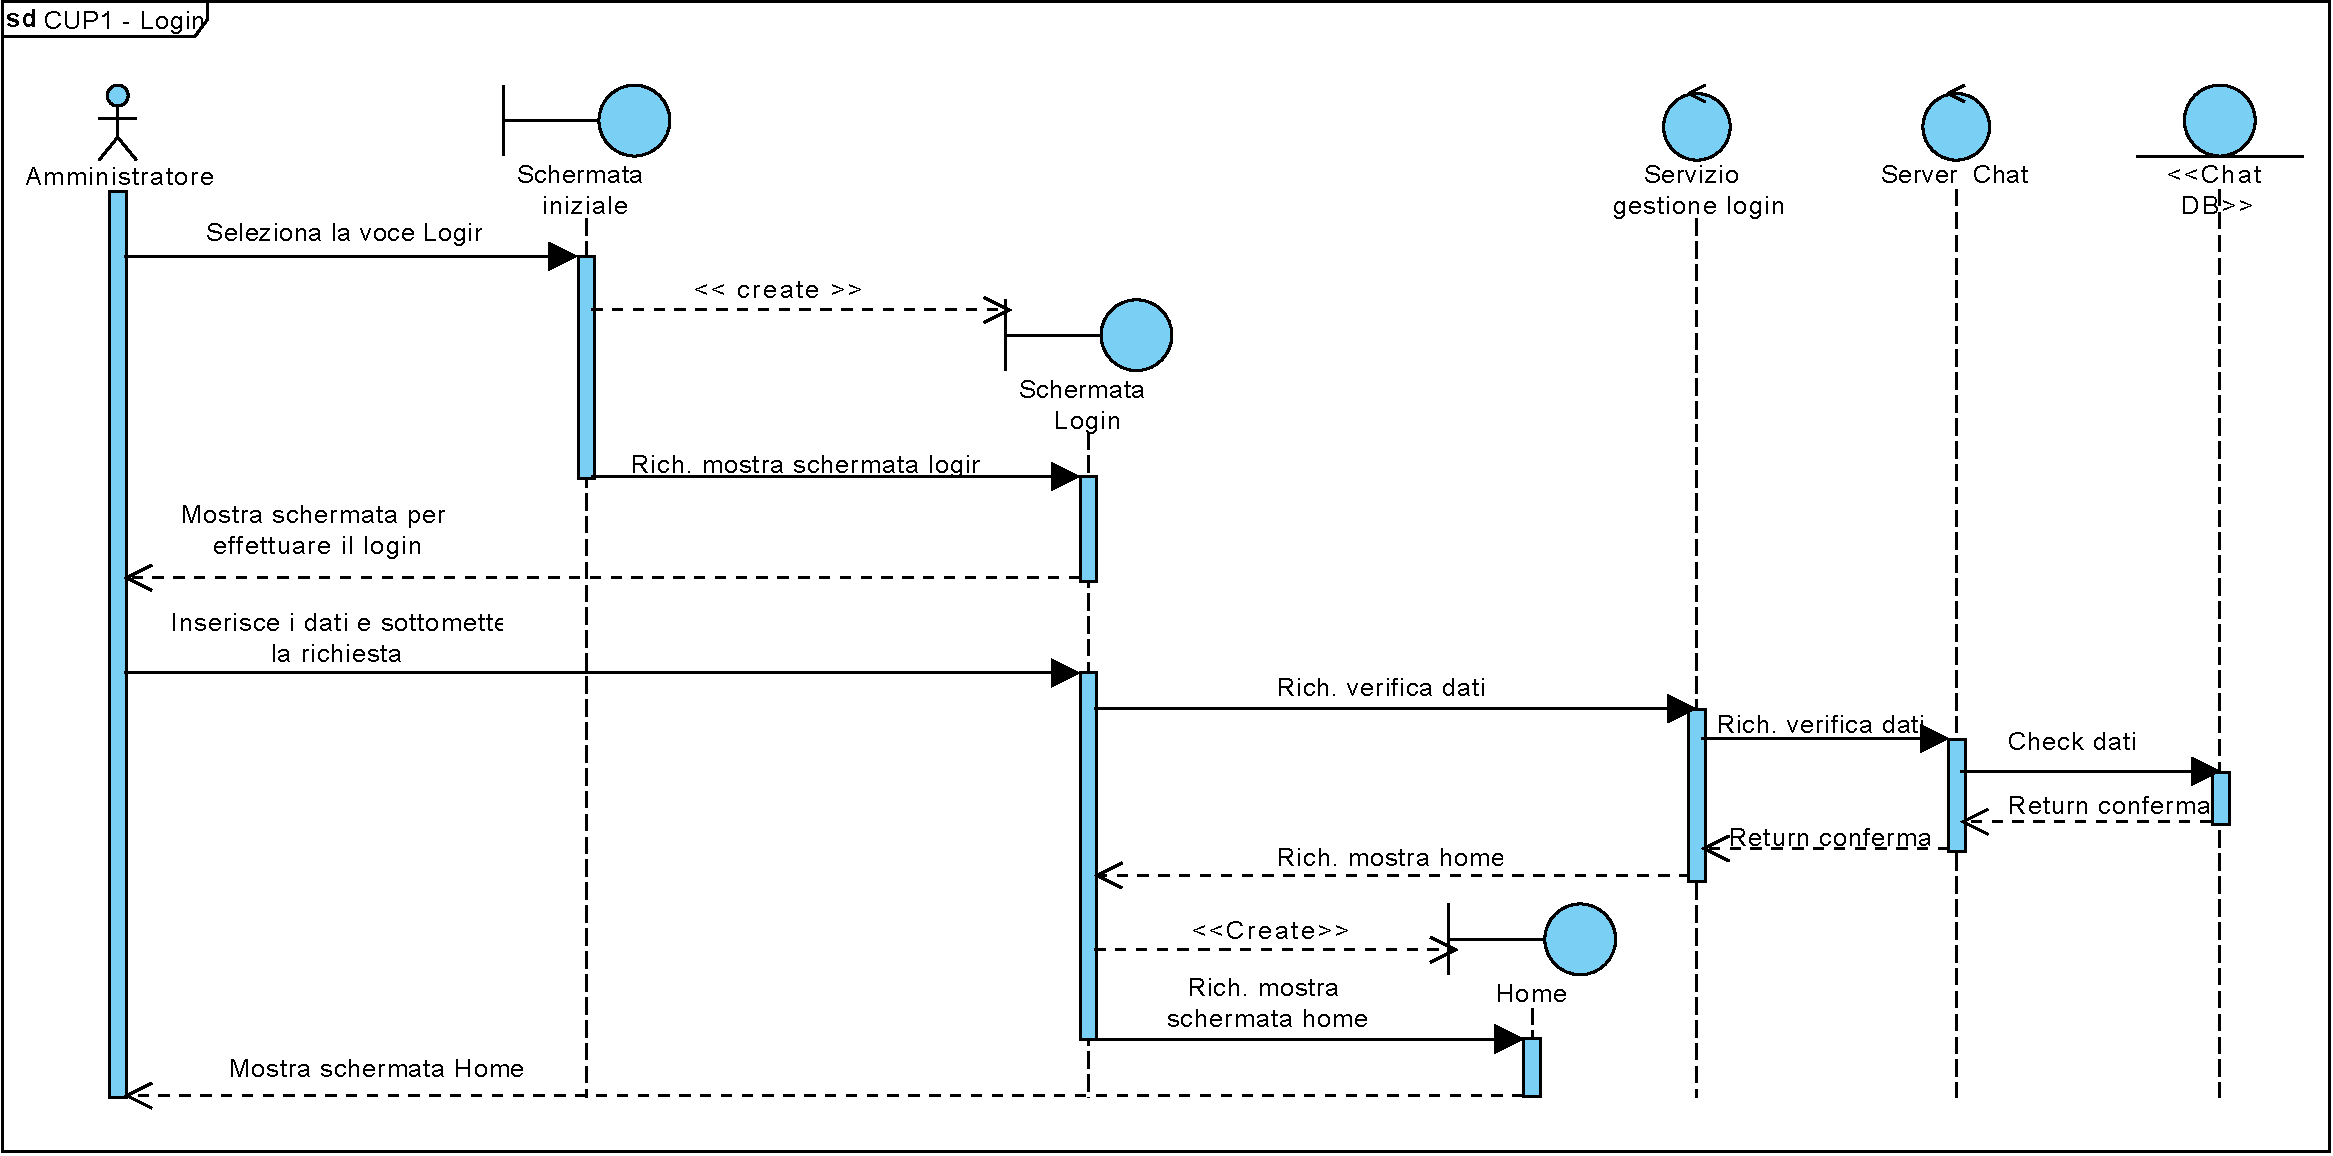
\includegraphics[height=3in,width=5in]{imgs/gruppo6/sequence/CUP1_Login.pdf}
	\caption{Login}
	\label{fig:prova}
\end{figure}

\begin{figure}
	\centering
	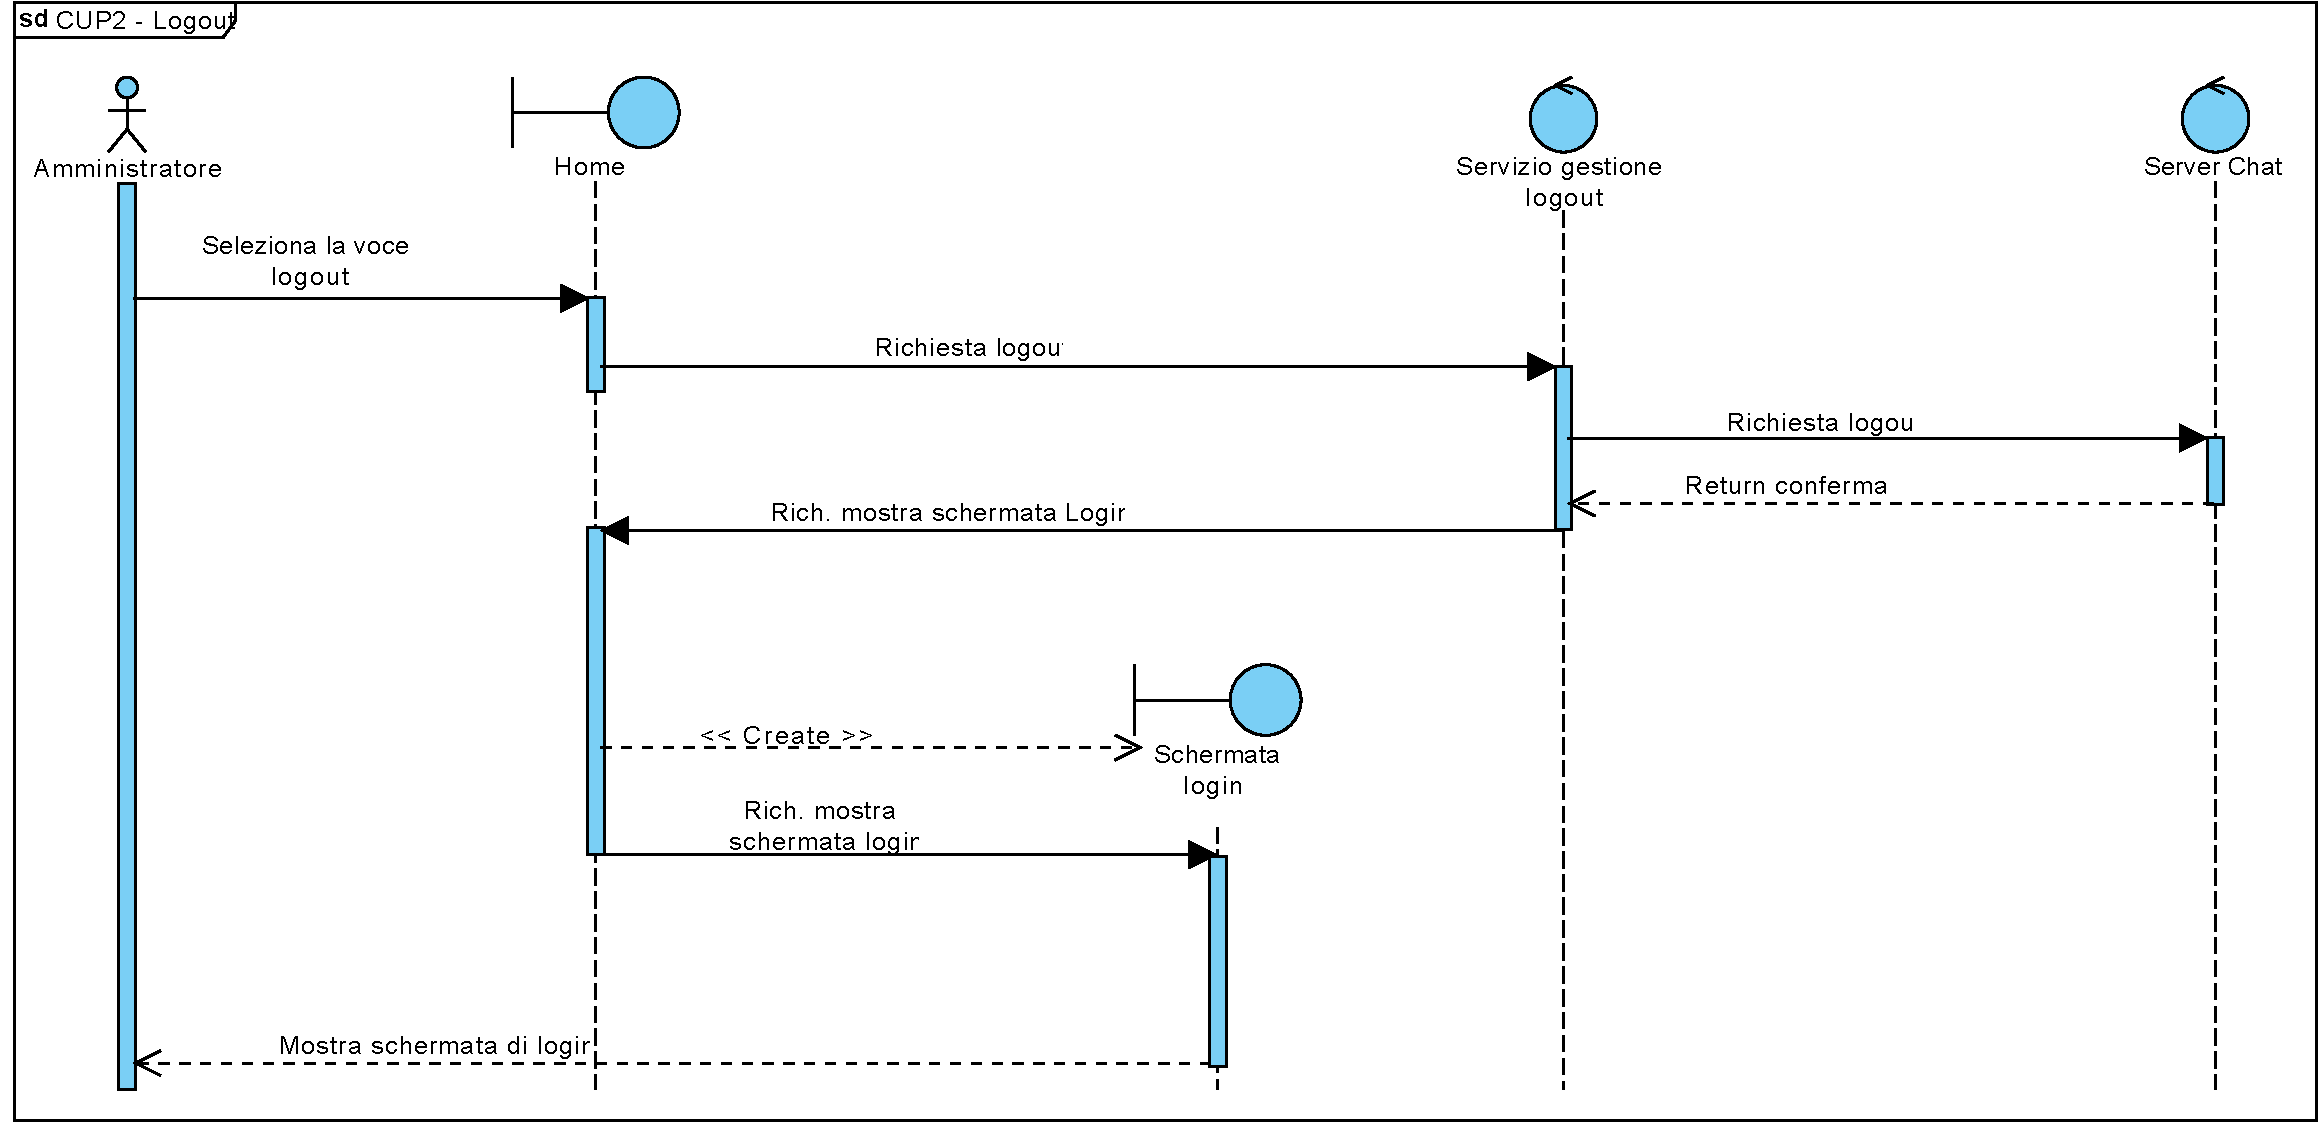
\includegraphics[height=3in,width=5in]{imgs/gruppo6/sequence/CUP2_logout.pdf}
	\caption{Logout}
	\label{fig:prova}
\end{figure}

\begin{figure}
	\centering
	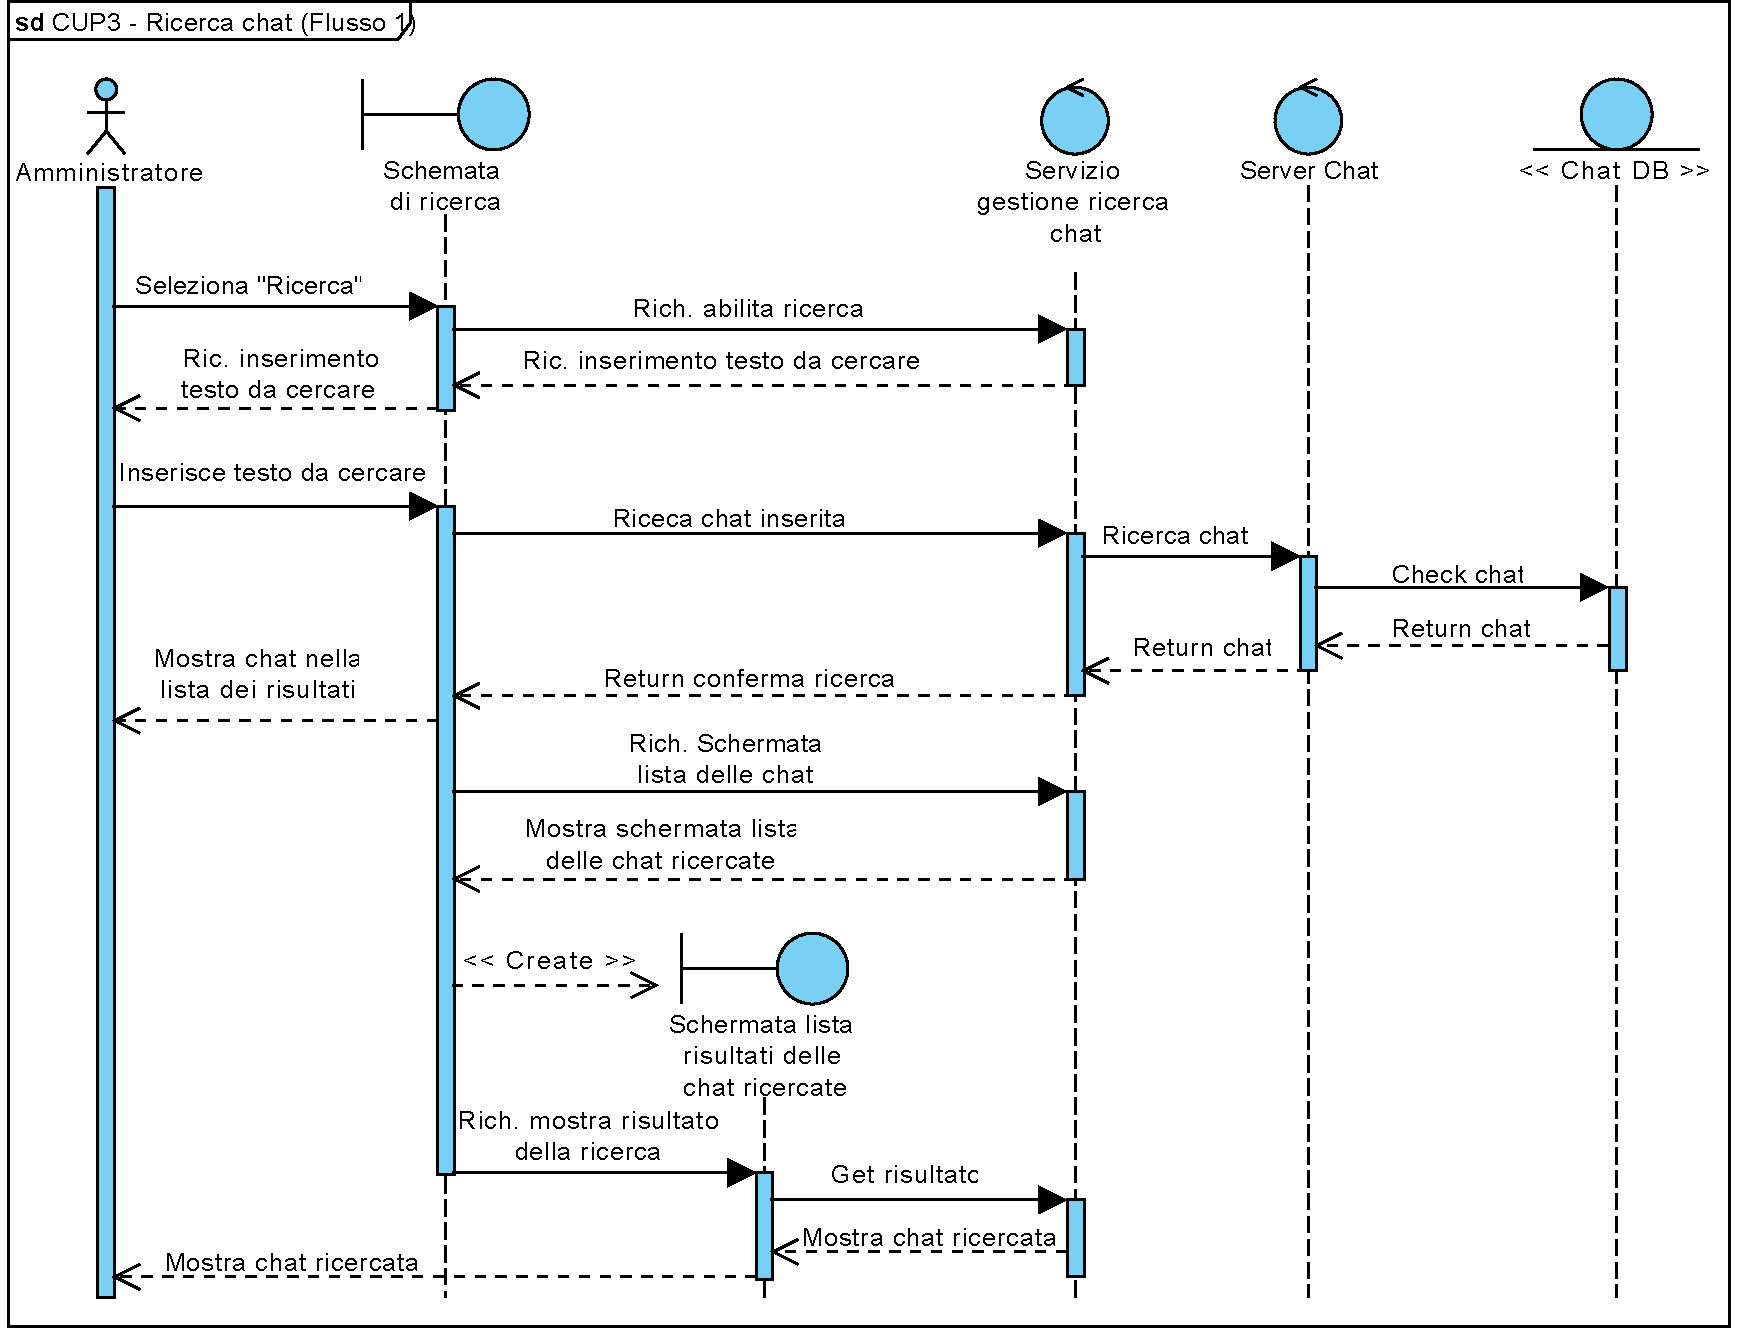
\includegraphics[height=3in,width=5in]{imgs/gruppo6/sequence/CUP3_ricerca_chat_flusso_1.pdf}
	\caption{Ricerca chat}
	\label{fig:prova}
\end{figure}

\begin{figure}
	\centering
	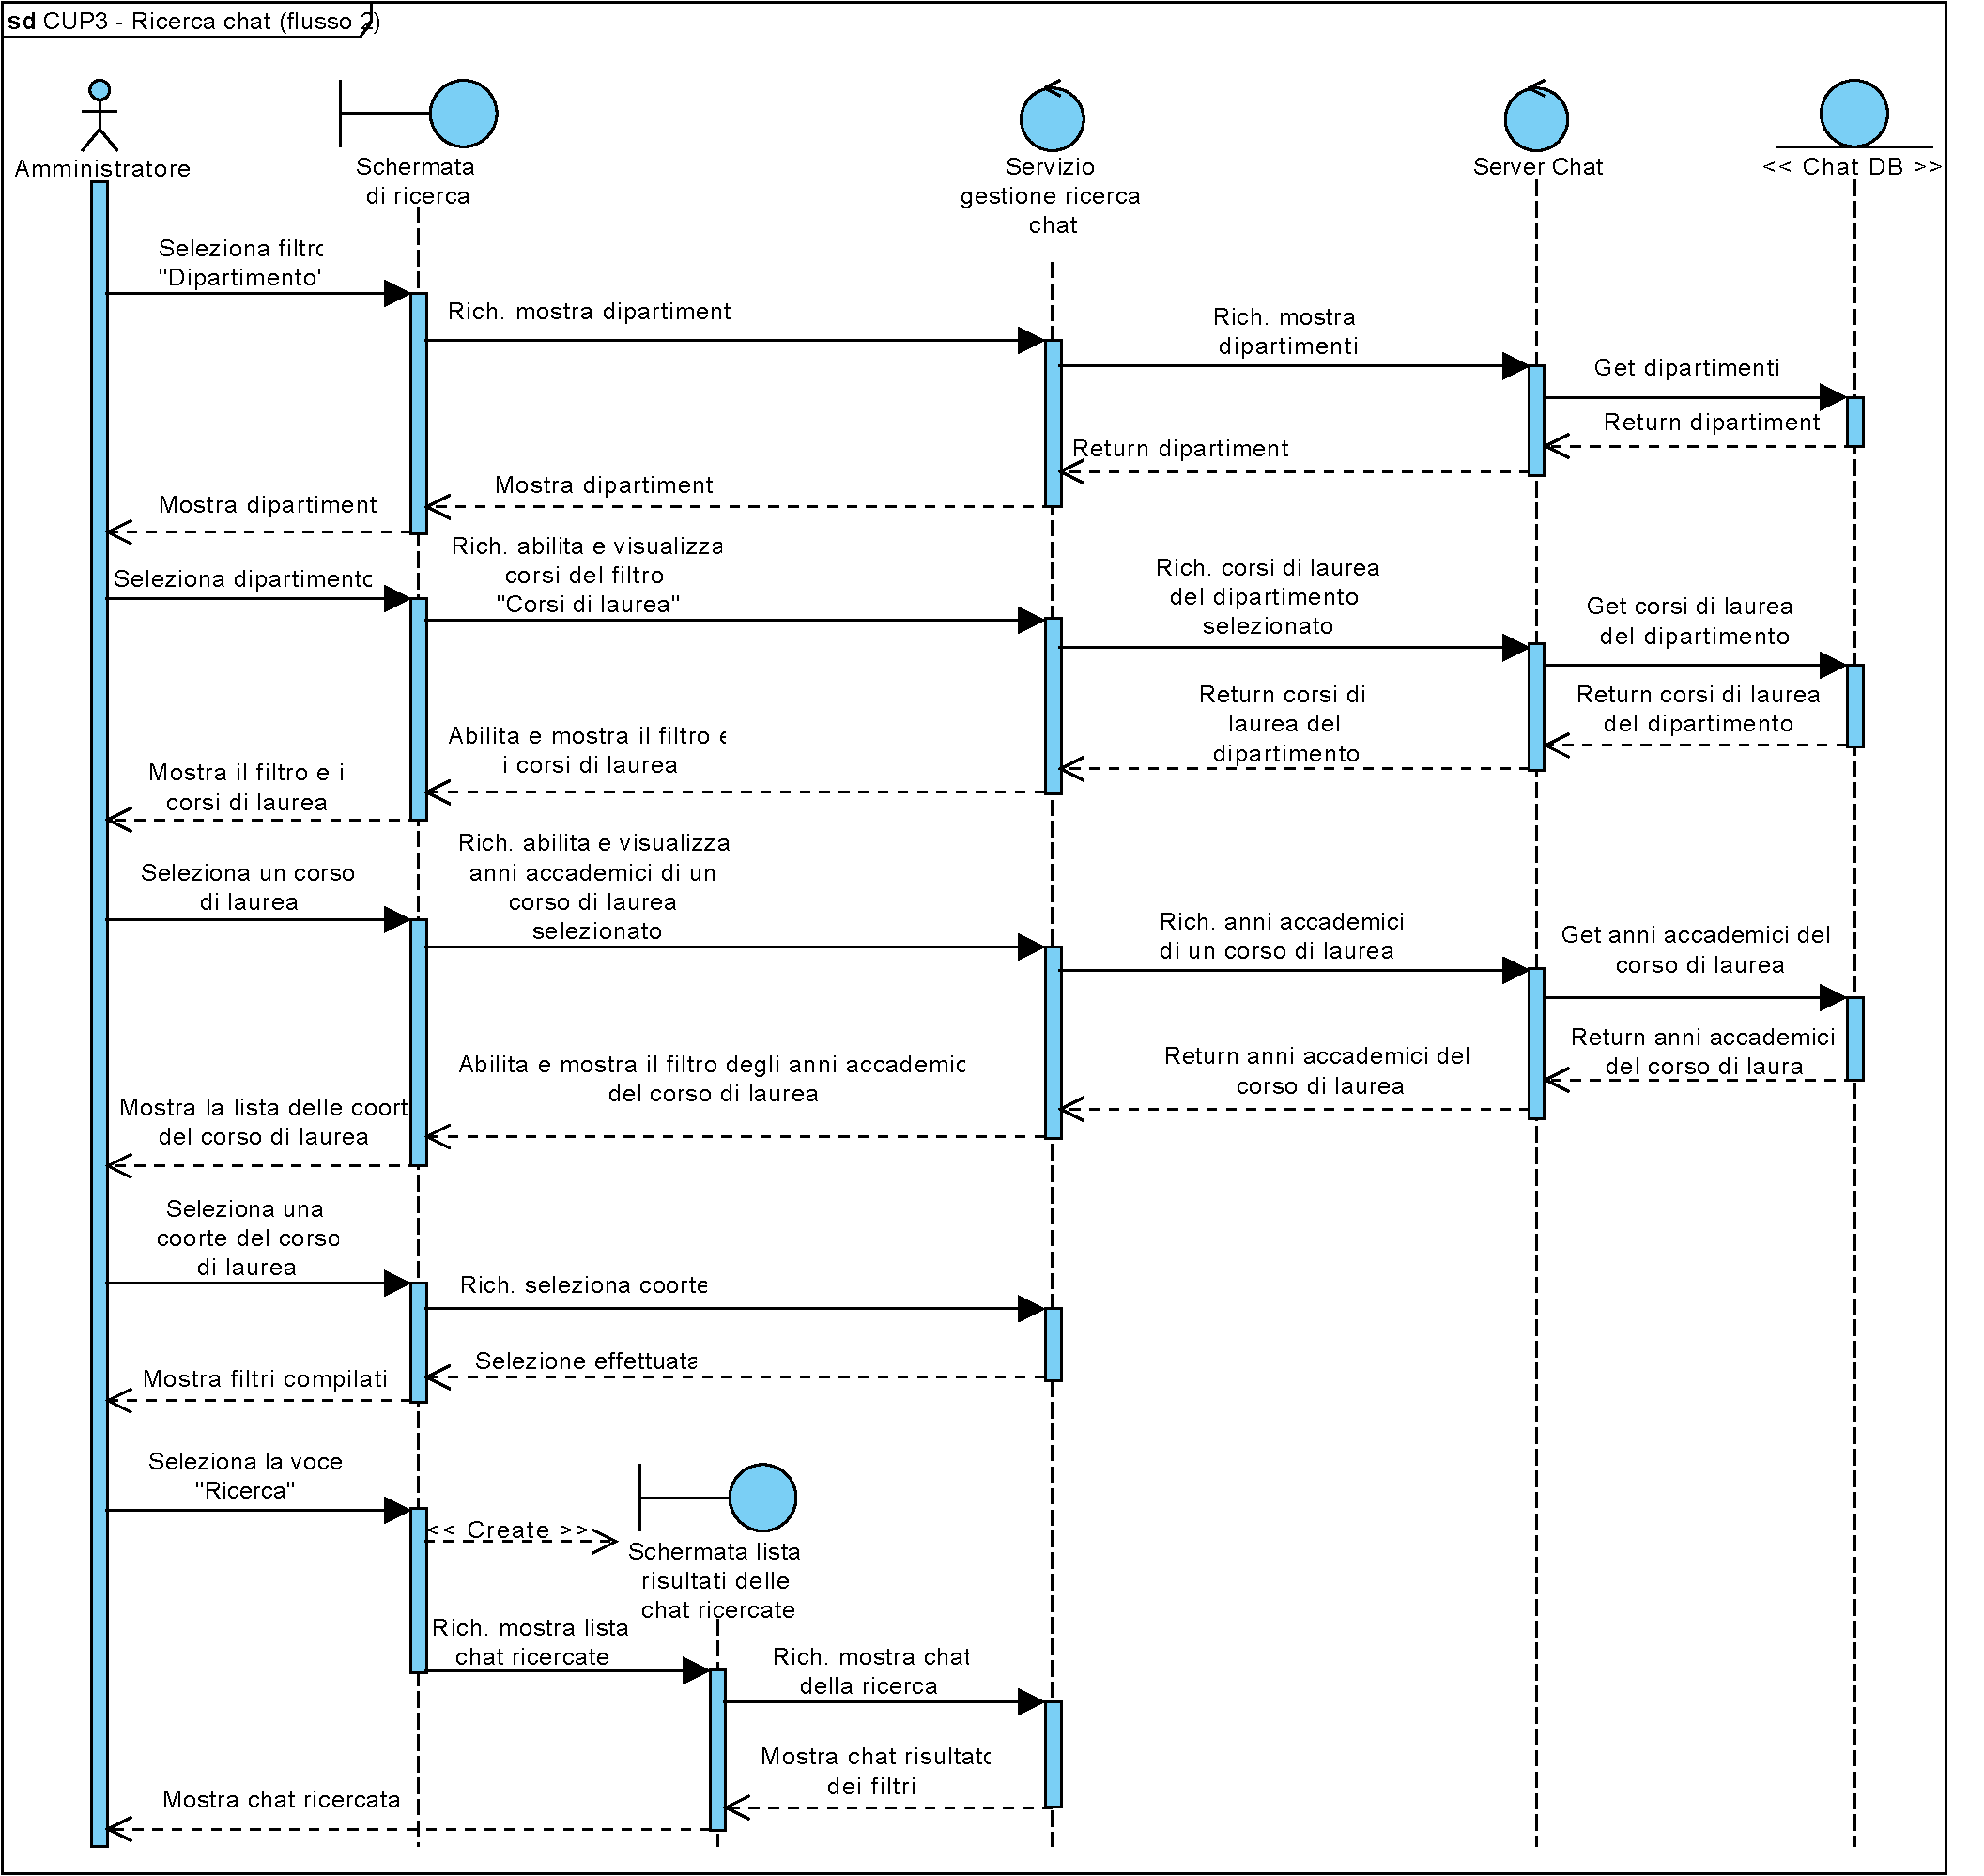
\includegraphics[height=3in,width=5in]{imgs/gruppo6/sequence/CUP3_ricerca_chat_flusso_2.pdf}
	\caption{Ricerca chat flusso alternativo}
	\label{fig:prova}
\end{figure}

\begin{figure}
	\centering
	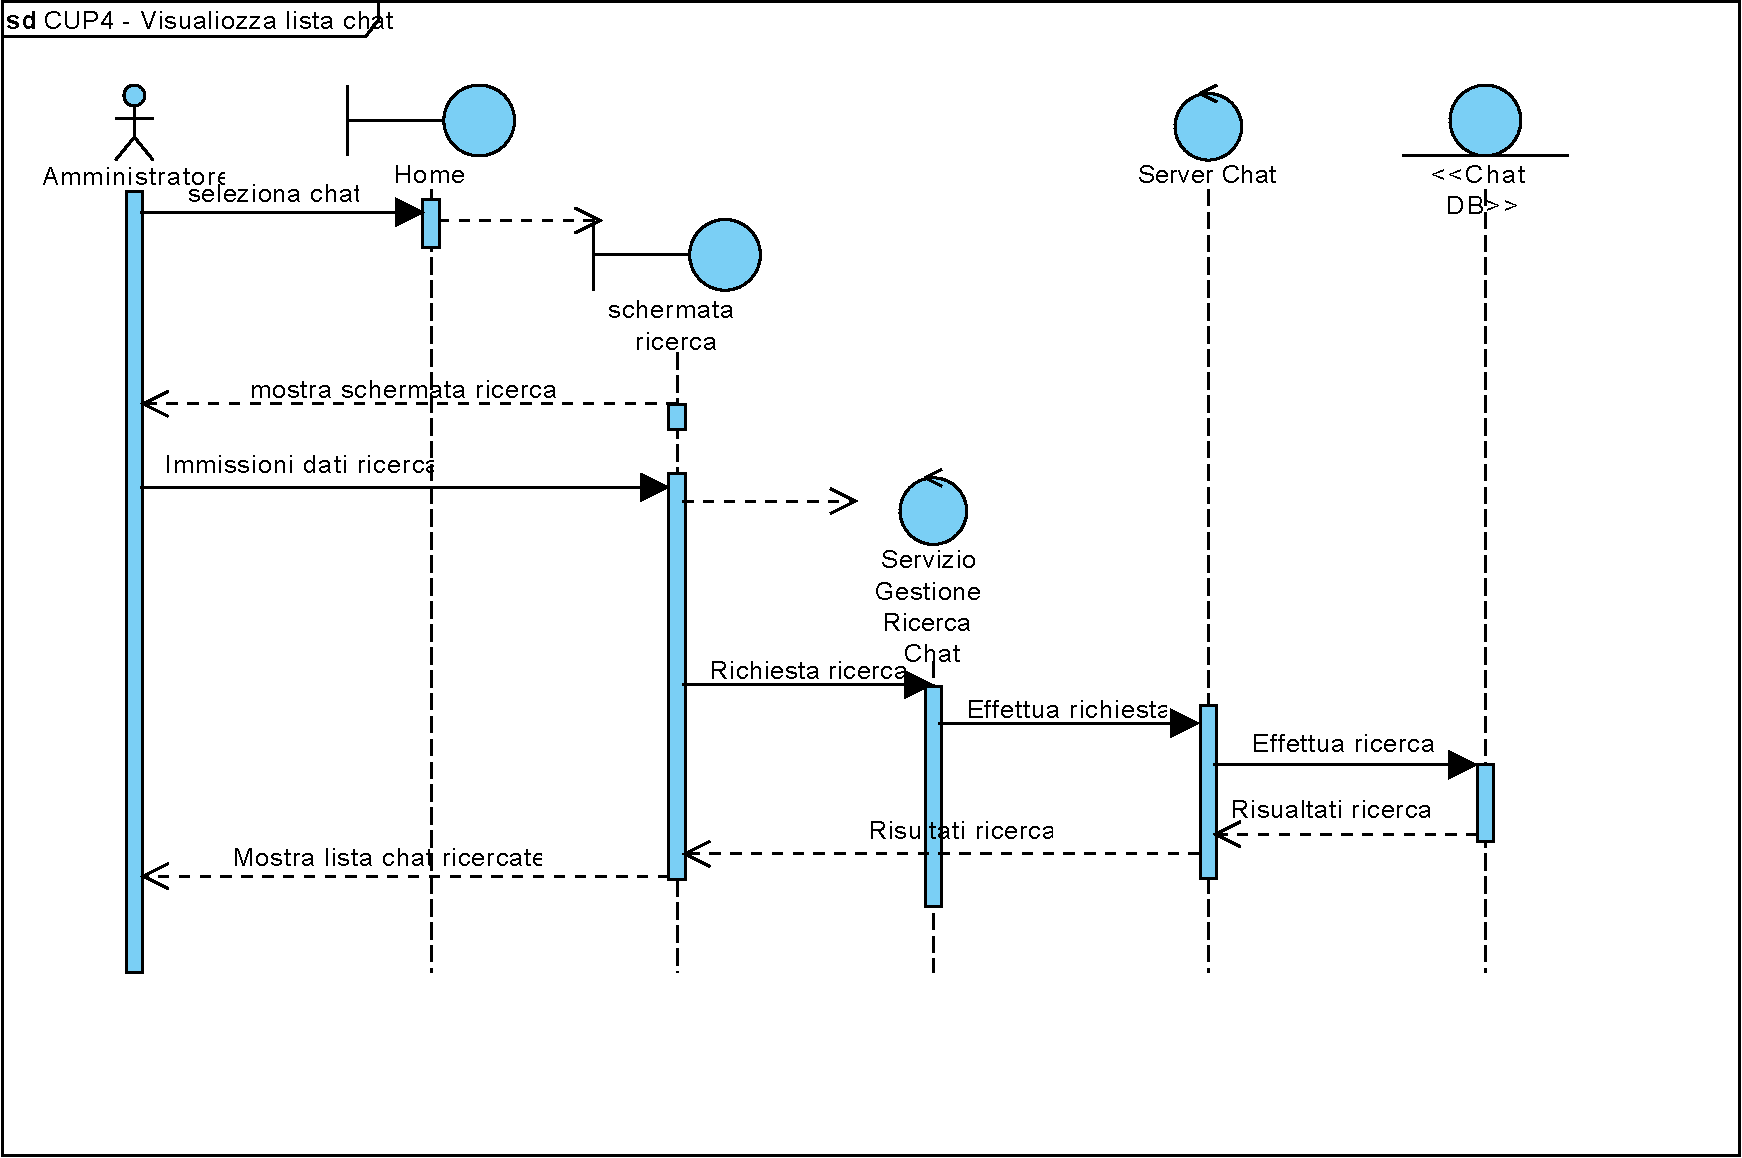
\includegraphics[height=3in,width=5in]{imgs/gruppo6/sequence/CUP4_visualizza_lista_chat.pdf}
	\caption{Visualizza lista chat}
	\label{fig:prova}
\end{figure}

\begin{figure}
	\centering
	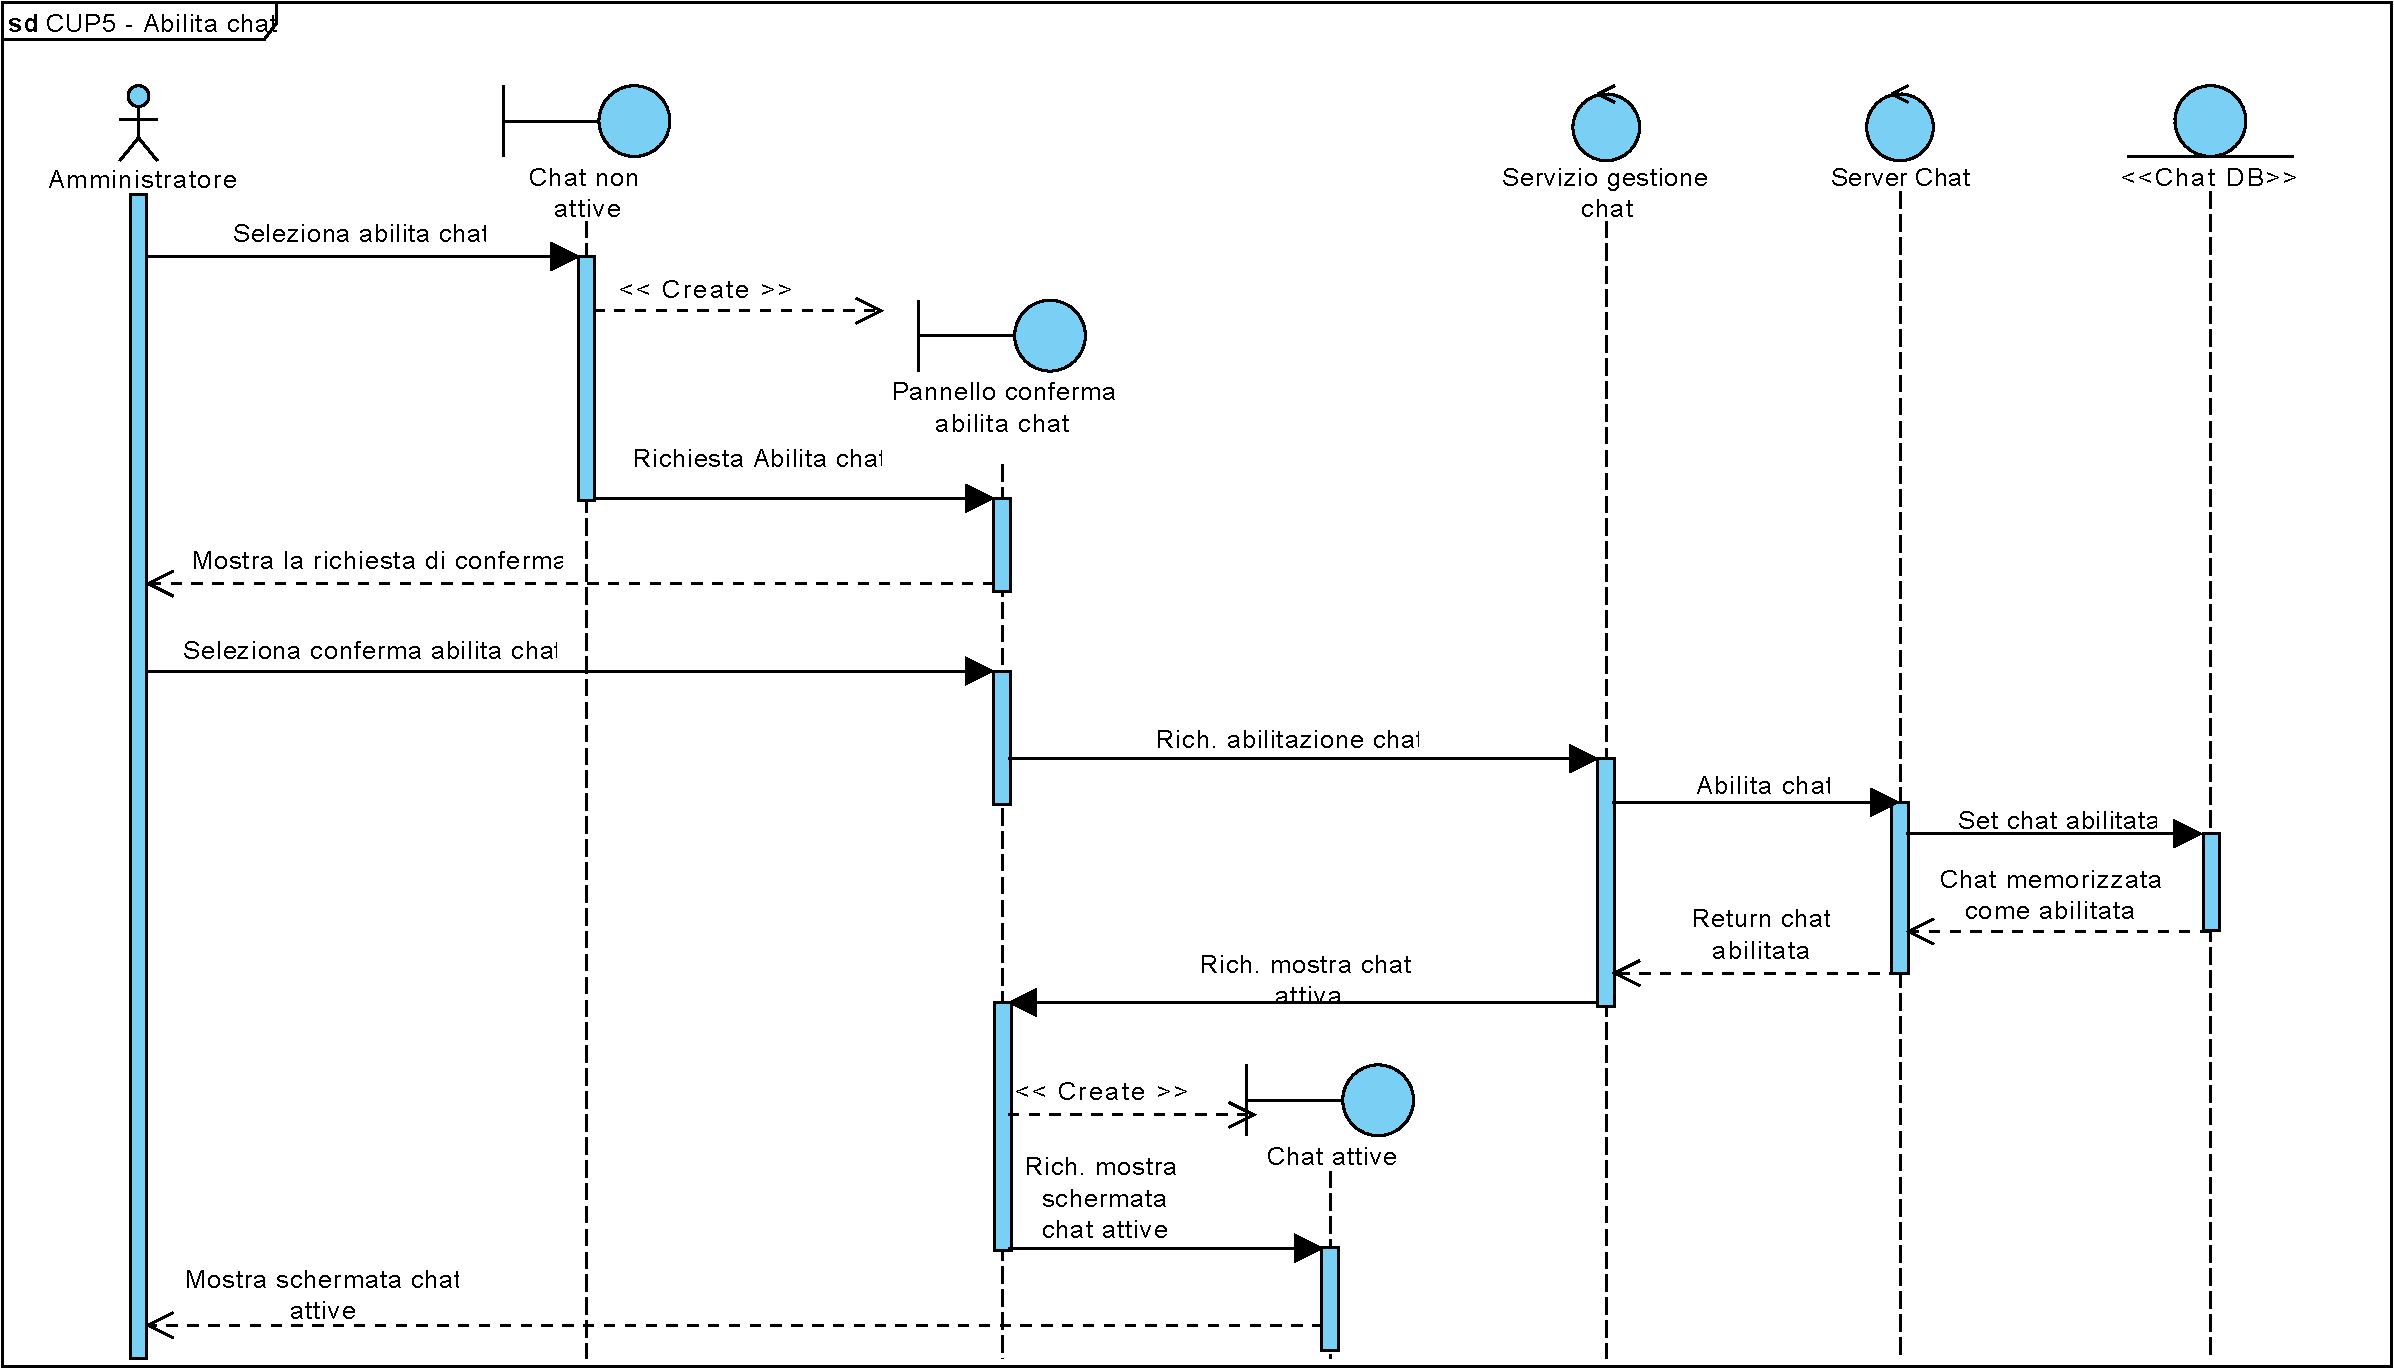
\includegraphics[height=3in,width=5in]{imgs/gruppo6/sequence/CUP5_abilita_chat.pdf}
	\caption{Abilita chat}
	\label{fig:prova}
\end{figure}

\begin{figure}
	\centering
	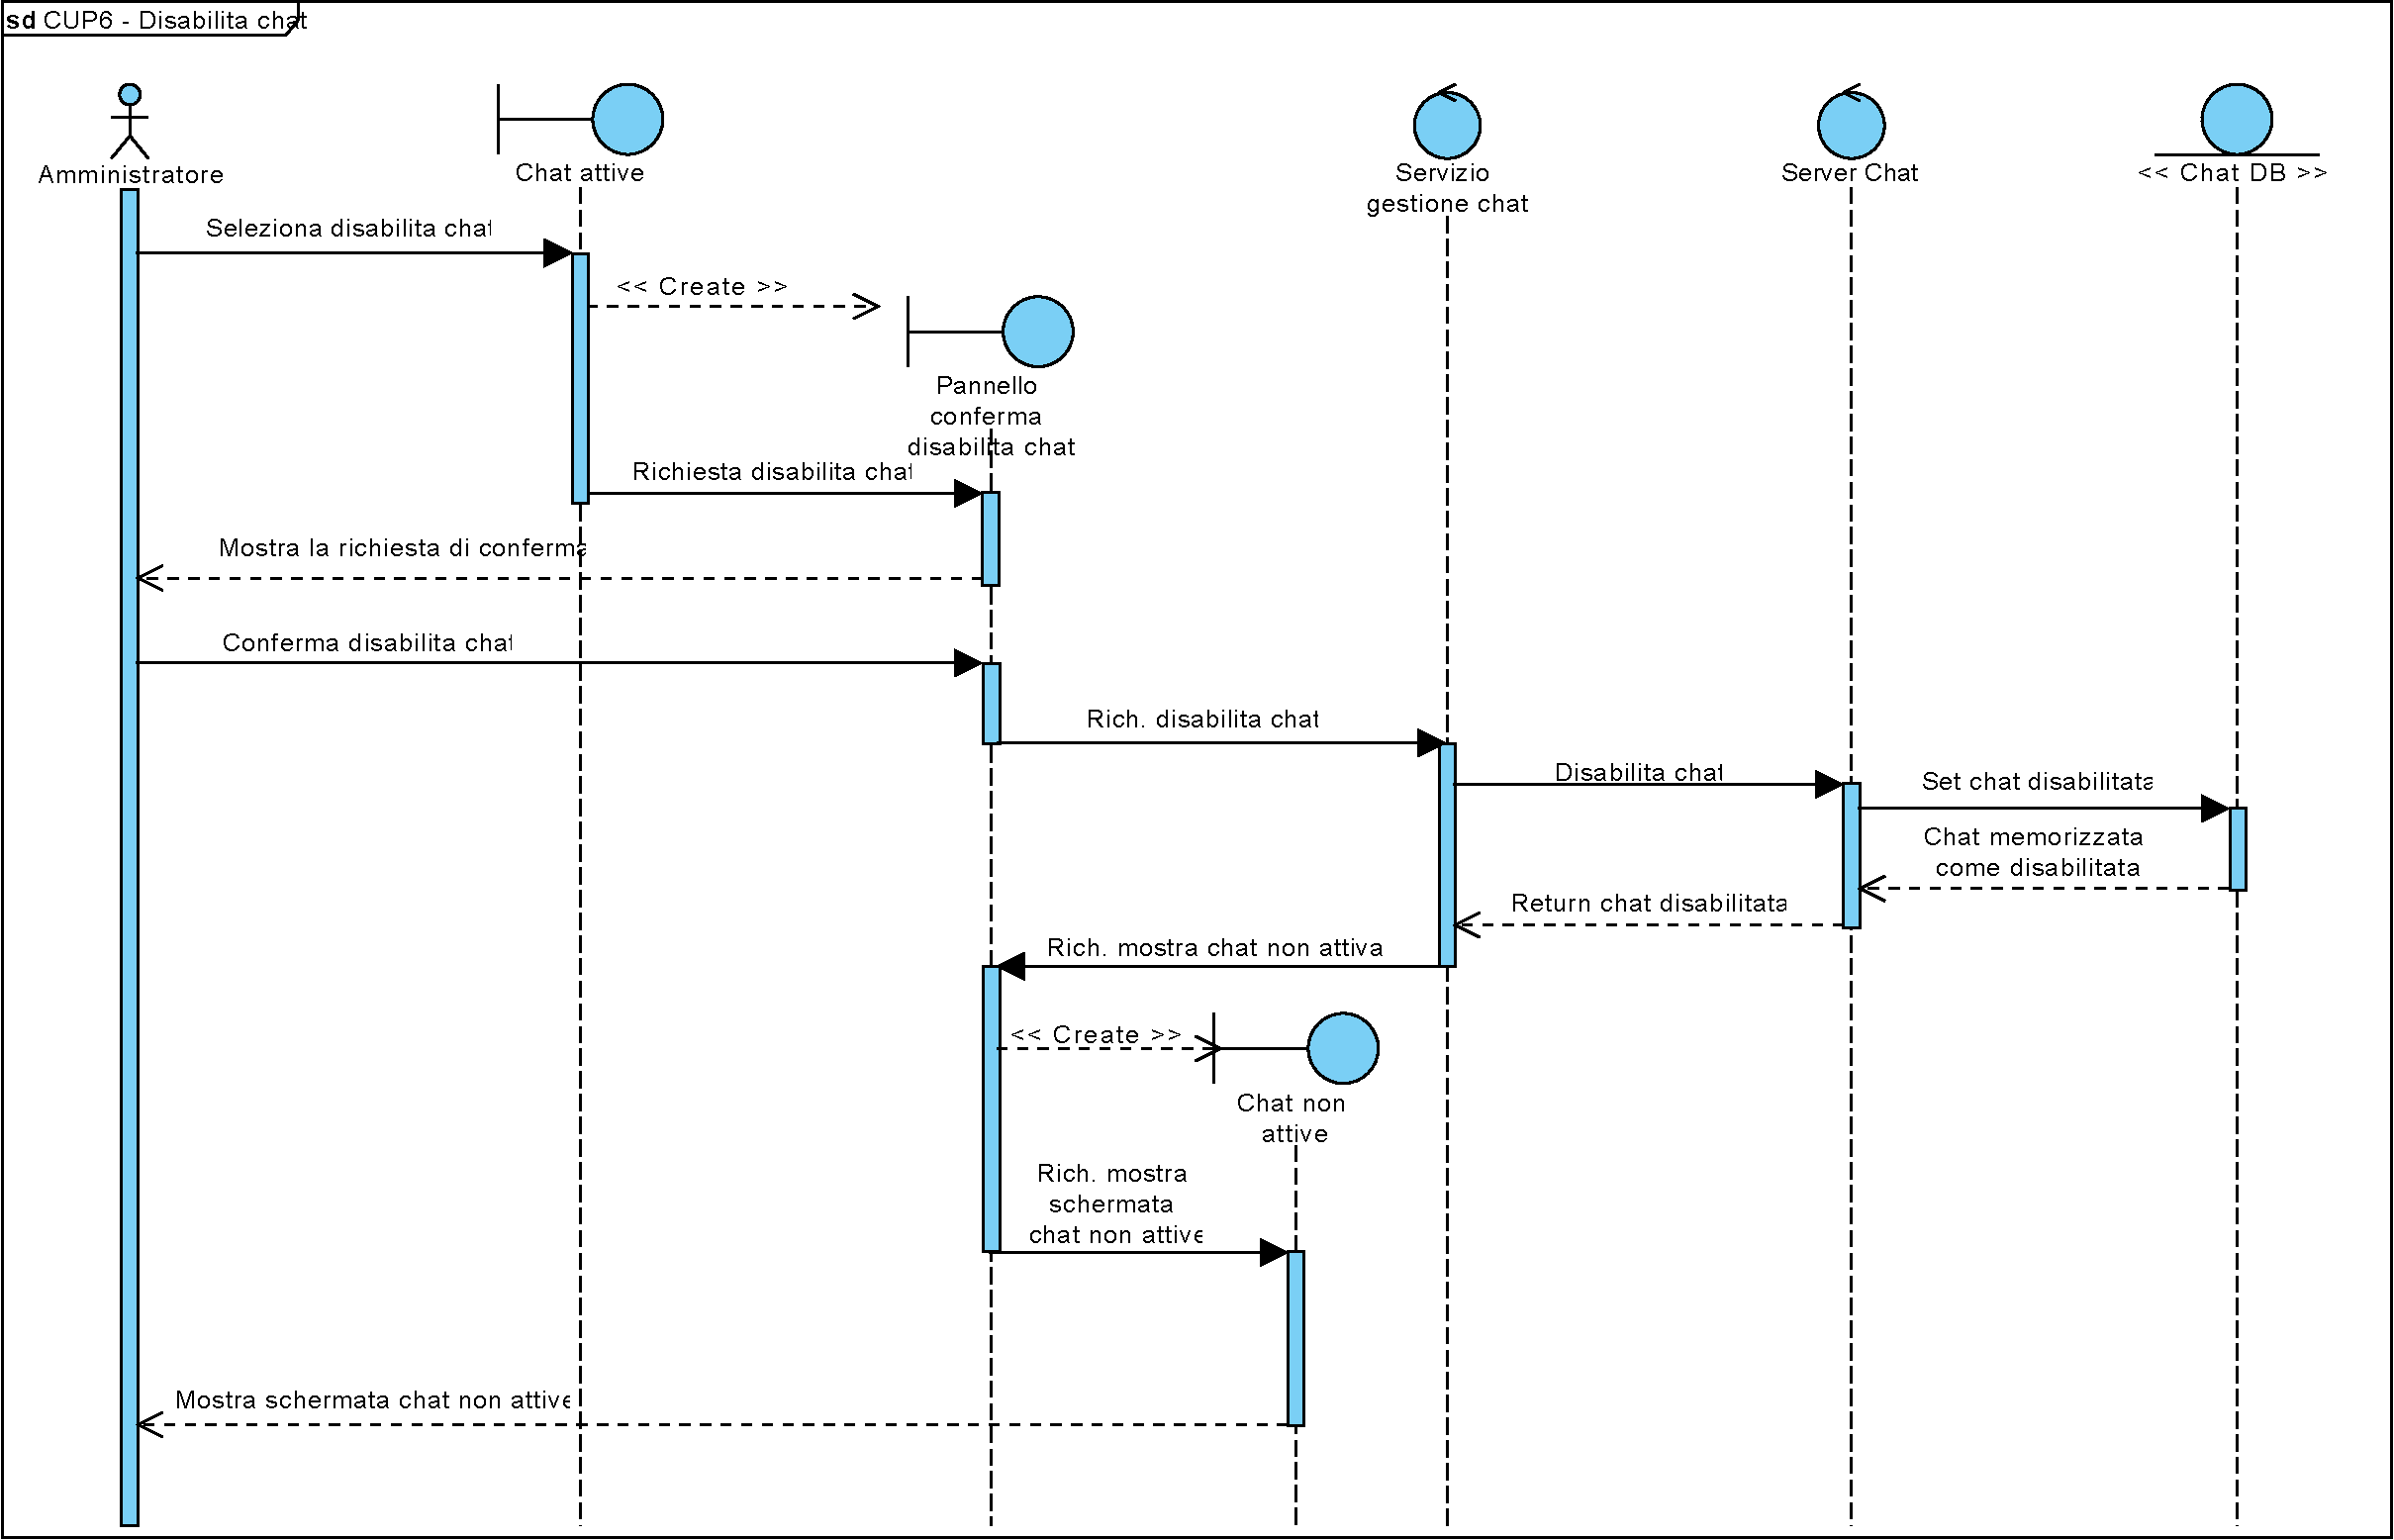
\includegraphics[height=3in,width=5in]{imgs/gruppo6/sequence/CUP6_disabilita_chat.pdf}
	\caption{Disabilita chat}
	\label{fig:prova}
\end{figure}

\begin{figure}
	\centering
	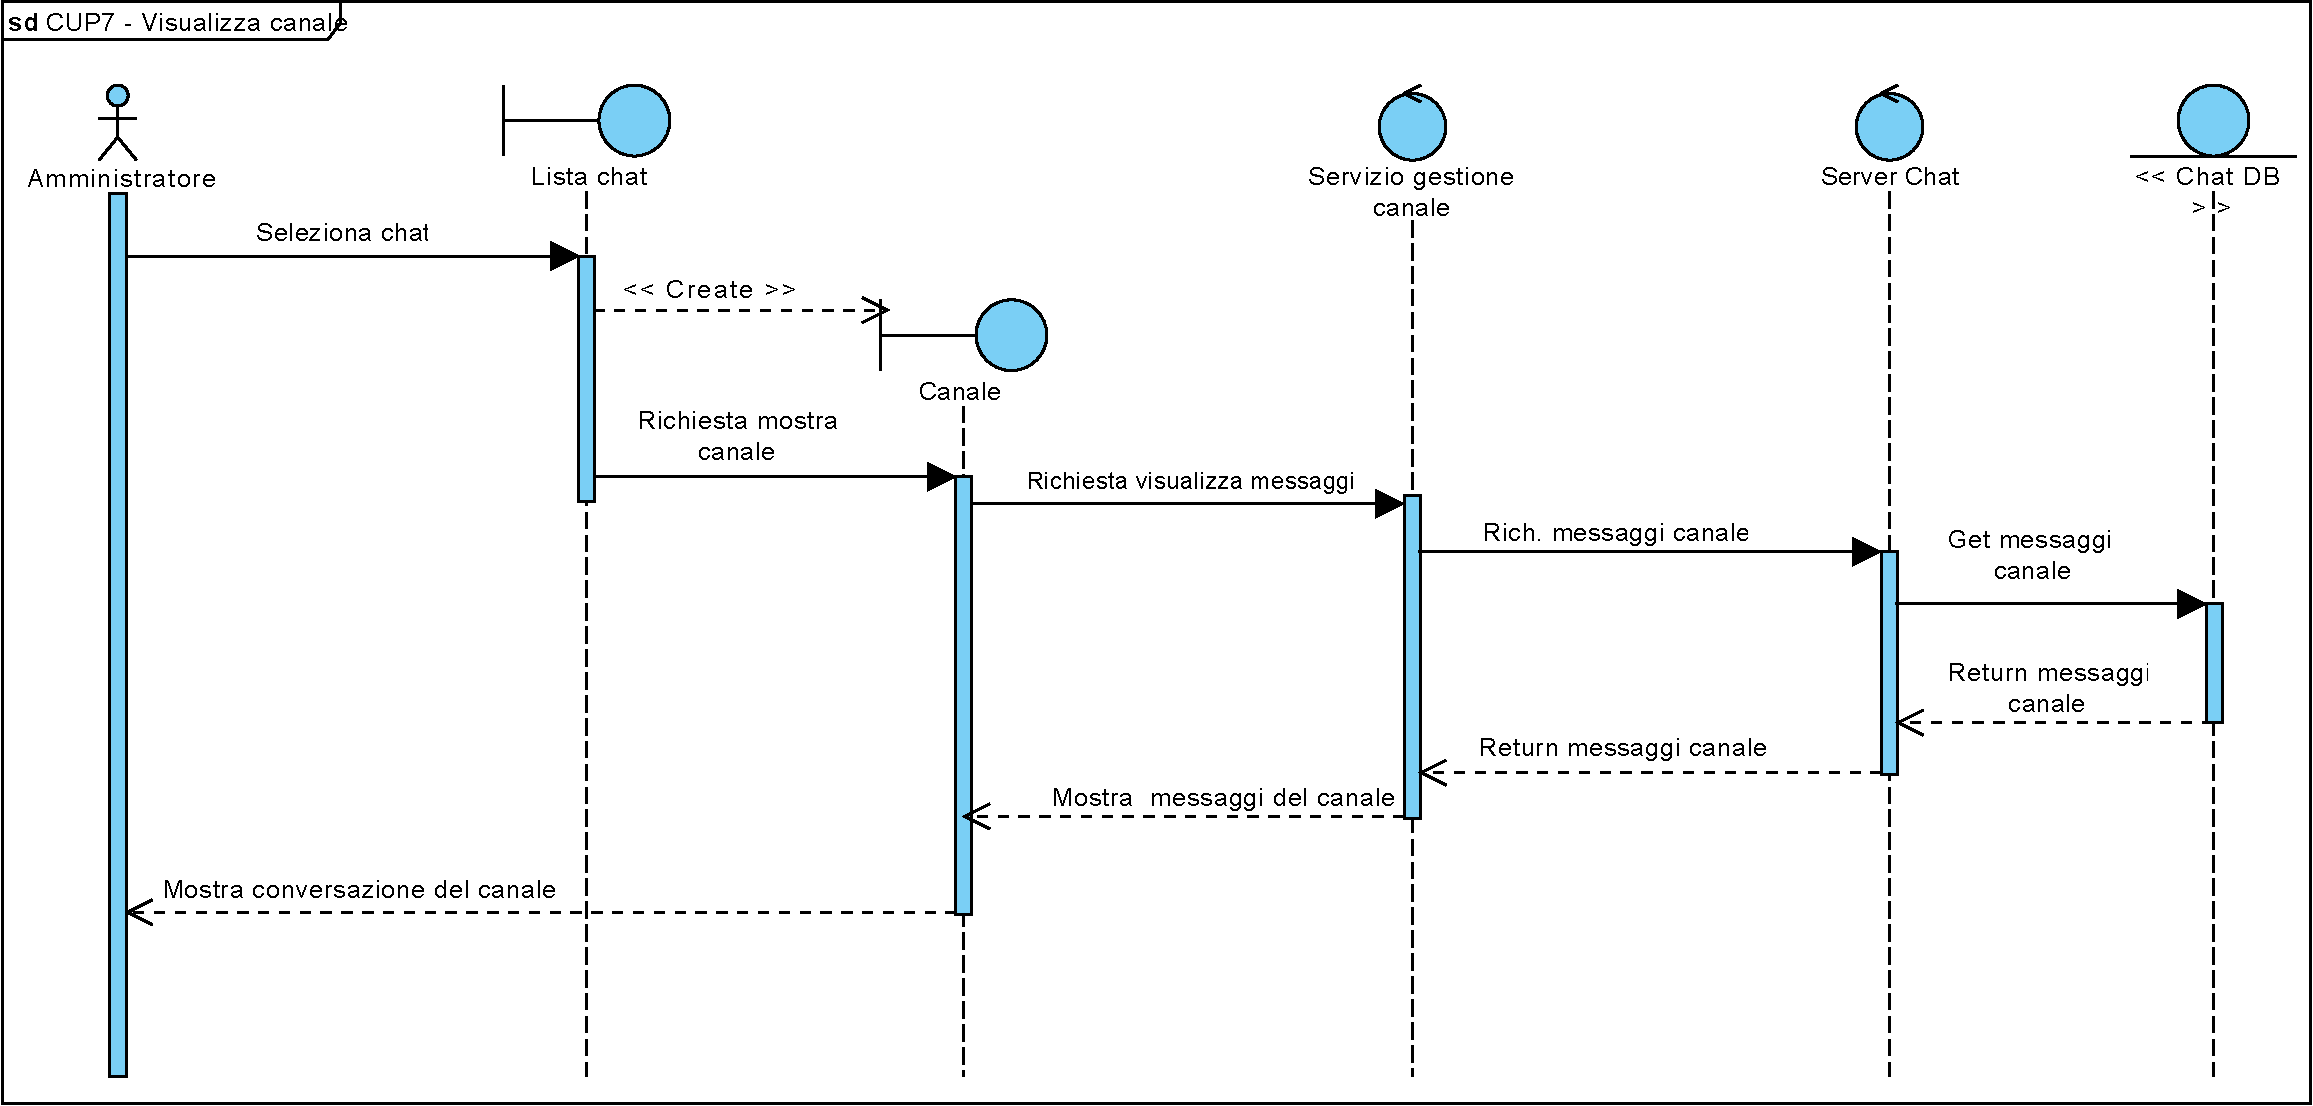
\includegraphics[height=3in,width=5in]{imgs/gruppo6/sequence/CUP7_visualizza_canale.pdf}
	\caption{Visualizza canale}
	\label{fig:prova}
\end{figure}

\begin{figure}
	\centering
	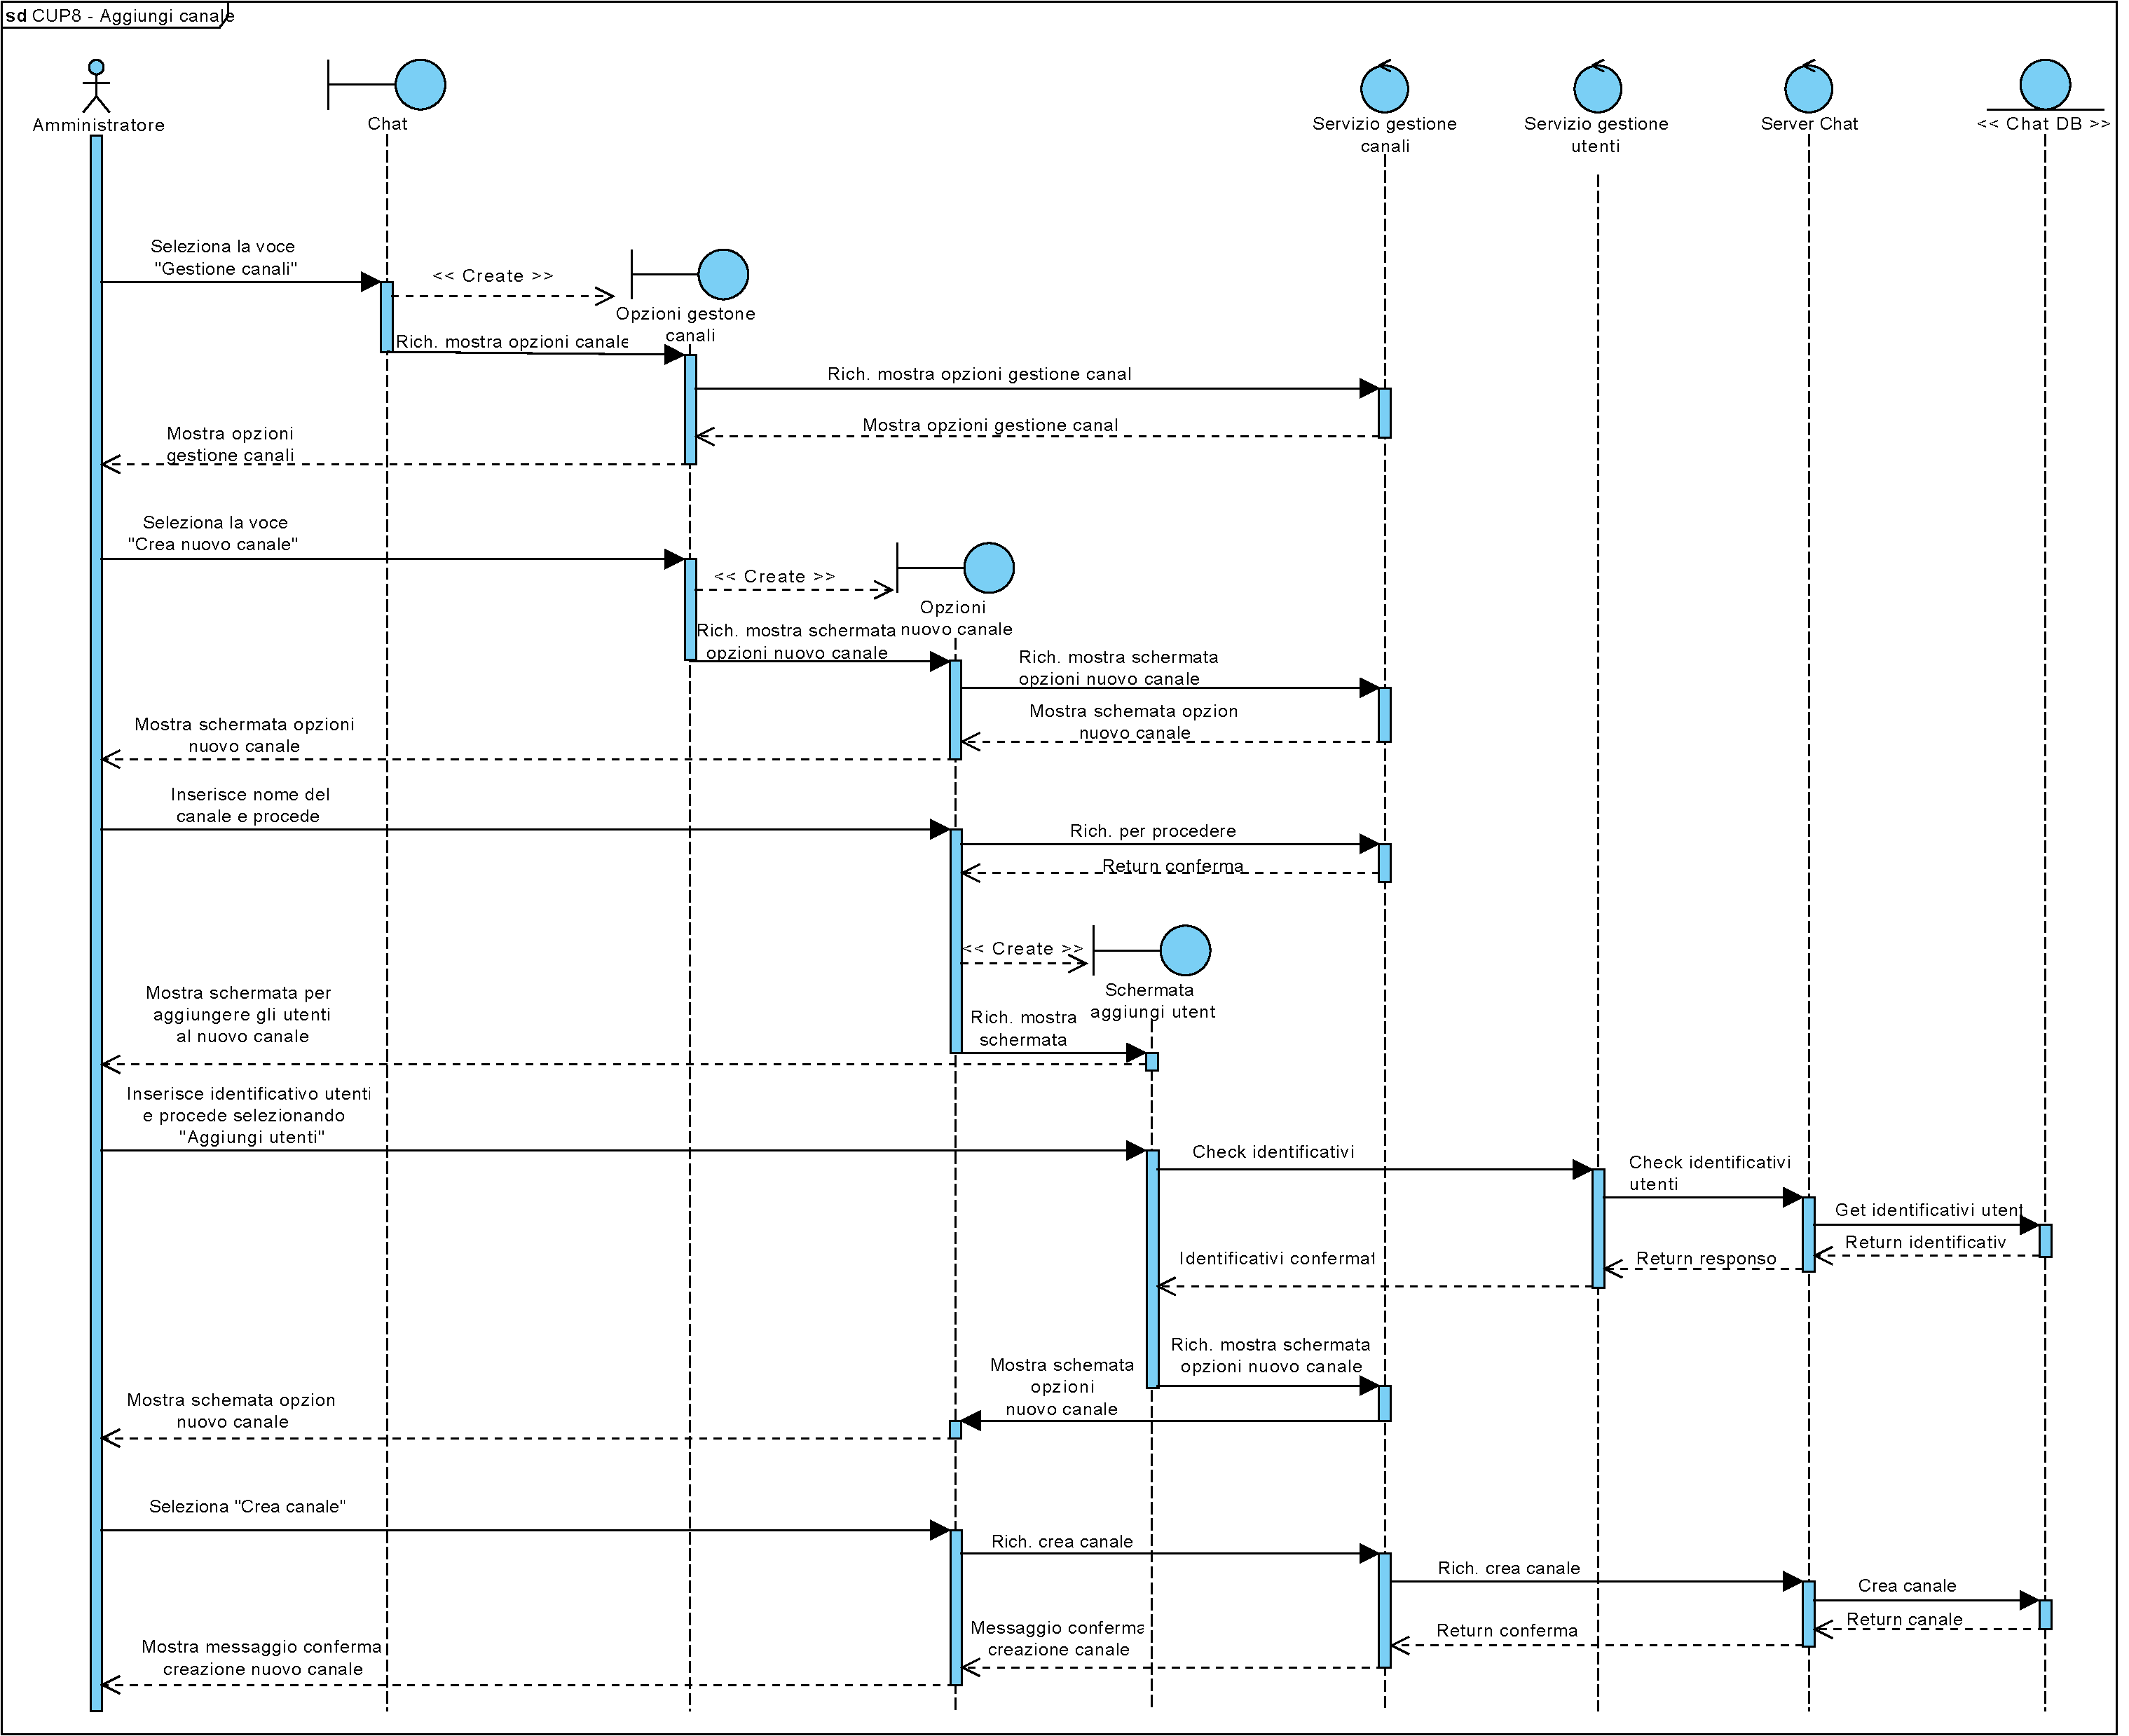
\includegraphics[height=3in,width=5in]{imgs/gruppo6/sequence/CUP8_aggiungi_canale.pdf}
	\caption{Aggiungi canale}
	\label{fig:prova}
\end{figure}

\begin{figure}
	\centering
	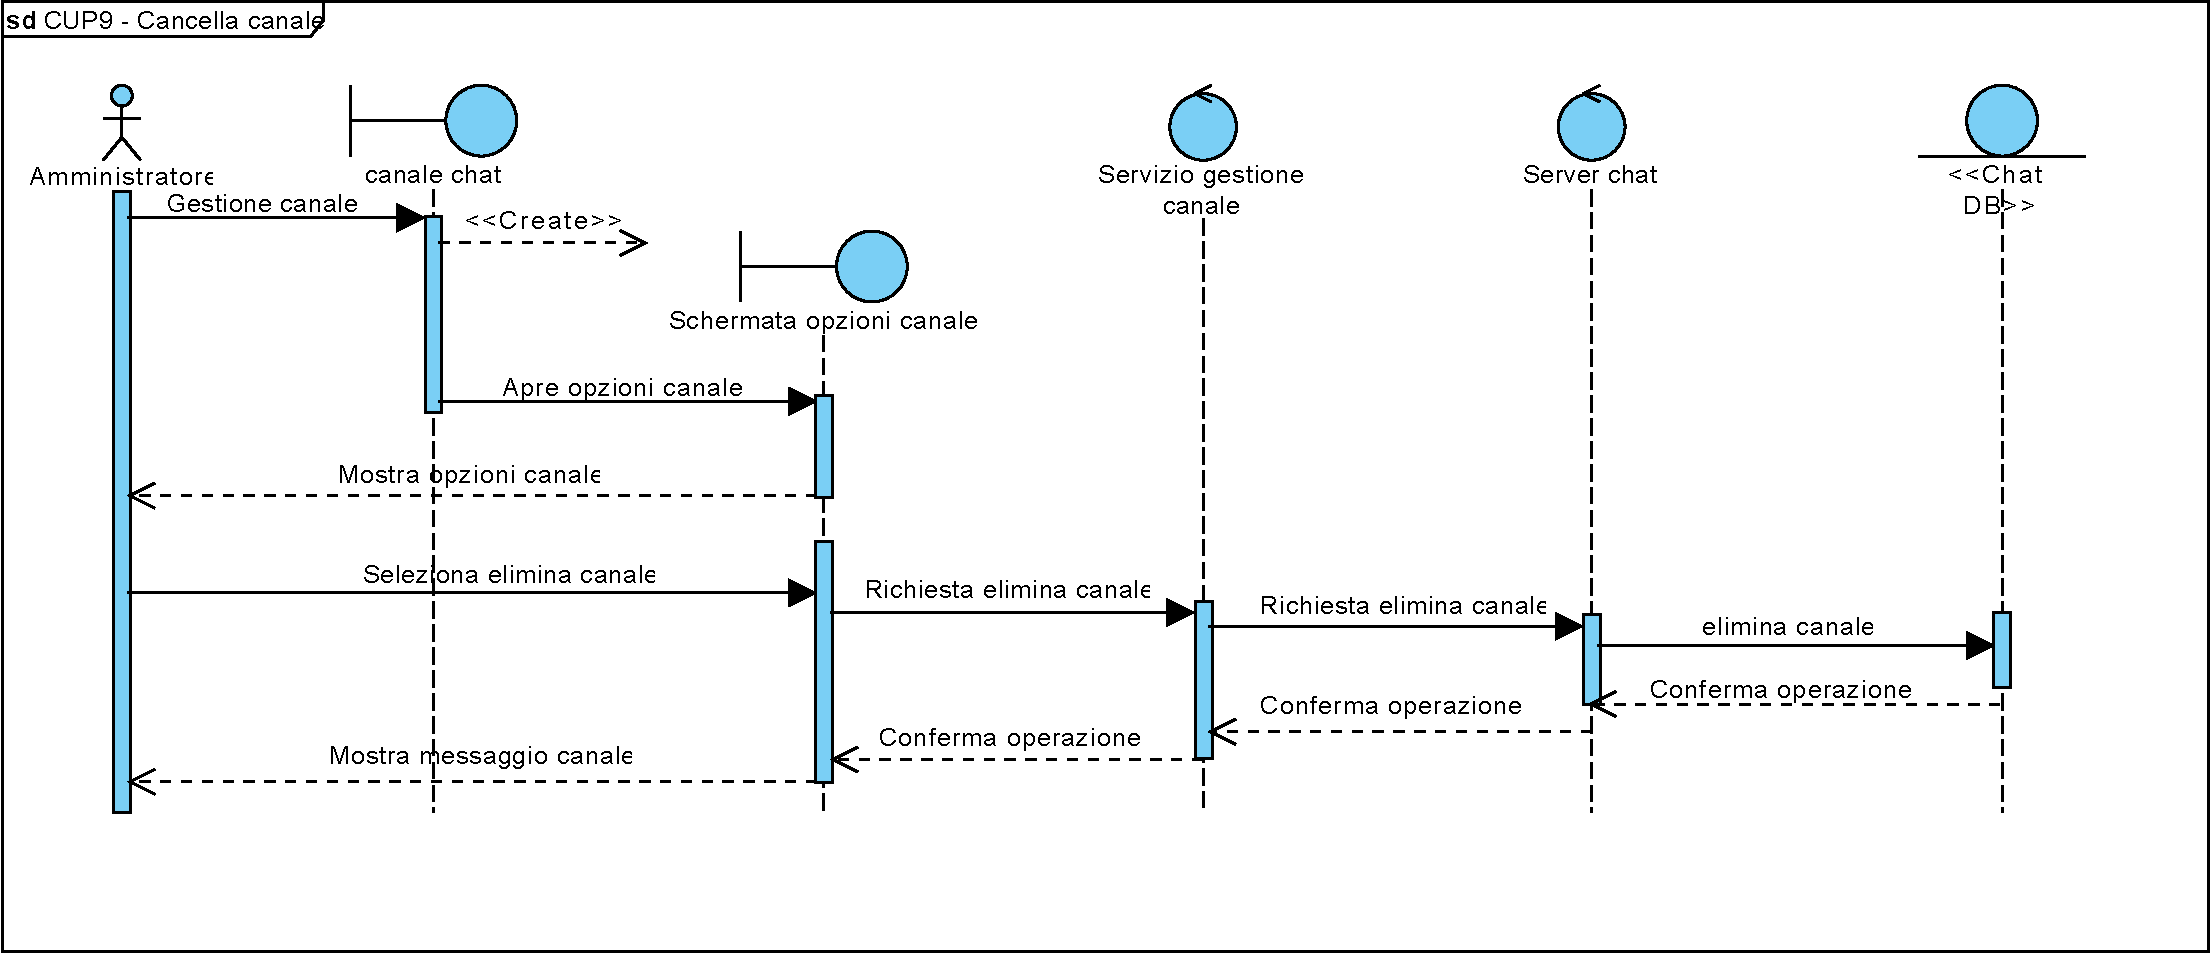
\includegraphics[height=3in,width=5in]{imgs/gruppo6/sequence/CUP9_cancella_canale.pdf}
	\caption{Cancella canale}
	\label{fig:prova}
\end{figure}

\begin{figure}
	\centering
	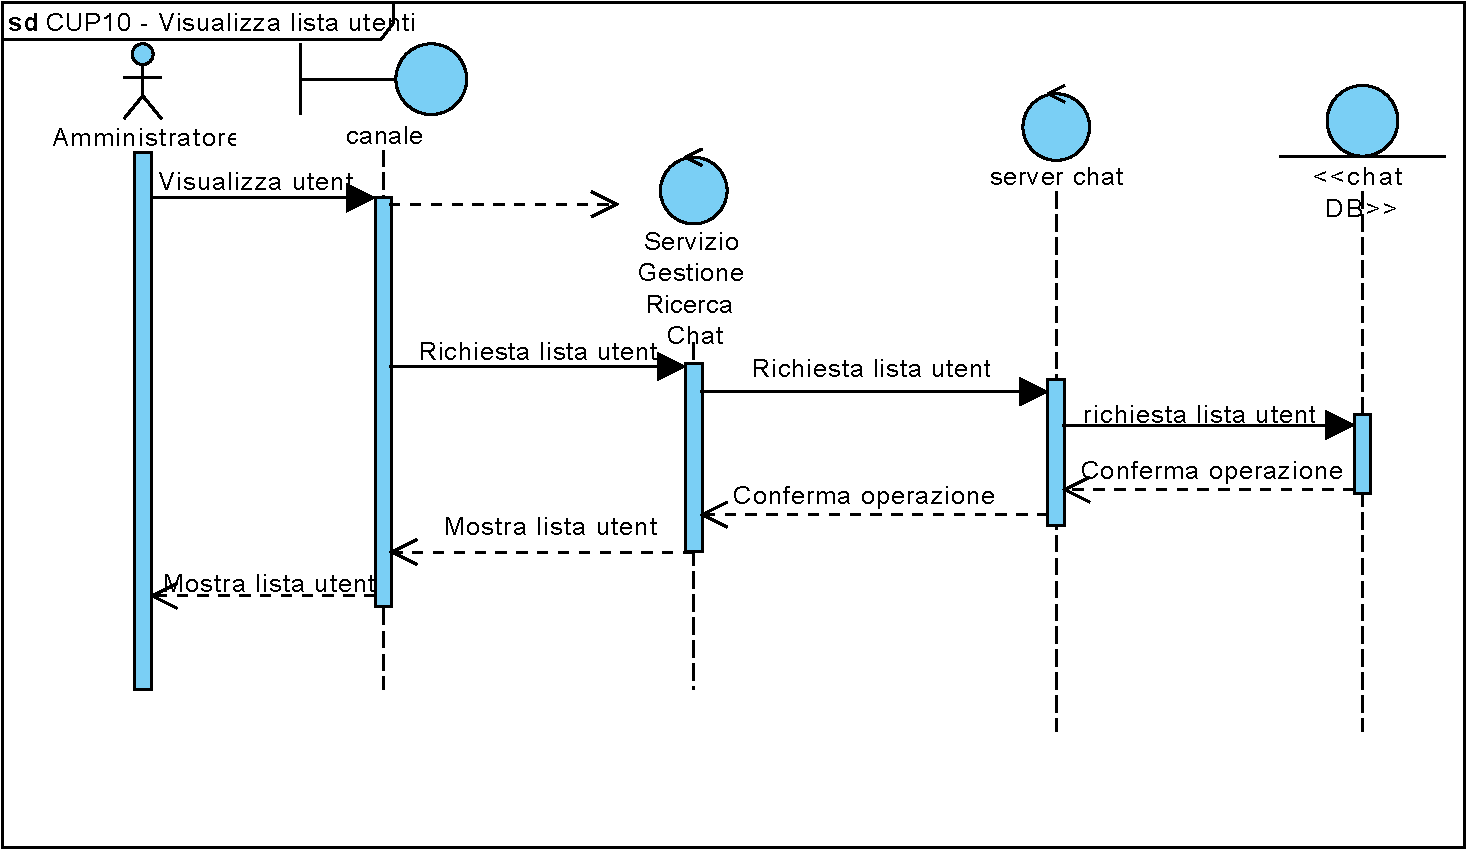
\includegraphics[height=3in,width=5in]{imgs/gruppo6/sequence/CUP10_visualizza_lista_utenti.pdf}
	\caption{Visualizza lista utenti}
	\label{fig:prova}
\end{figure}

\begin{figure}
	\centering
	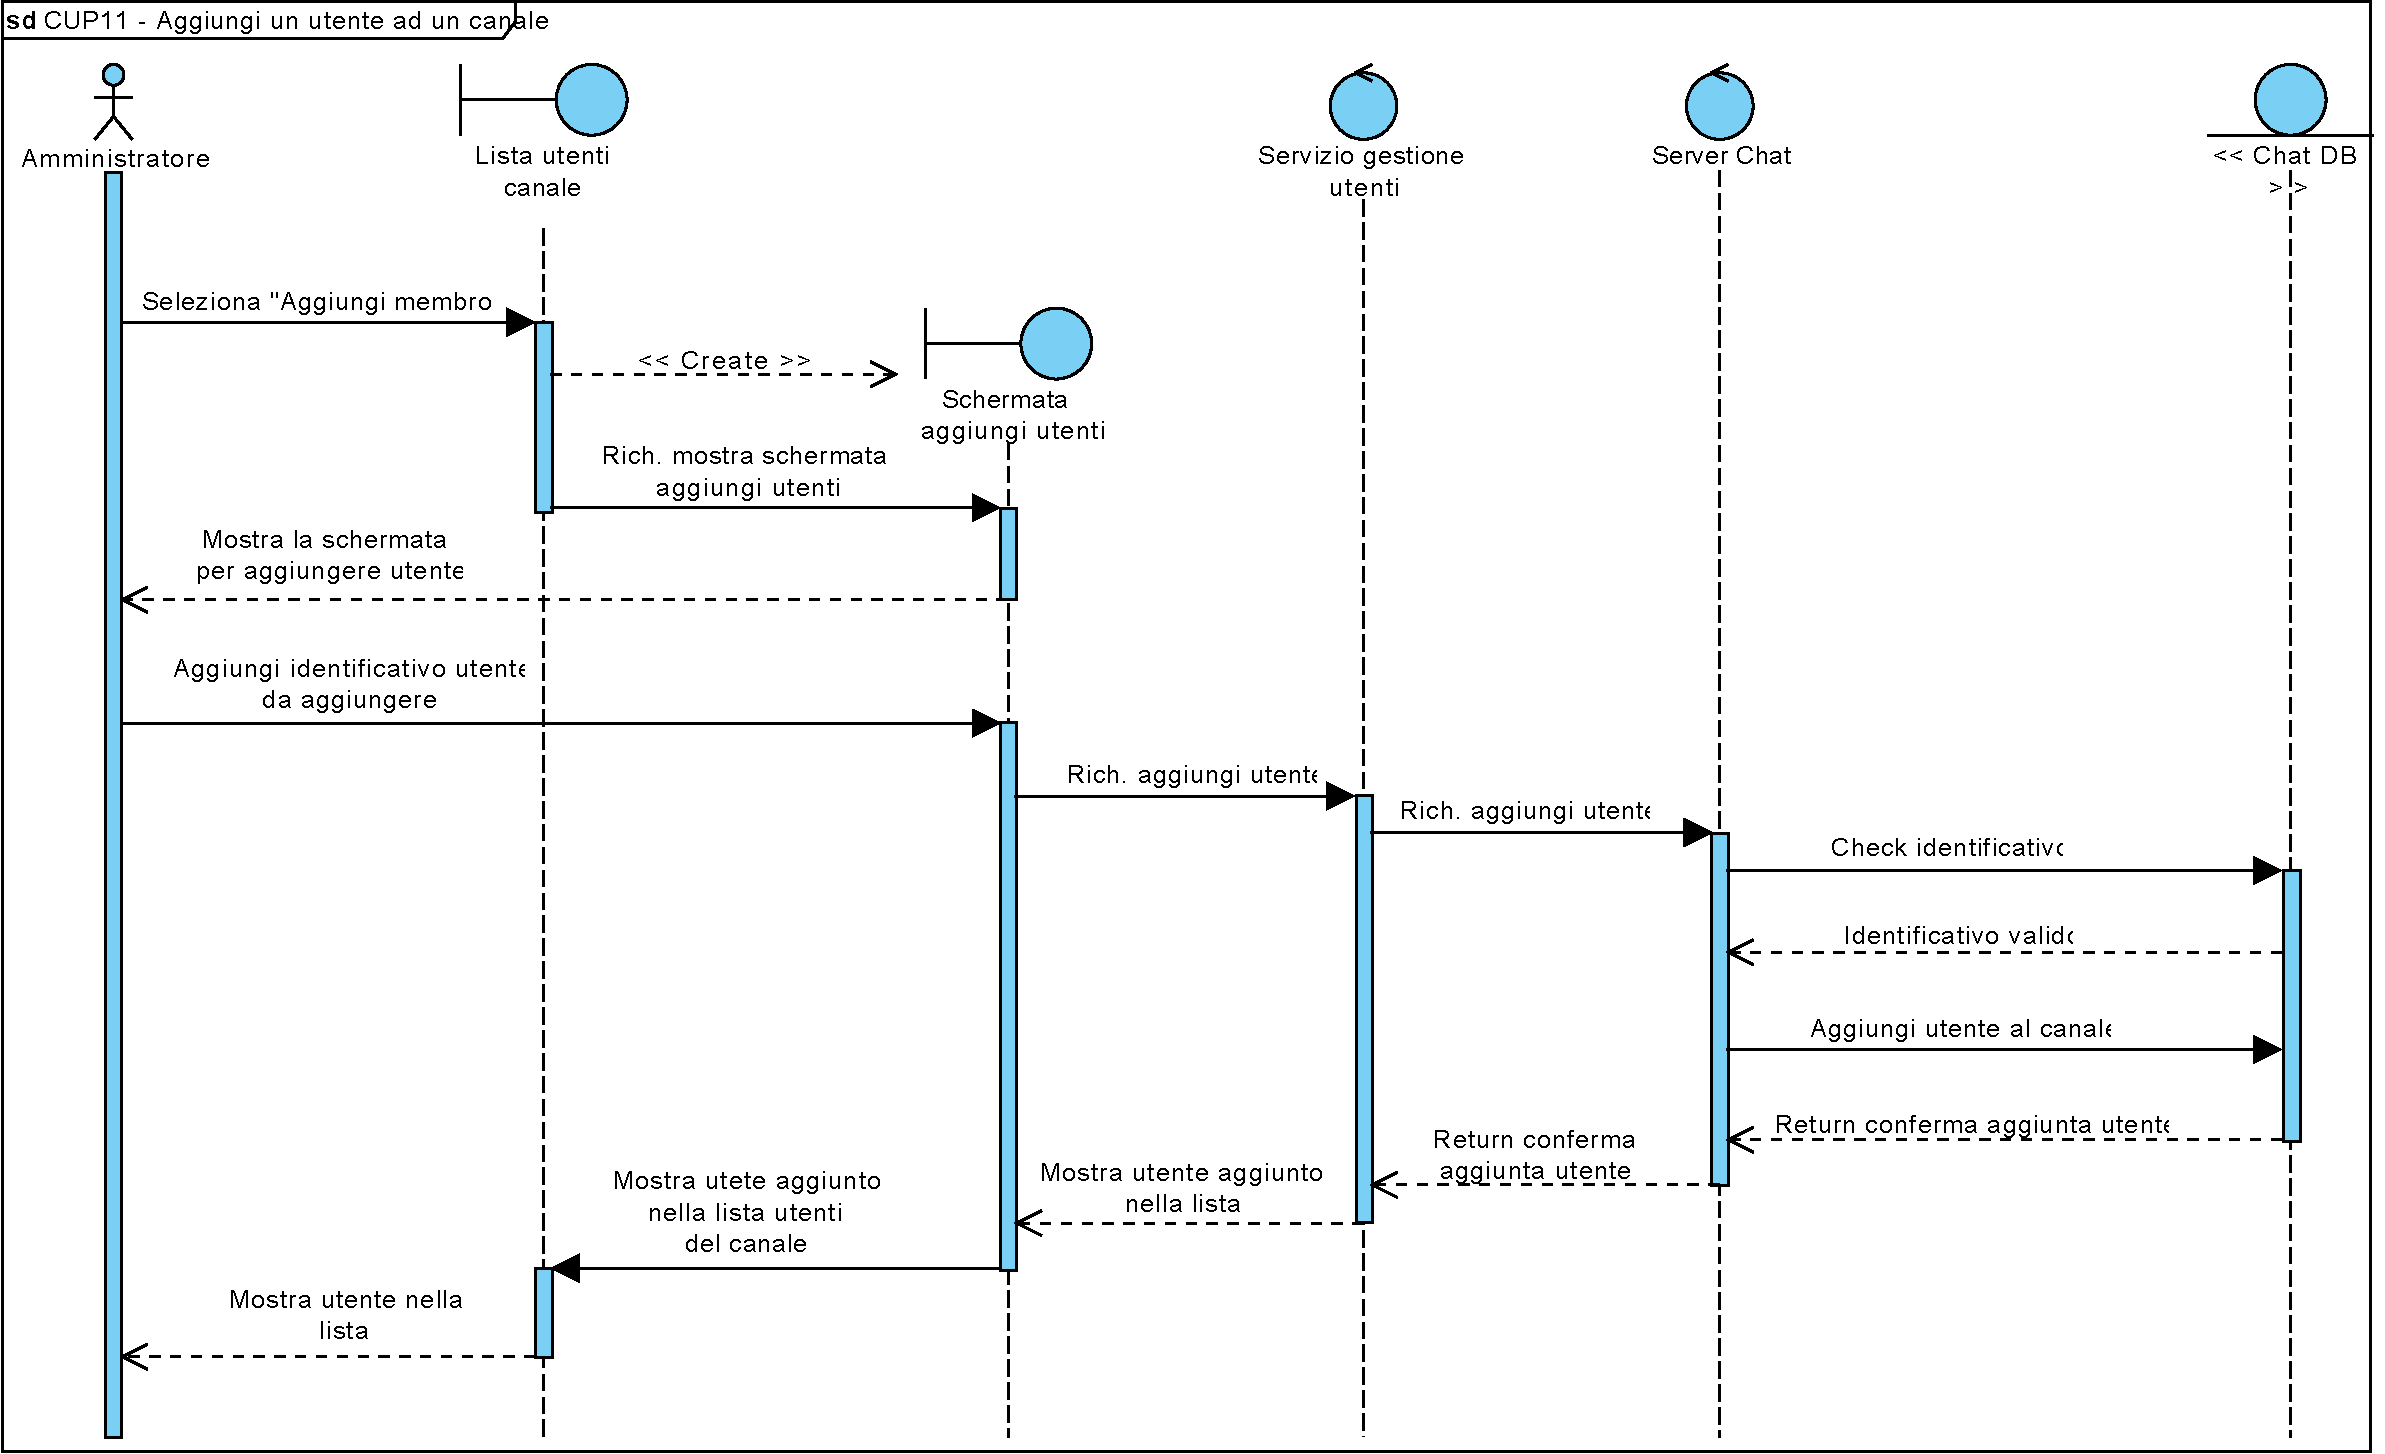
\includegraphics[height=3in,width=5in]{imgs/gruppo6/sequence/CUP11_aggiungi_un_utente_ad_un_canale.pdf}
	\caption{Aggiungi un utente ad un canale}
	\label{fig:prova}
\end{figure}

\begin{figure}
	\centering
	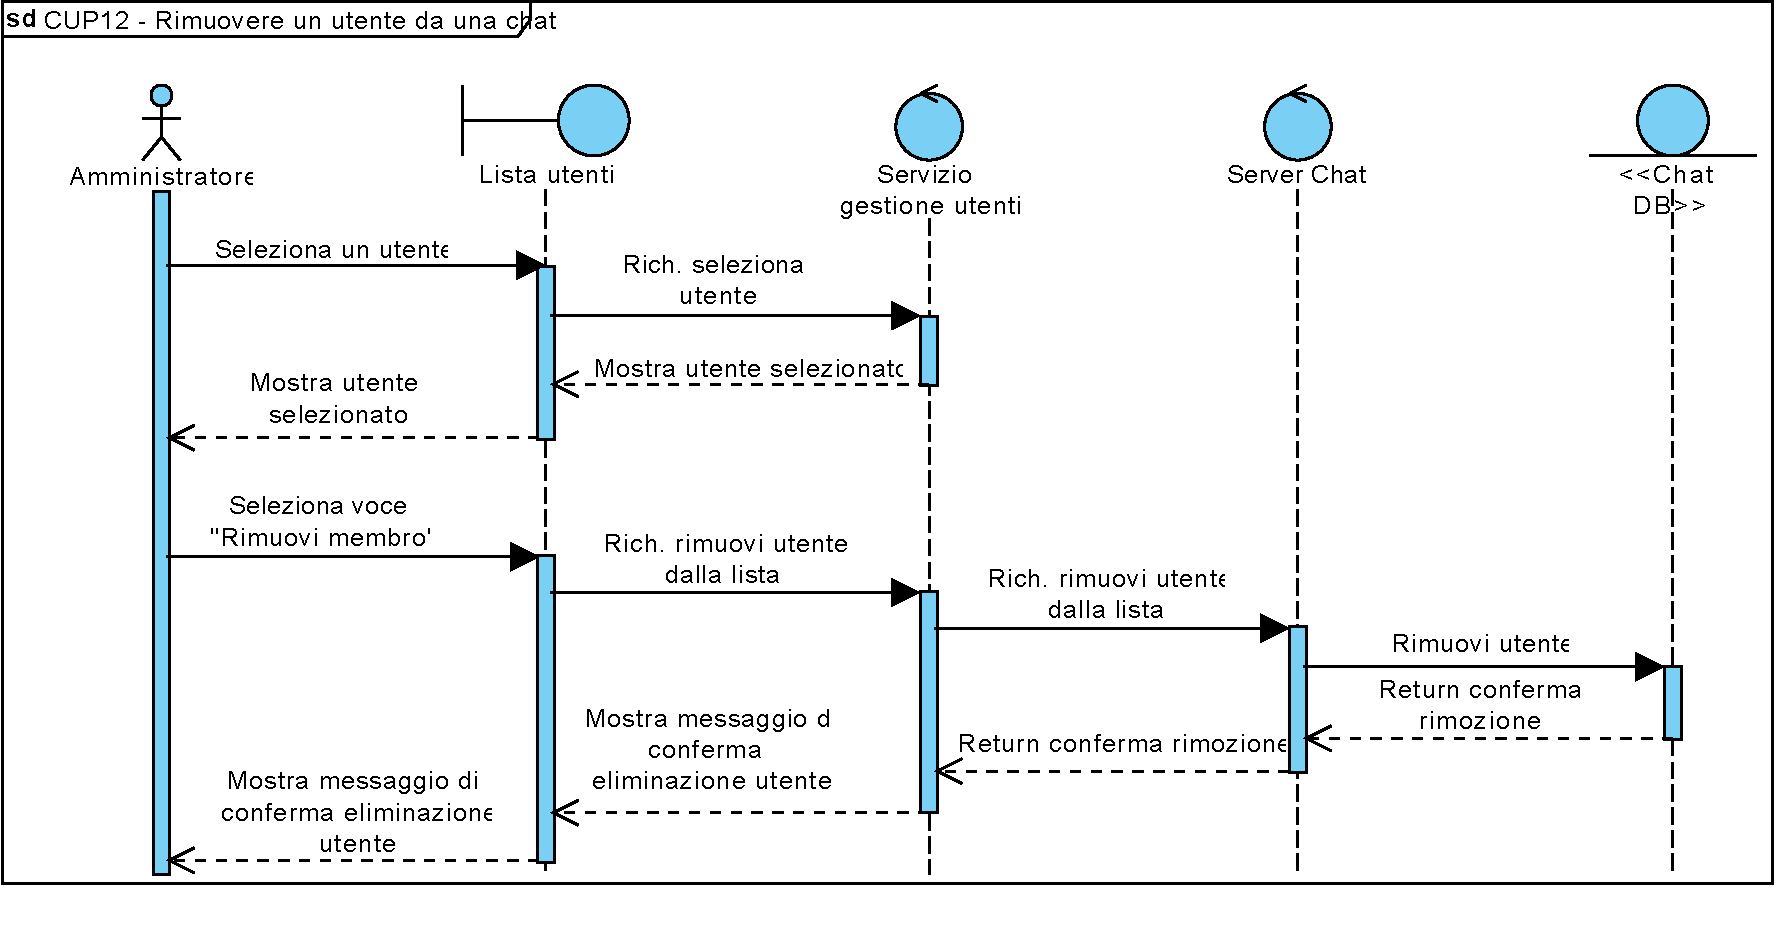
\includegraphics[height=3in,width=5in]{imgs/gruppo6/sequence/CUP12_rimuovere_un_utente_da_un_canale.pdf}
	\caption{Rimuovere un utente ad un canale}
	\label{fig:prova}
\end{figure}

\begin{figure}
	\centering
	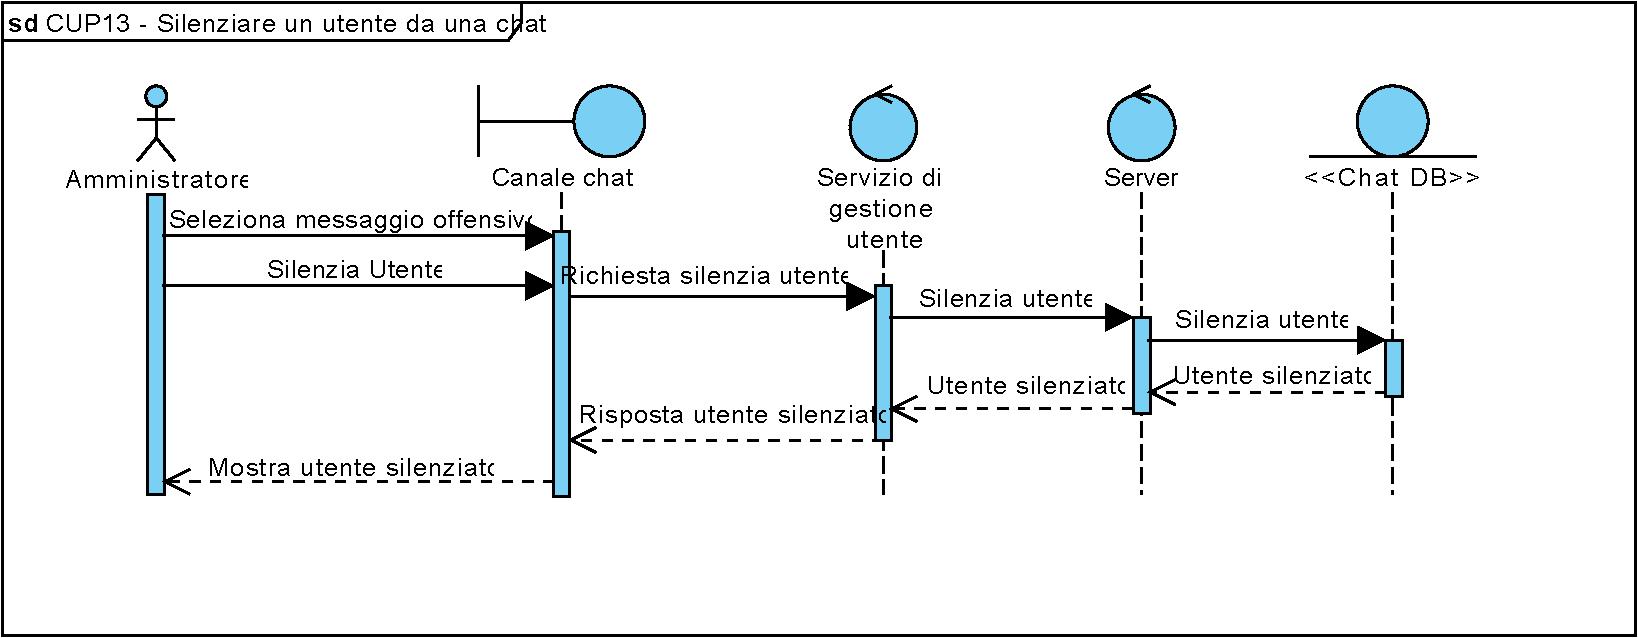
\includegraphics[height=3in,width=5in]{imgs/gruppo6/sequence/CUP13_silenzia_un_utente_da_una_chat.pdf}
	\caption{Silenzia un utente da una chat}
	\label{fig:prova}
\end{figure}

\begin{figure}
	\centering
	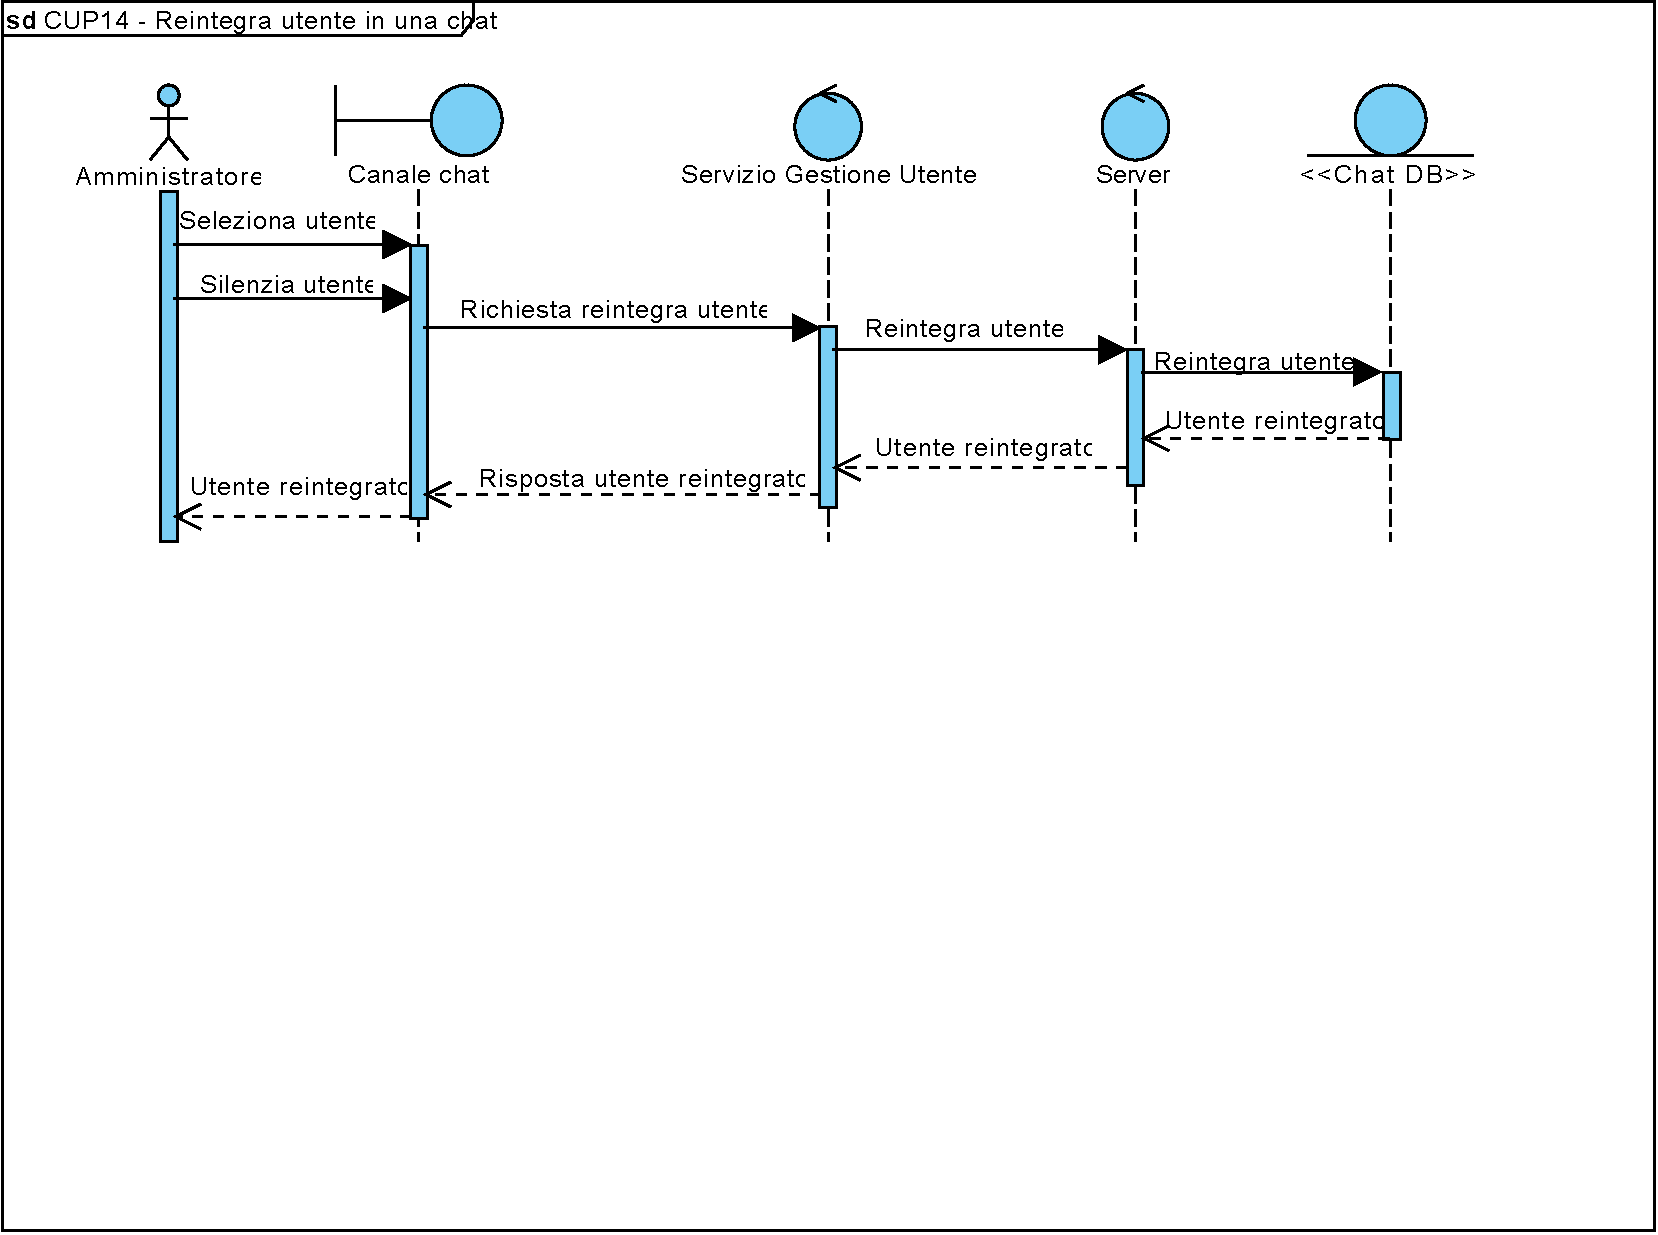
\includegraphics[height=3in,width=5in]{imgs/gruppo6/sequence/CUP14_reintegra_utente_in_una_chat.pdf}
	\caption{Reintegra utente in una chat}
	\label{fig:prova}
\end{figure}

\begin{figure}
	\centering
	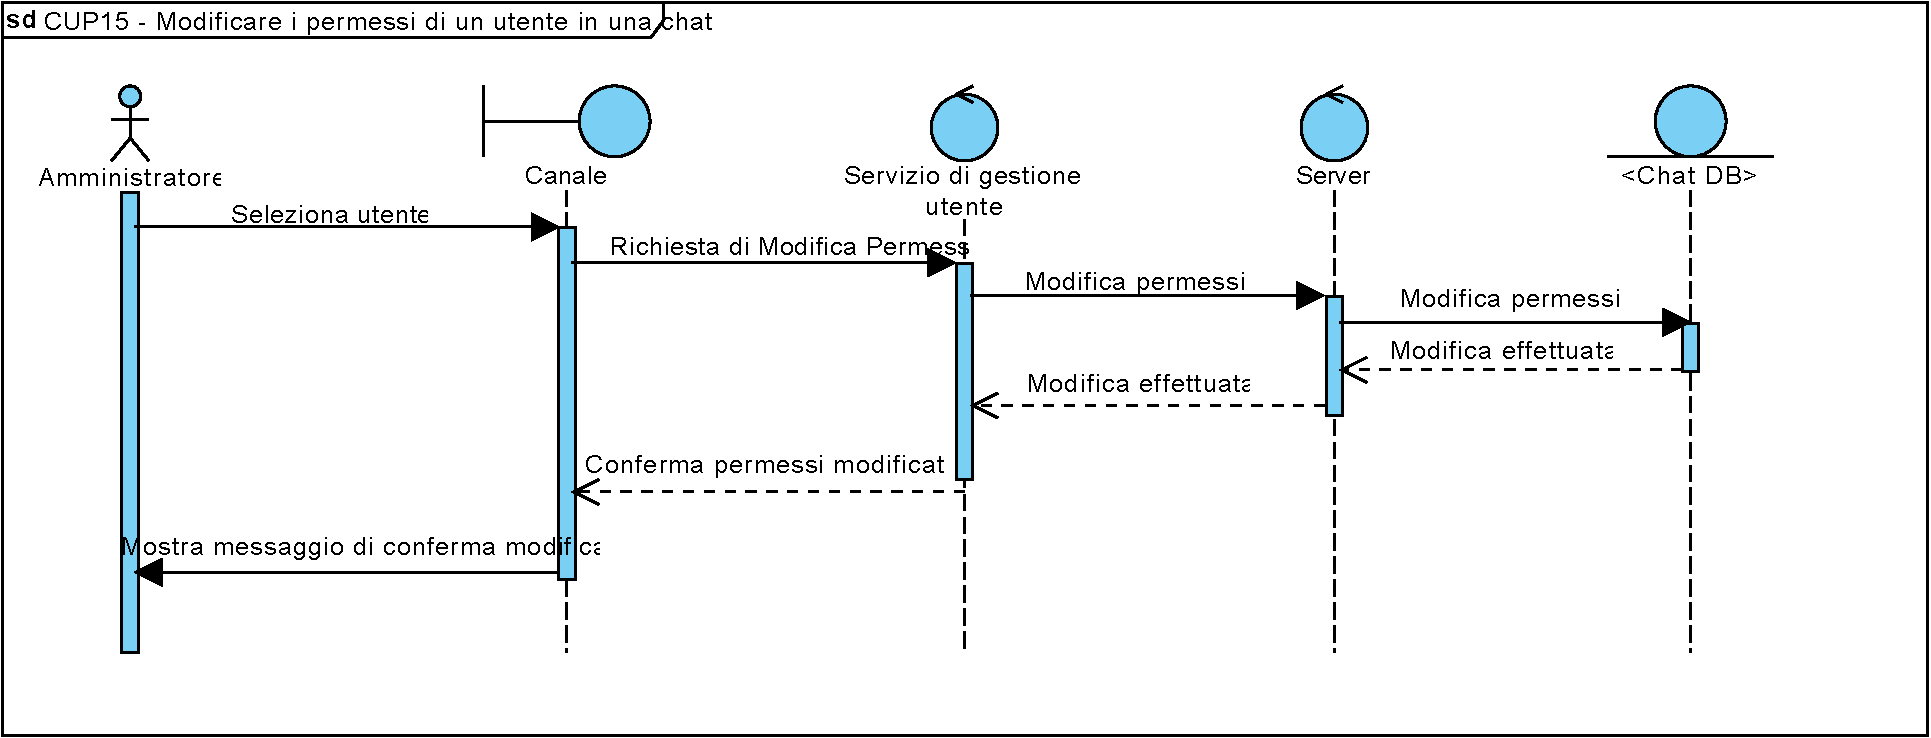
\includegraphics[height=3in,width=5in]{imgs/gruppo6/sequence/CUP15_modificare_i_permessi_di_un_utente.pdf}
	\caption{Modificare i permessi di un utente}
	\label{fig:prova}
\end{figure}

\begin{figure}
	\centering
	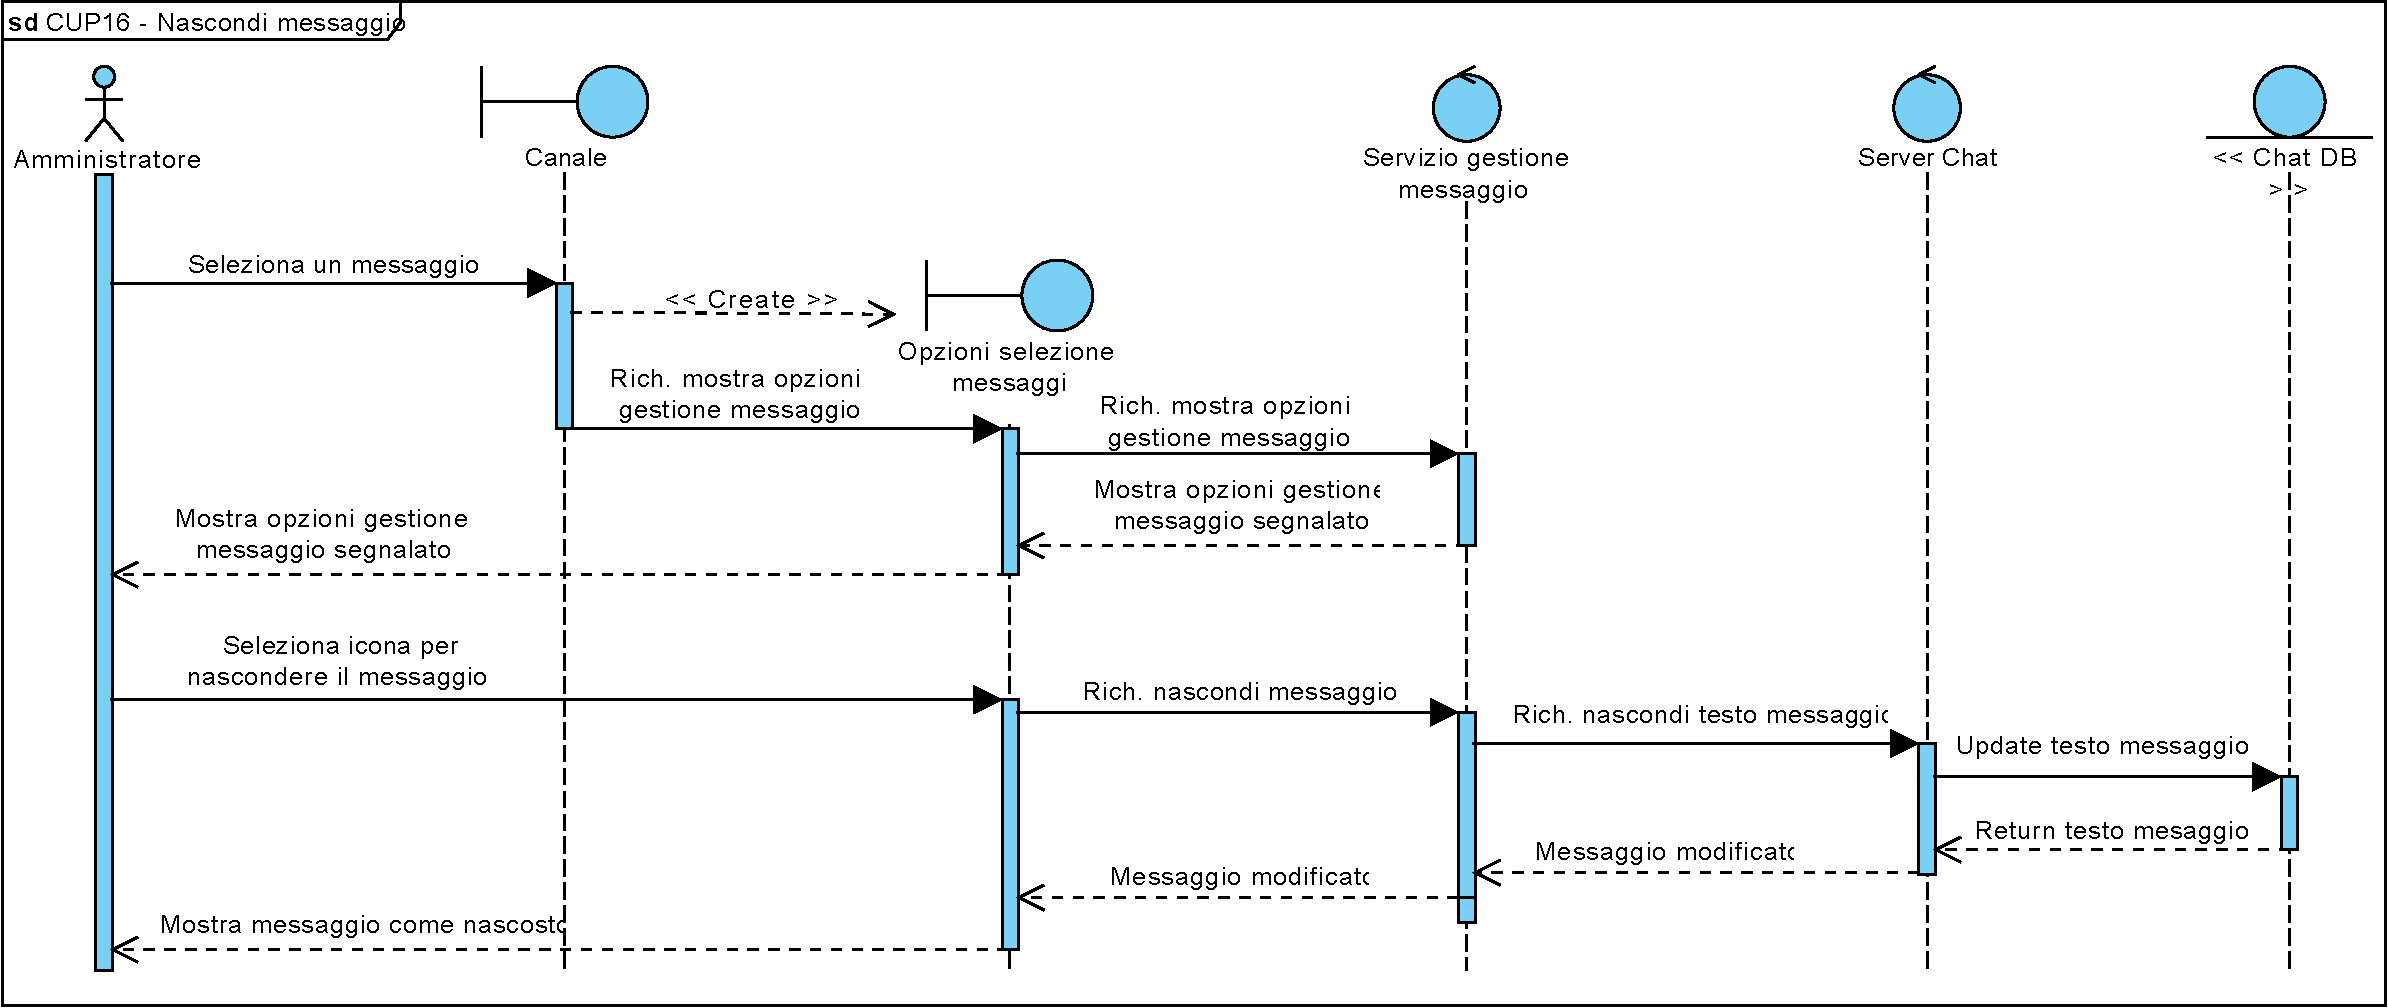
\includegraphics[height=3in,width=5in]{imgs/gruppo6/sequence/CUP16_nascondi_messaggio.pdf}
	\caption{Nascondi messaggio}
	\label{fig:prova}
\end{figure}

\begin{figure}
	\centering
	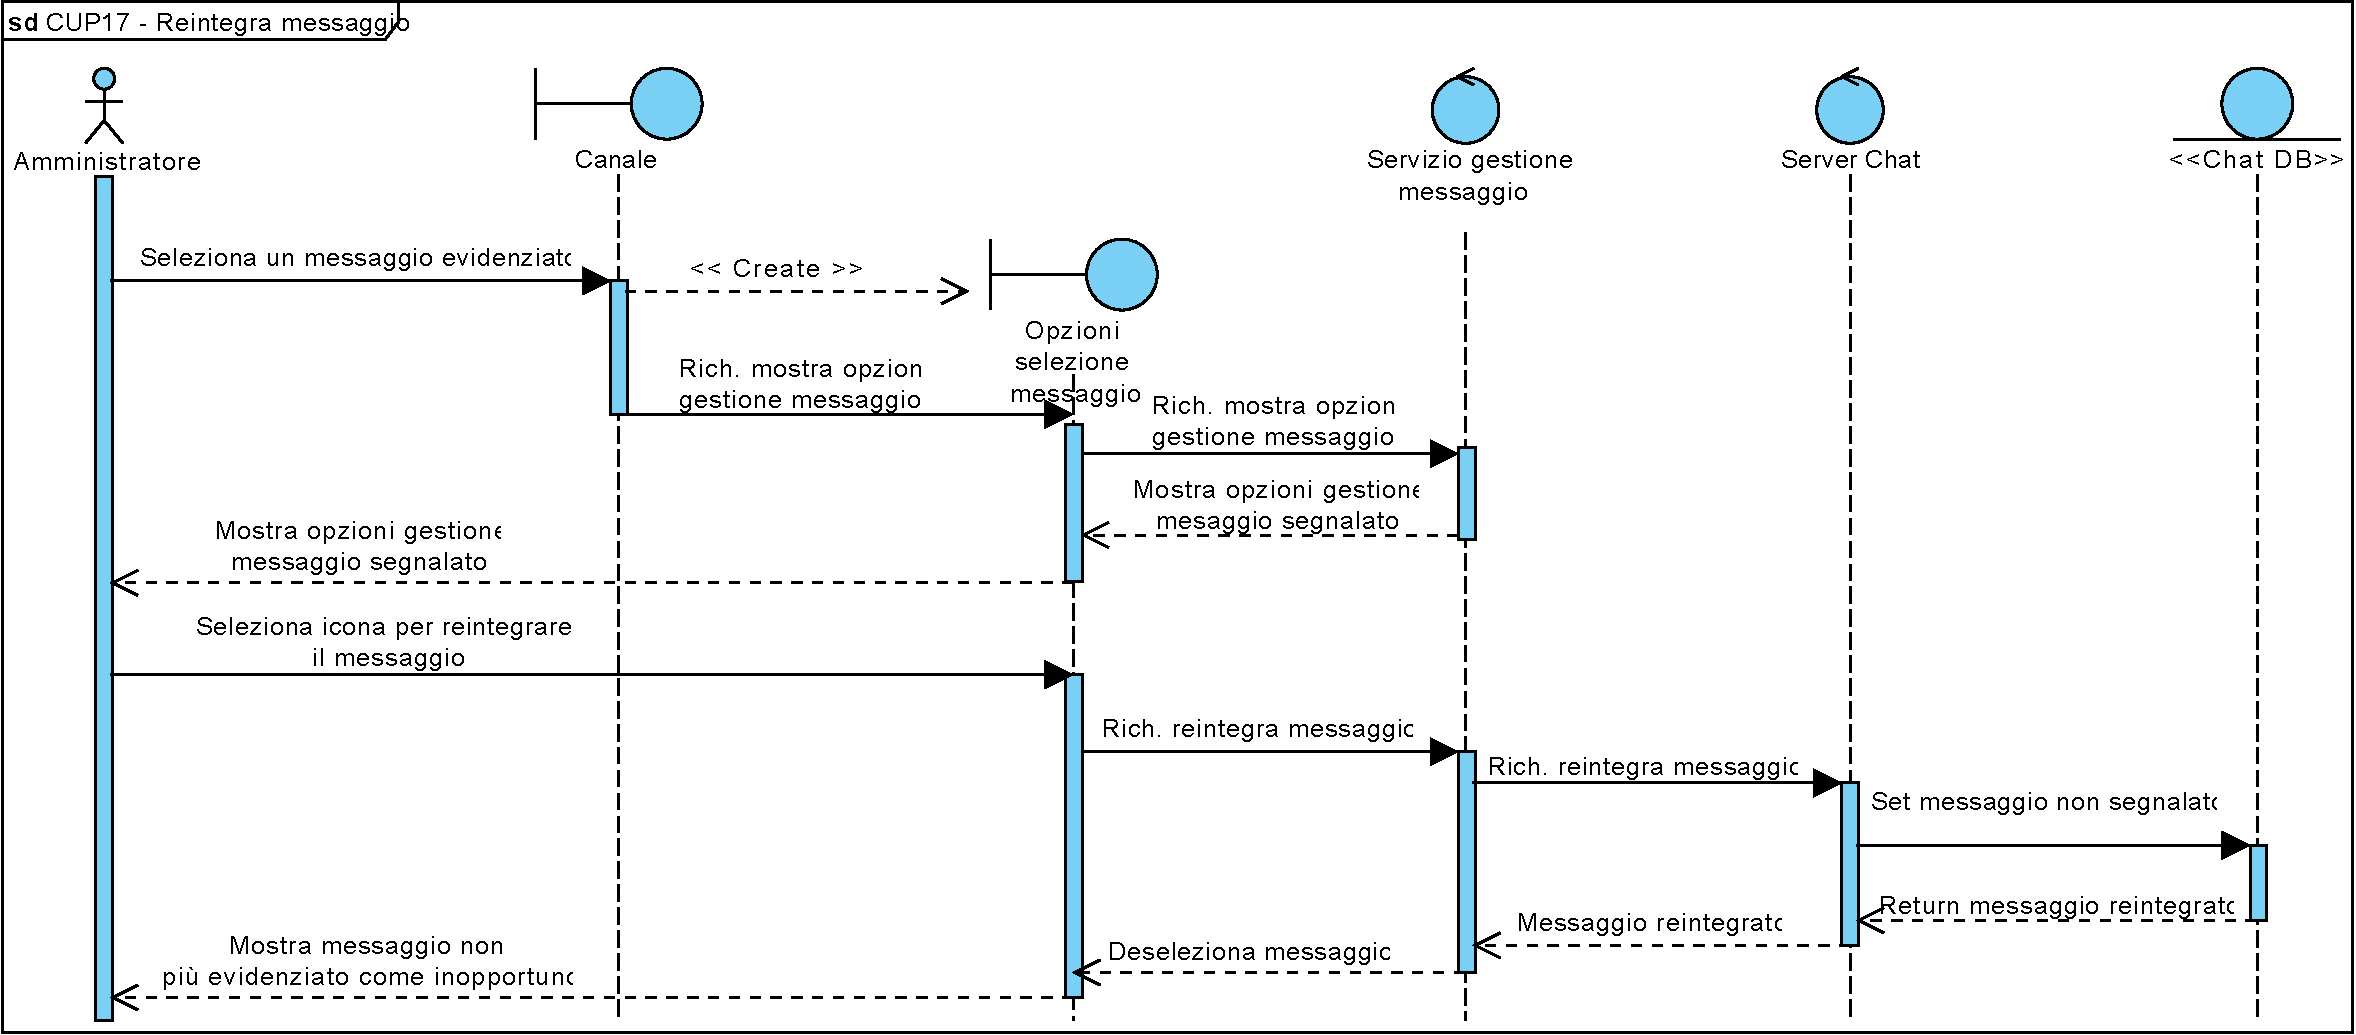
\includegraphics[height=3in,width=5in]{imgs/gruppo6/sequence/seq_cup17_reintegra_messaggio.pdf}
	\caption{Reintegra messaggio}
	\label{fig:seq-cup17}
\end{figure}

\begin{figure}
	\centering
	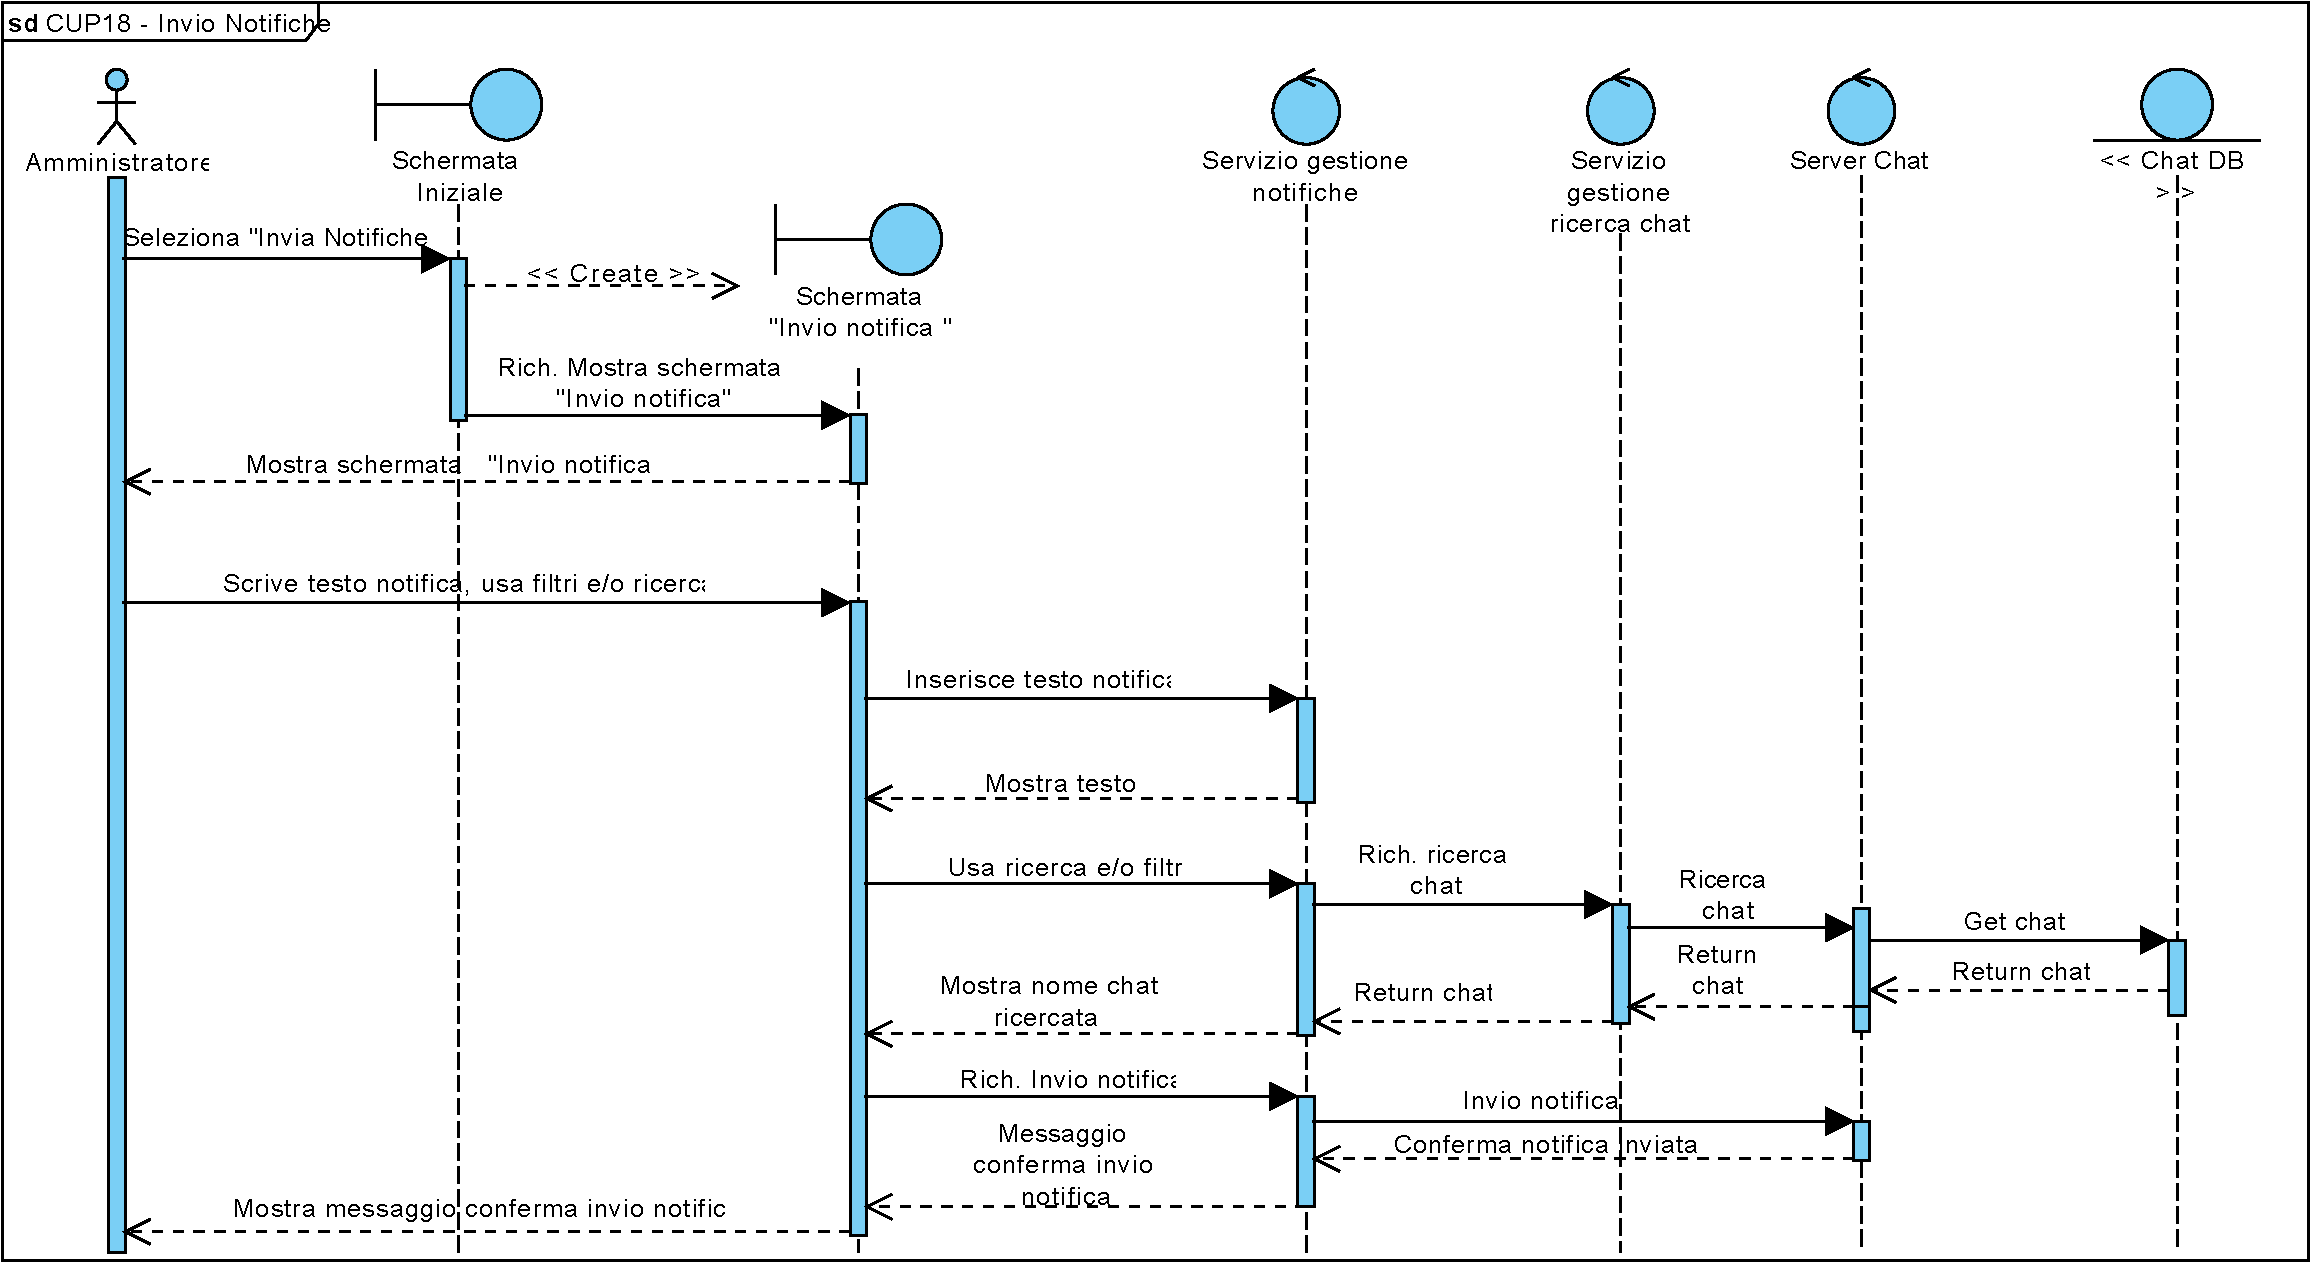
\includegraphics[height=3in,width=5in]{imgs/gruppo6/sequence/CUP18_invio_notifica.pdf}
	\caption{Invio notifica}
	\label{fig:prova}
\end{figure}


\begin{figure}
	\centering
	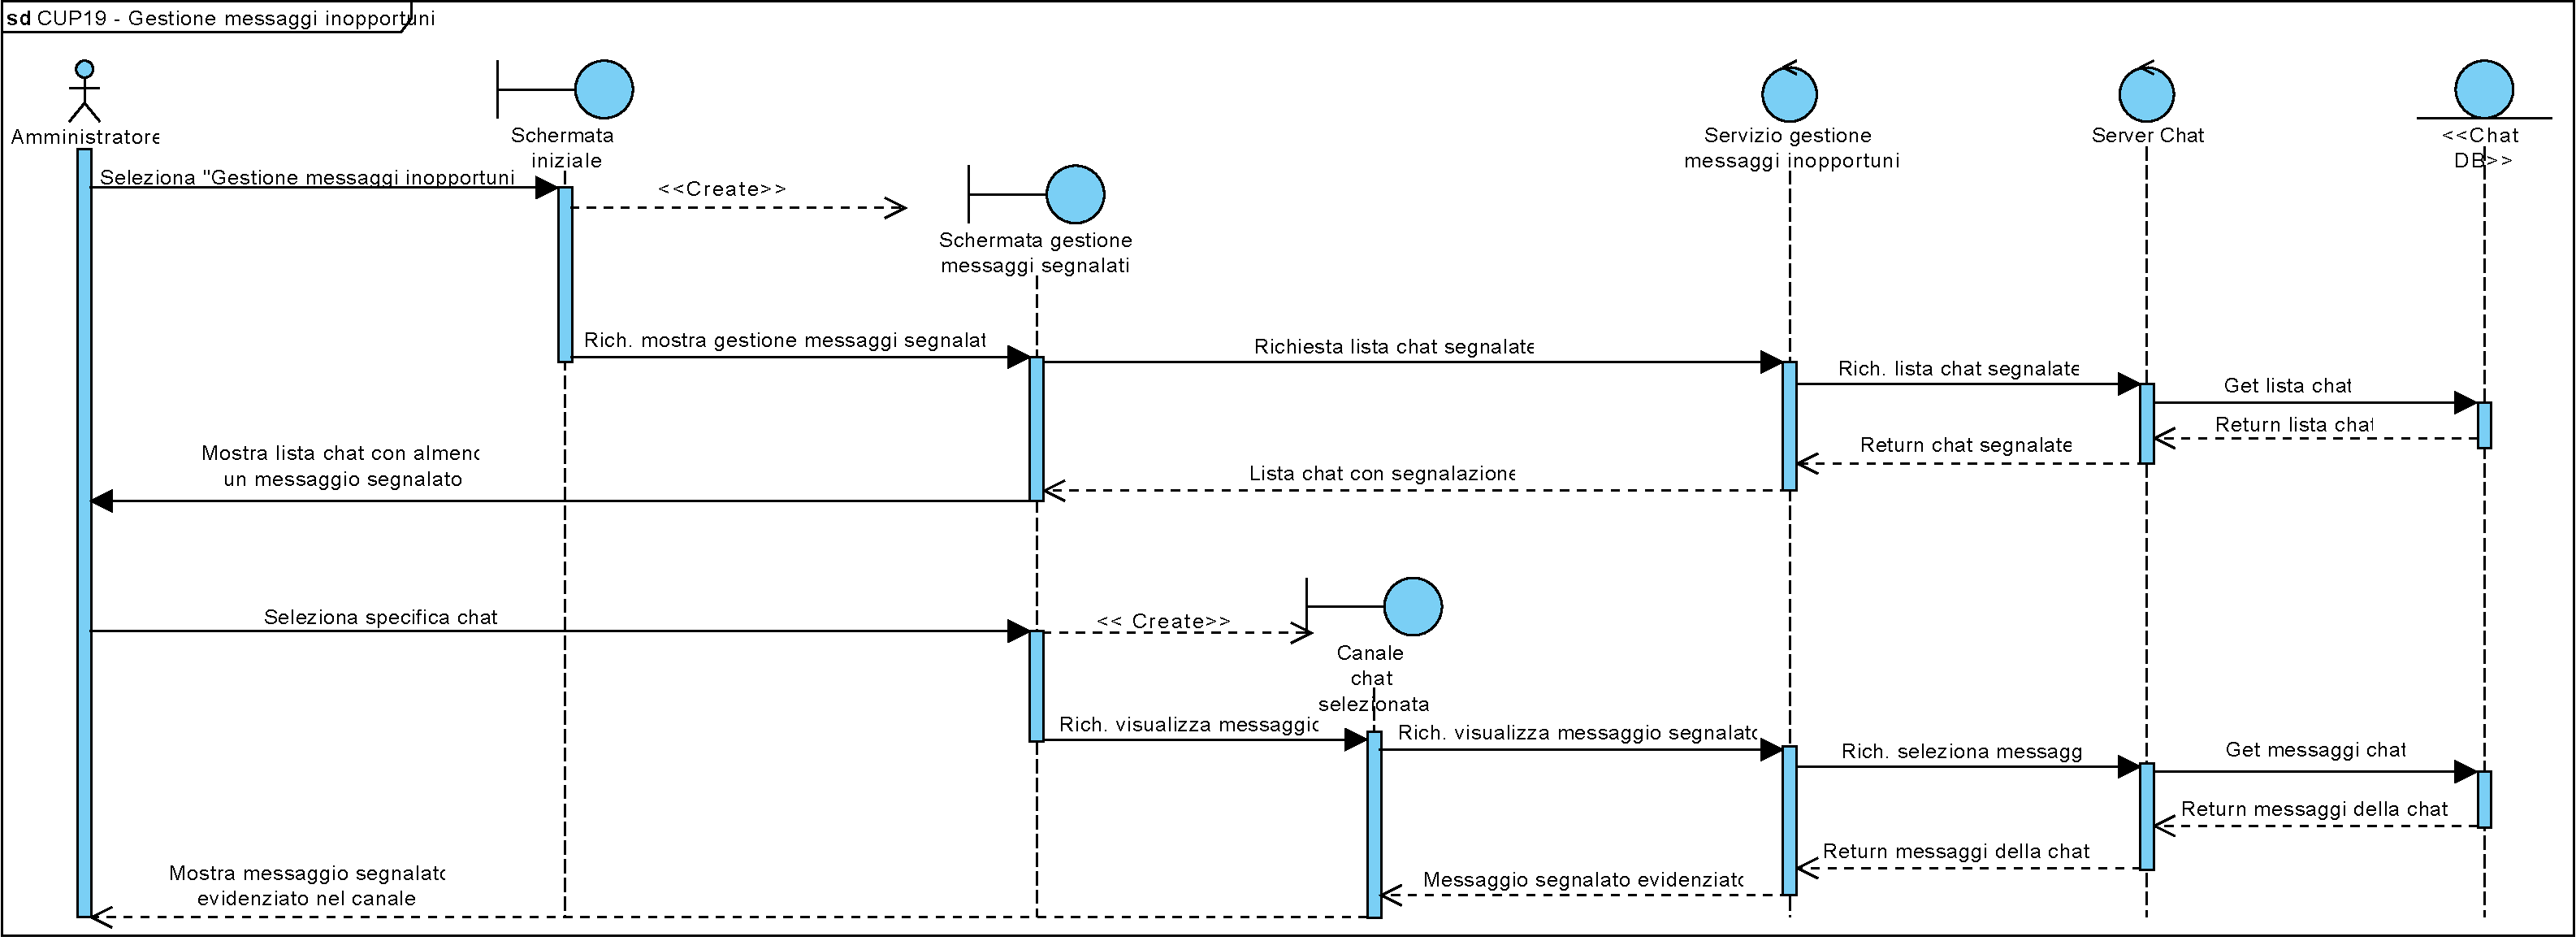
\includegraphics[height=3in,width=5in]{imgs/gruppo6/sequence/CUP19_gestione_messaggi_inopportuni.pdf}
	\caption{Gestione messaggi inopportuni}
	\label{fig:prova}
\end{figure}

\section{Diagramma delle attività}
%%% START activities chat studenti %%%
\begin{figure}
\subsection{Activities relative alla chat dell'App Studenti}
	\centering
	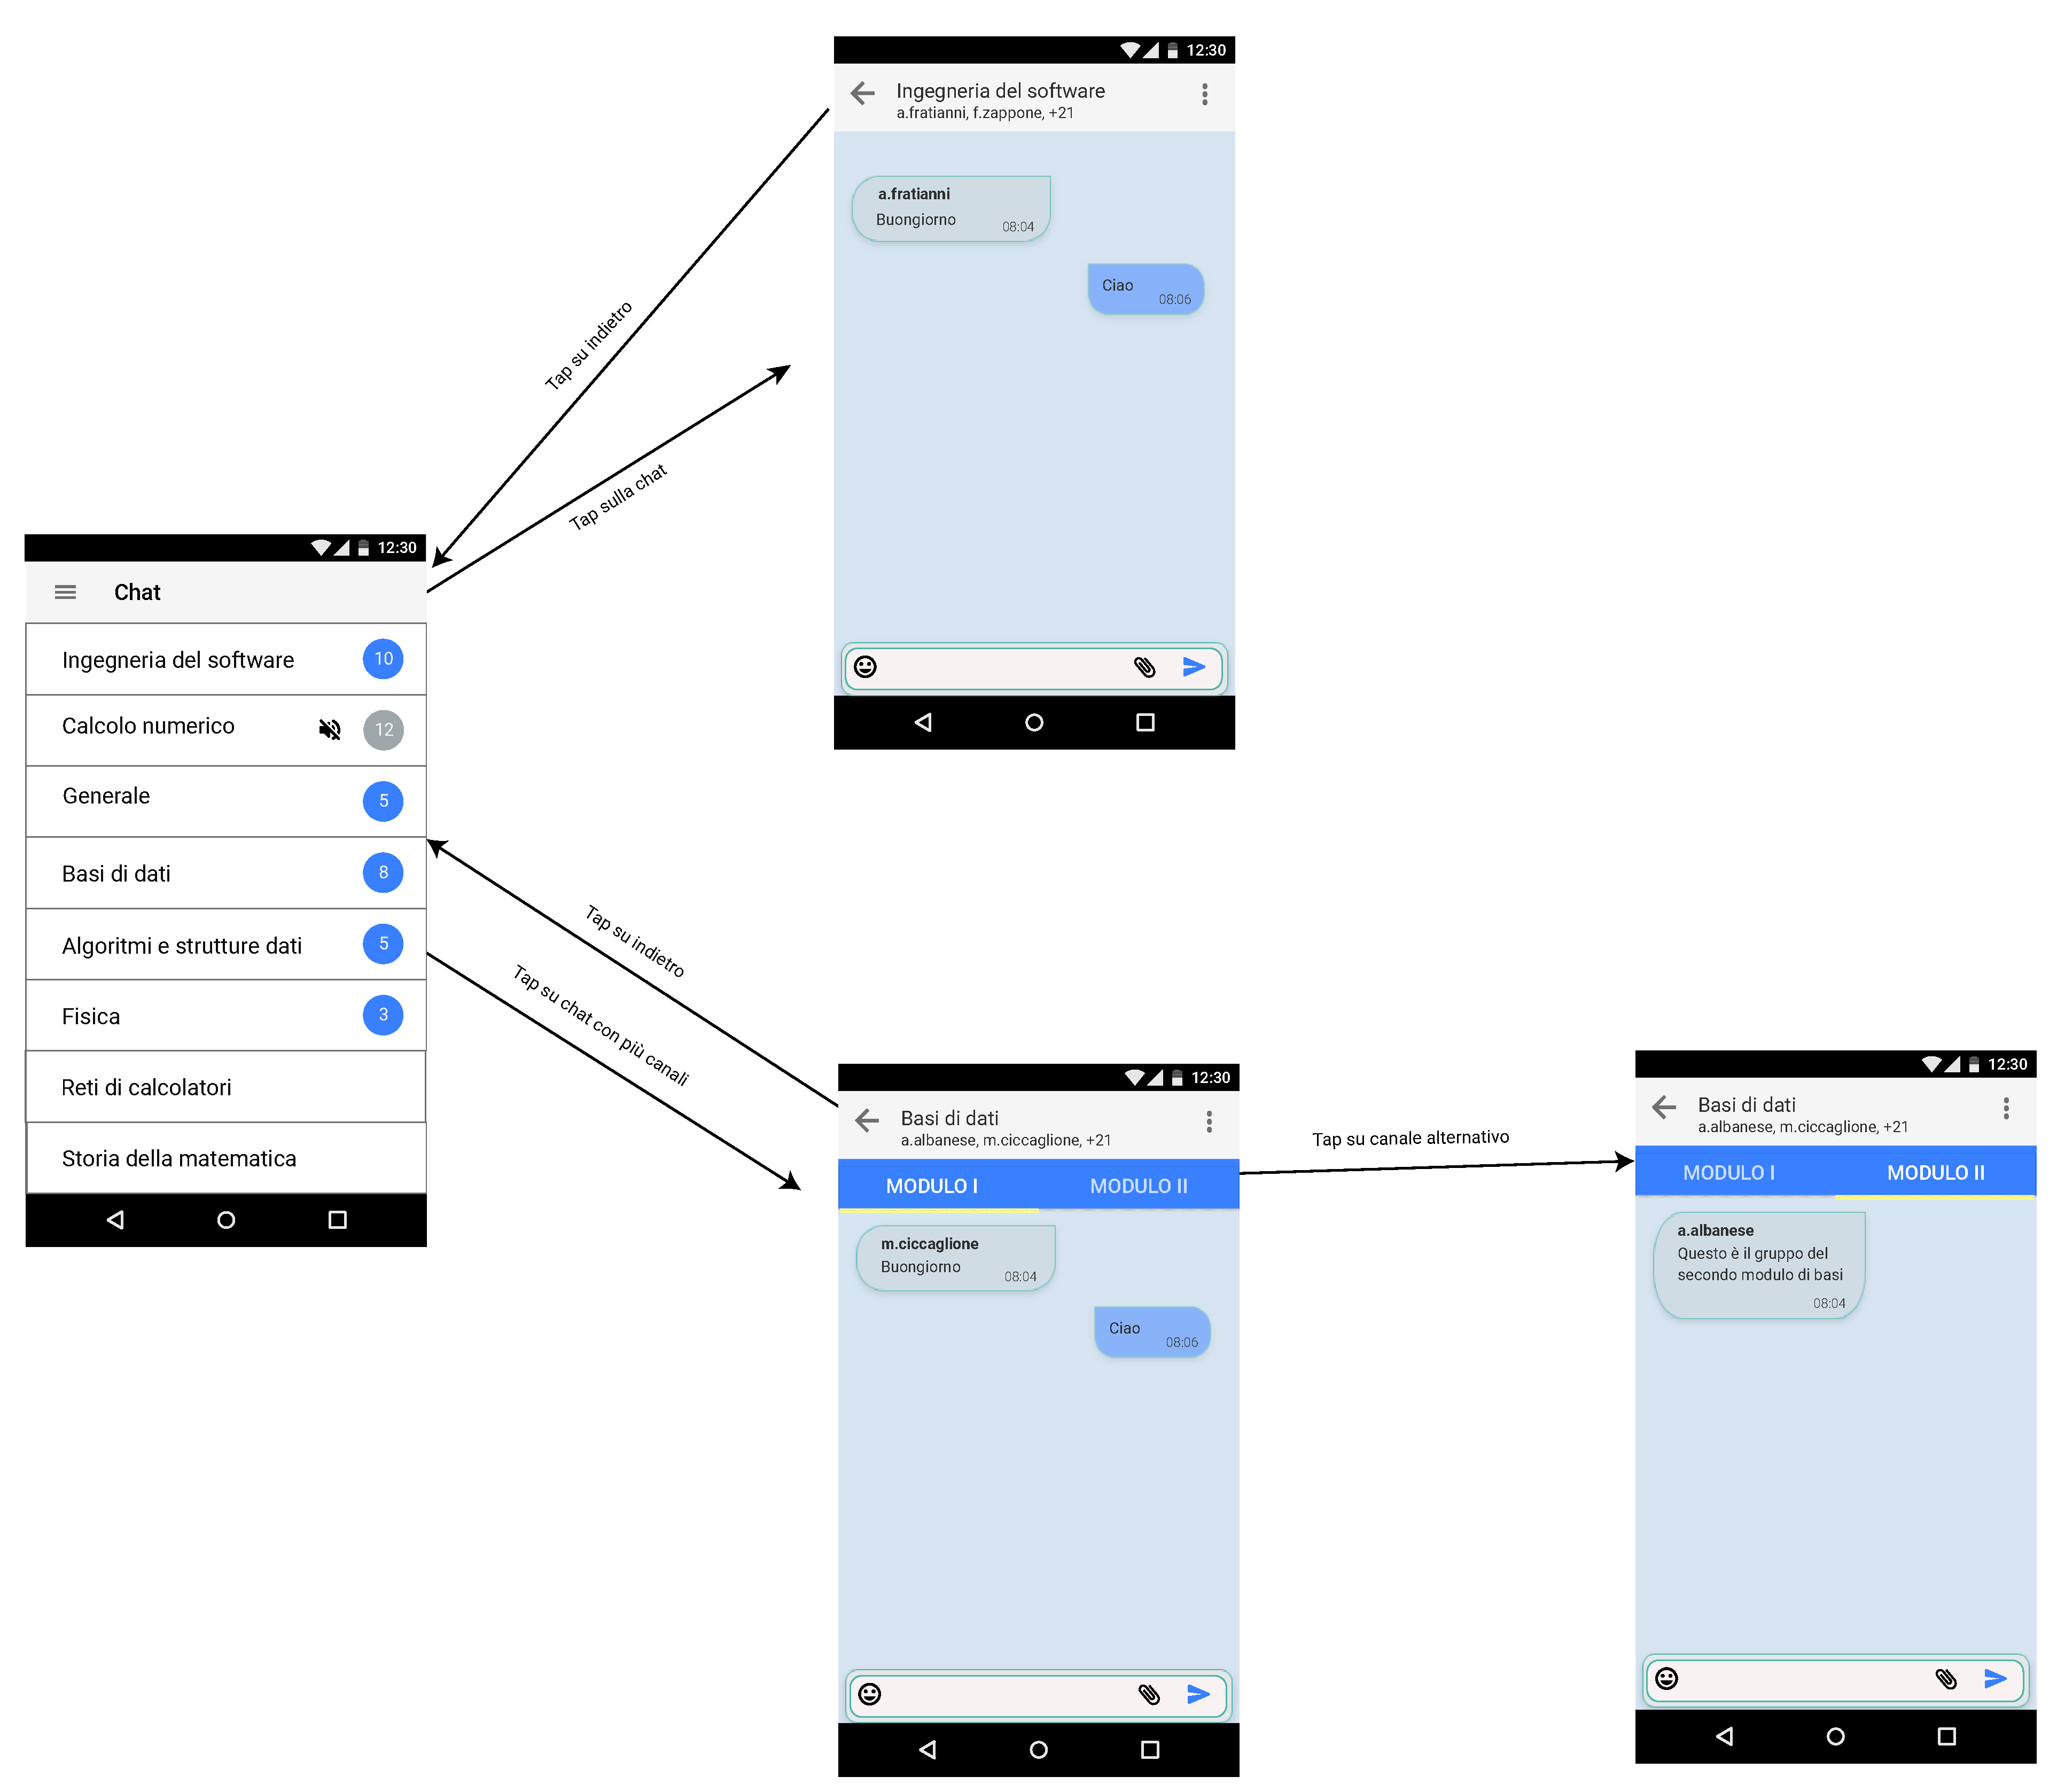
\includegraphics[width=0.9\textwidth]{imgs/gruppo6/activities/act_cus1_visualizza_canale.pdf}
	\caption{CUS 1 - Visualizza canale}
	\label{fig:cus1}
\end{figure}

\begin{figure}
	\centering
	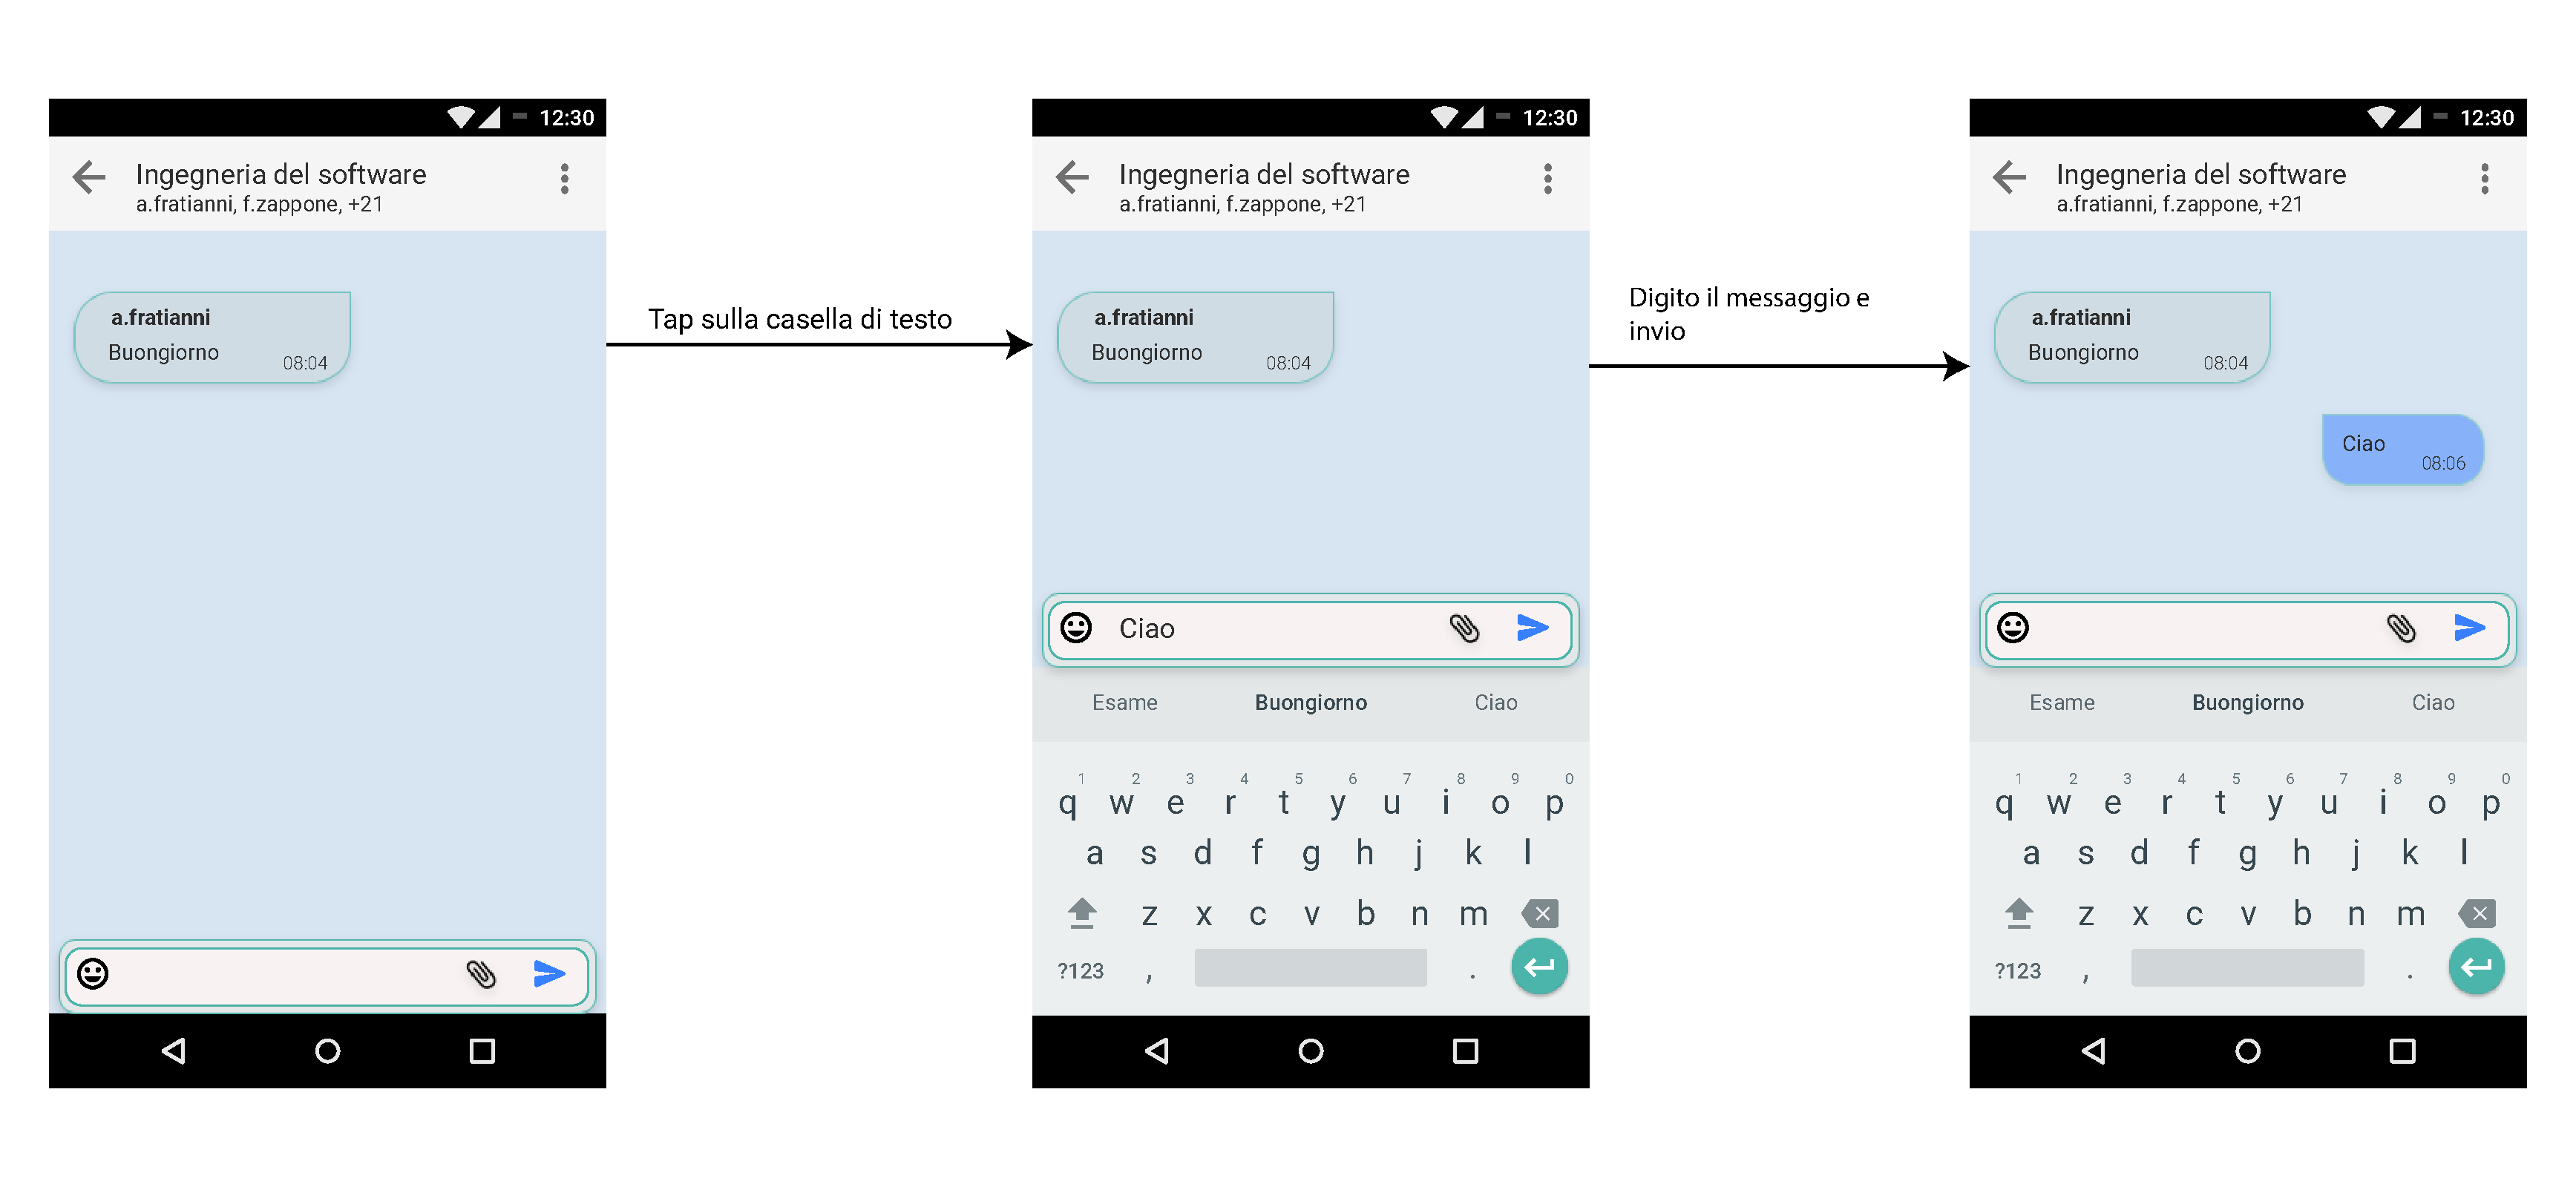
\includegraphics[width=0.9\textwidth]{imgs/gruppo6/activities/act_cus2_invio_messaggio.pdf}
	\caption{CUS2 - Invio messaggio}
	\label{fig:cus2}
\end{figure}

\begin{figure}
	\centering
	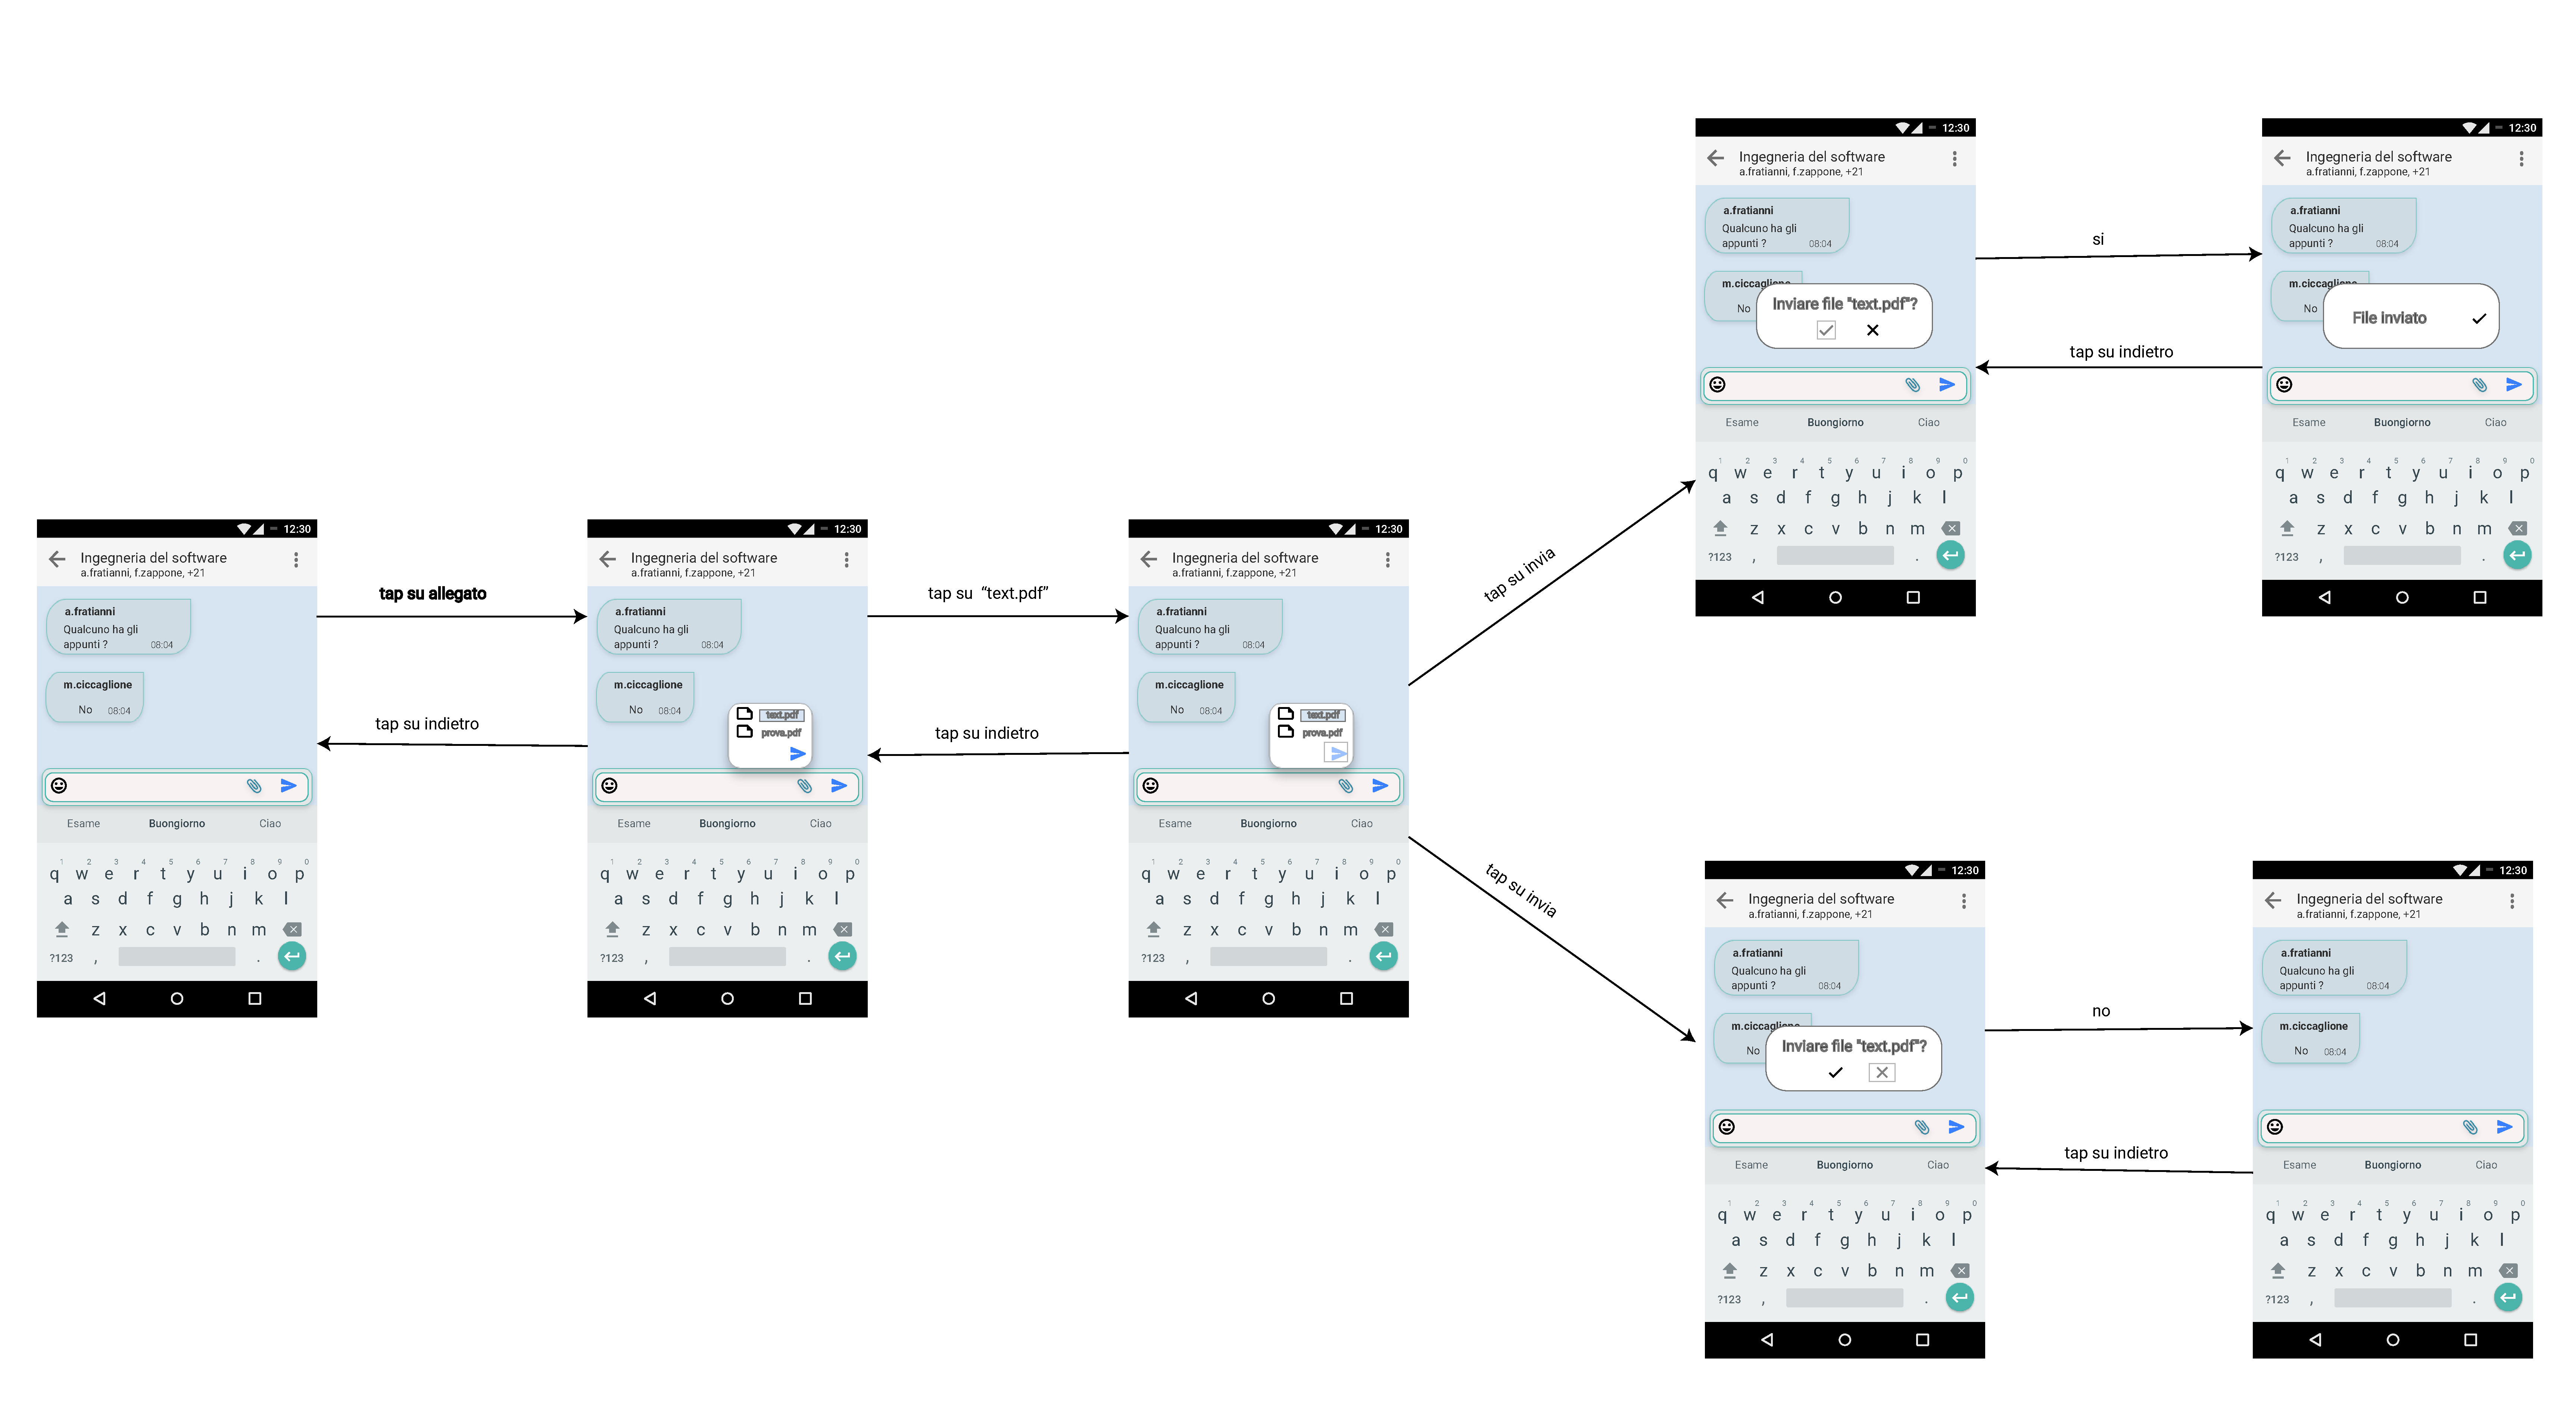
\includegraphics[width=0.9\textwidth]{imgs/gruppo6/activities/act_cus3_invia_allegato.pdf}
	\caption{CUS3 - Invio Allegato}
	\label{fig:cus3-1}
\end{figure}

\begin{figure}
	\centering
	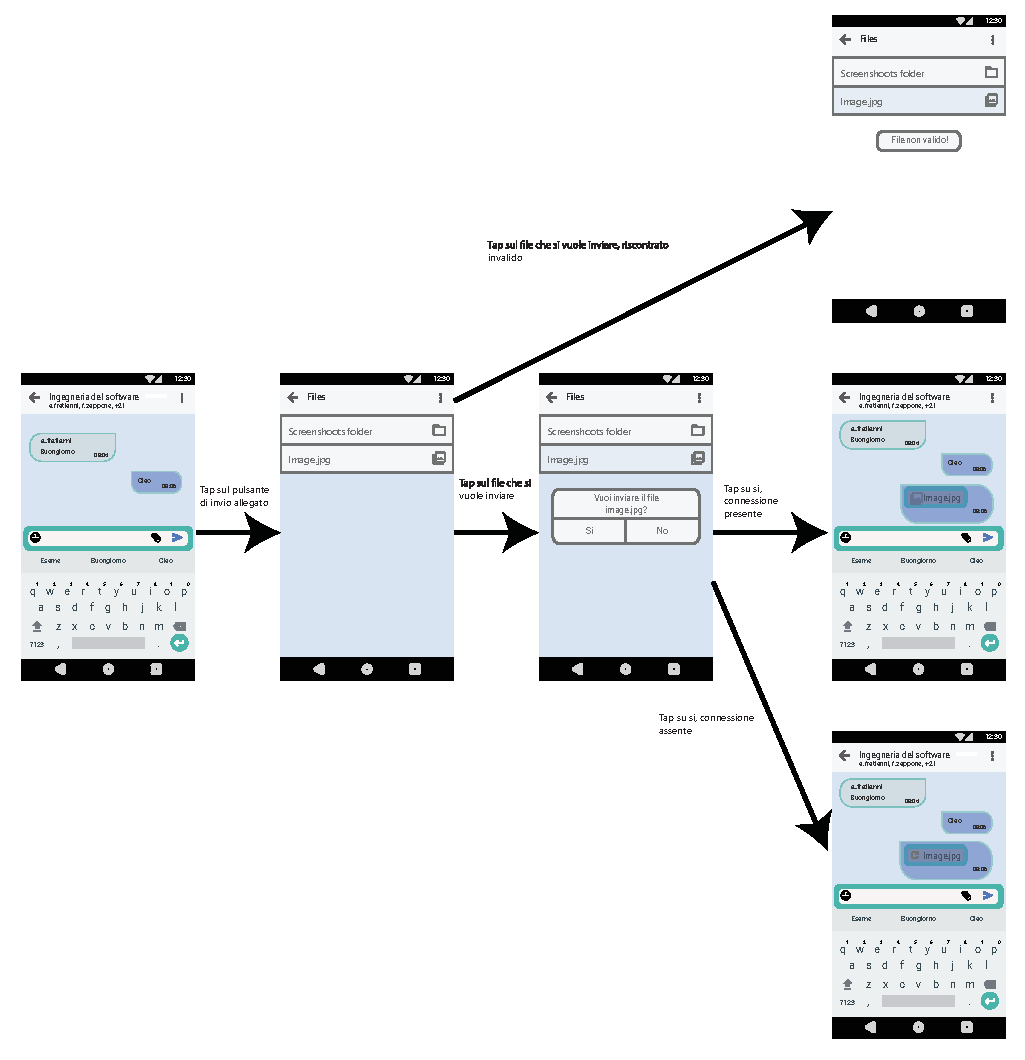
\includegraphics[width=0.9\textwidth]{imgs/gruppo6/activities/act_cus3_invio_allegato2.pdf}
	\caption{CUS3 - Invio Allegato (es. 2)}
	\label{fig:cus3-2}
\end{figure}

\begin{figure}
	\centering
	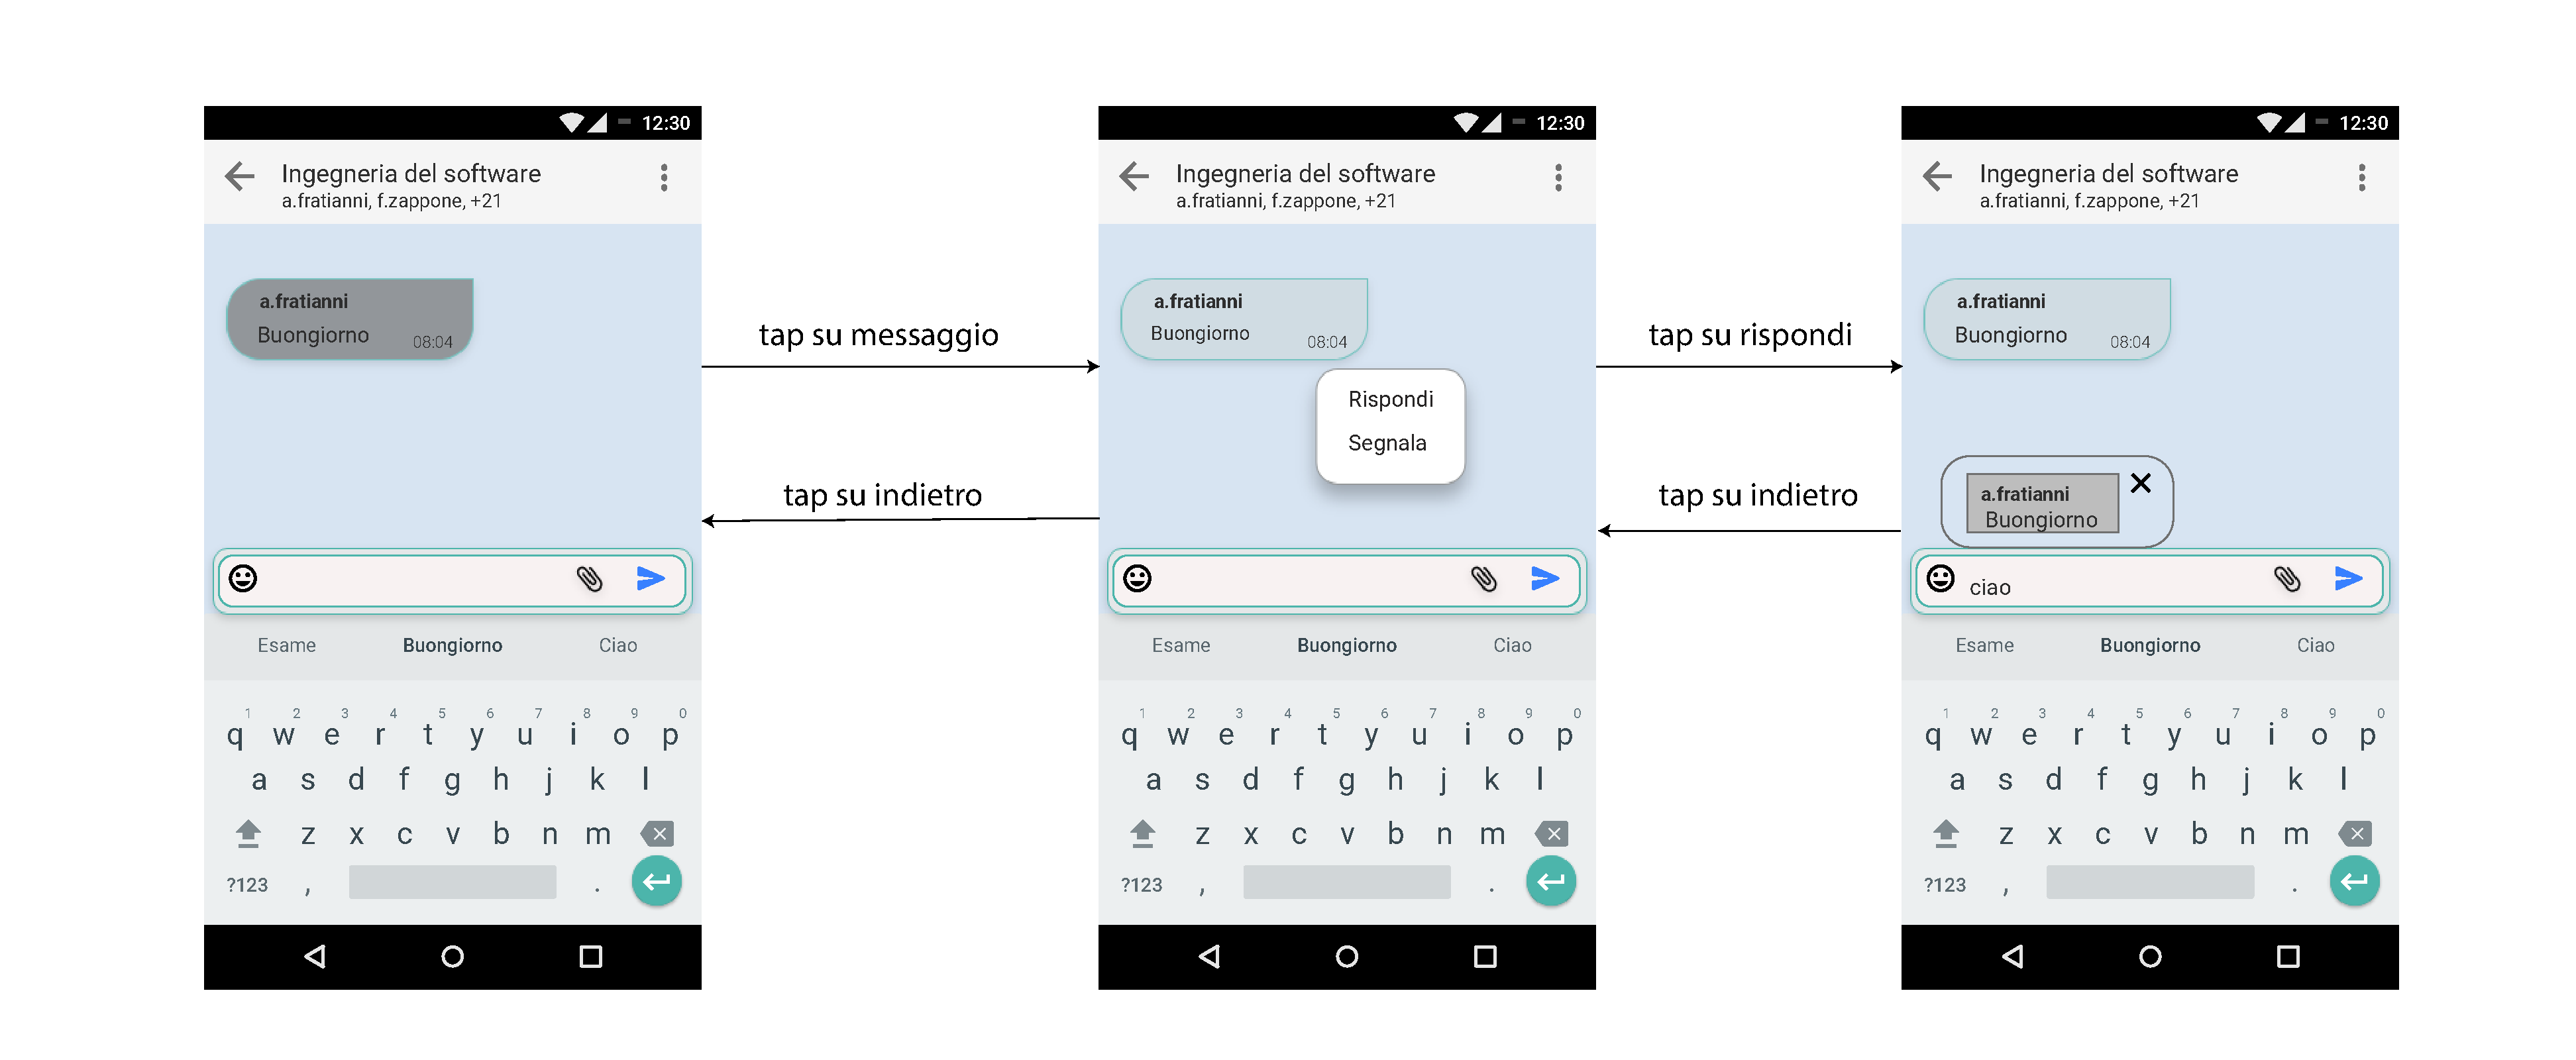
\includegraphics[width=0.9\textwidth]{imgs/gruppo6/activities/act_cus4_rispondi_singolo_messaggio.pdf}
	\caption{CUS4 - Rispondi al messaggio}
	\label{fig:cus4}
\end{figure}

\begin{figure}
	\centering
	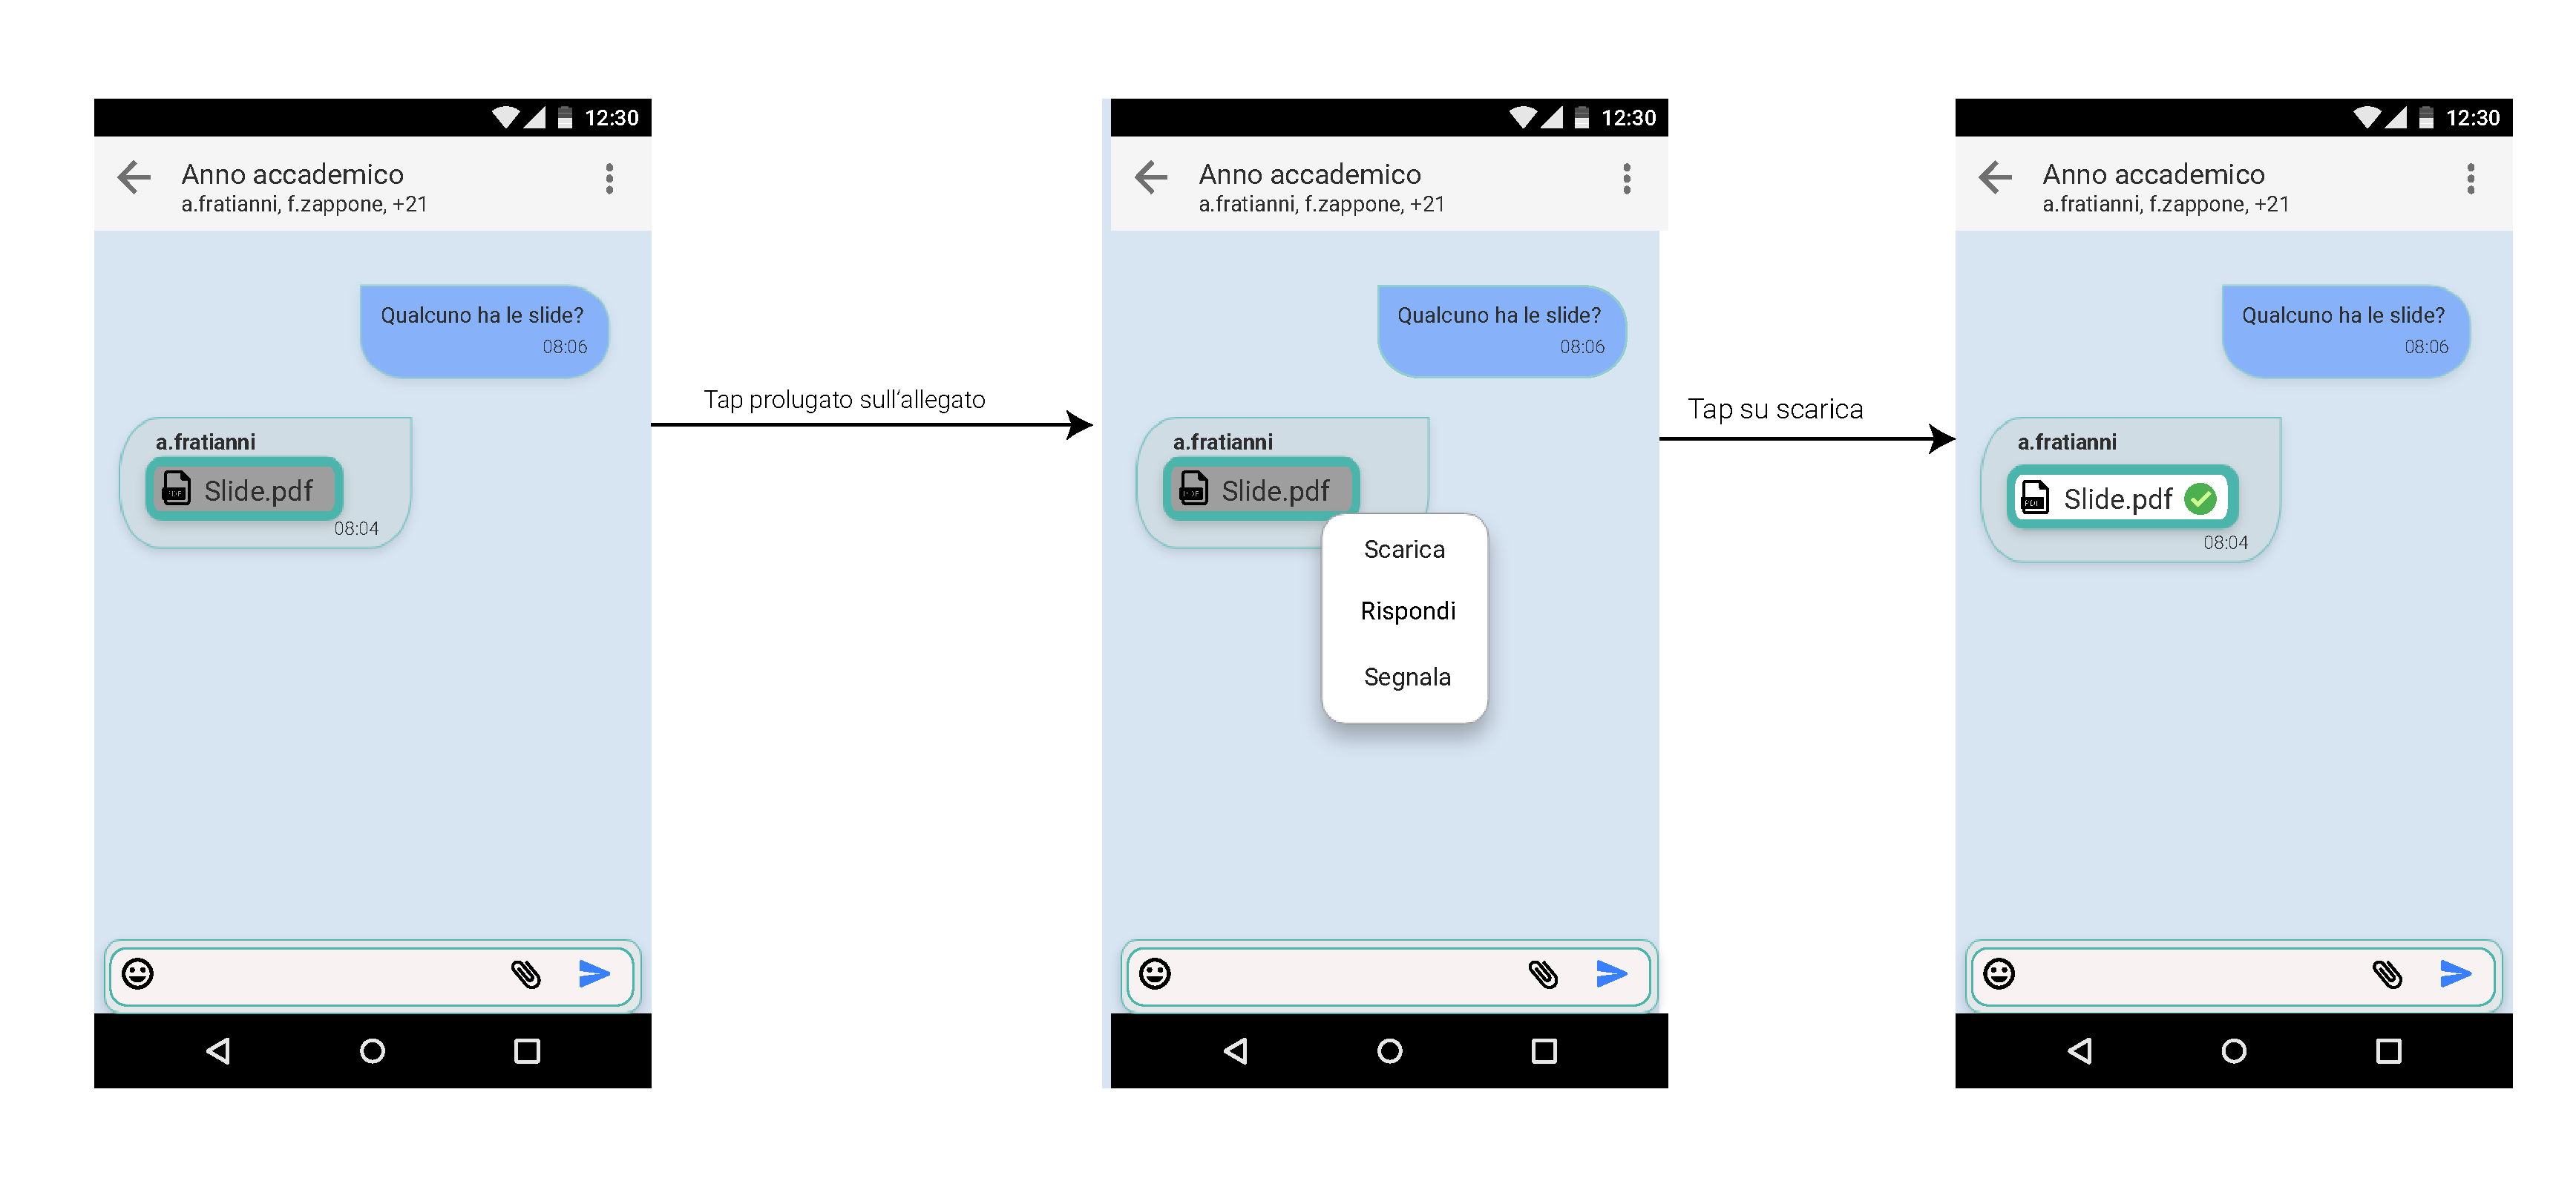
\includegraphics[width=0.9\textwidth]{imgs/gruppo6/activities/act_cus5_scarica_allegato.pdf}
	\caption{CUS5 - Scarica allegato}
	\label{fig:cus5}
\end{figure}

\begin{figure}
	\centering
	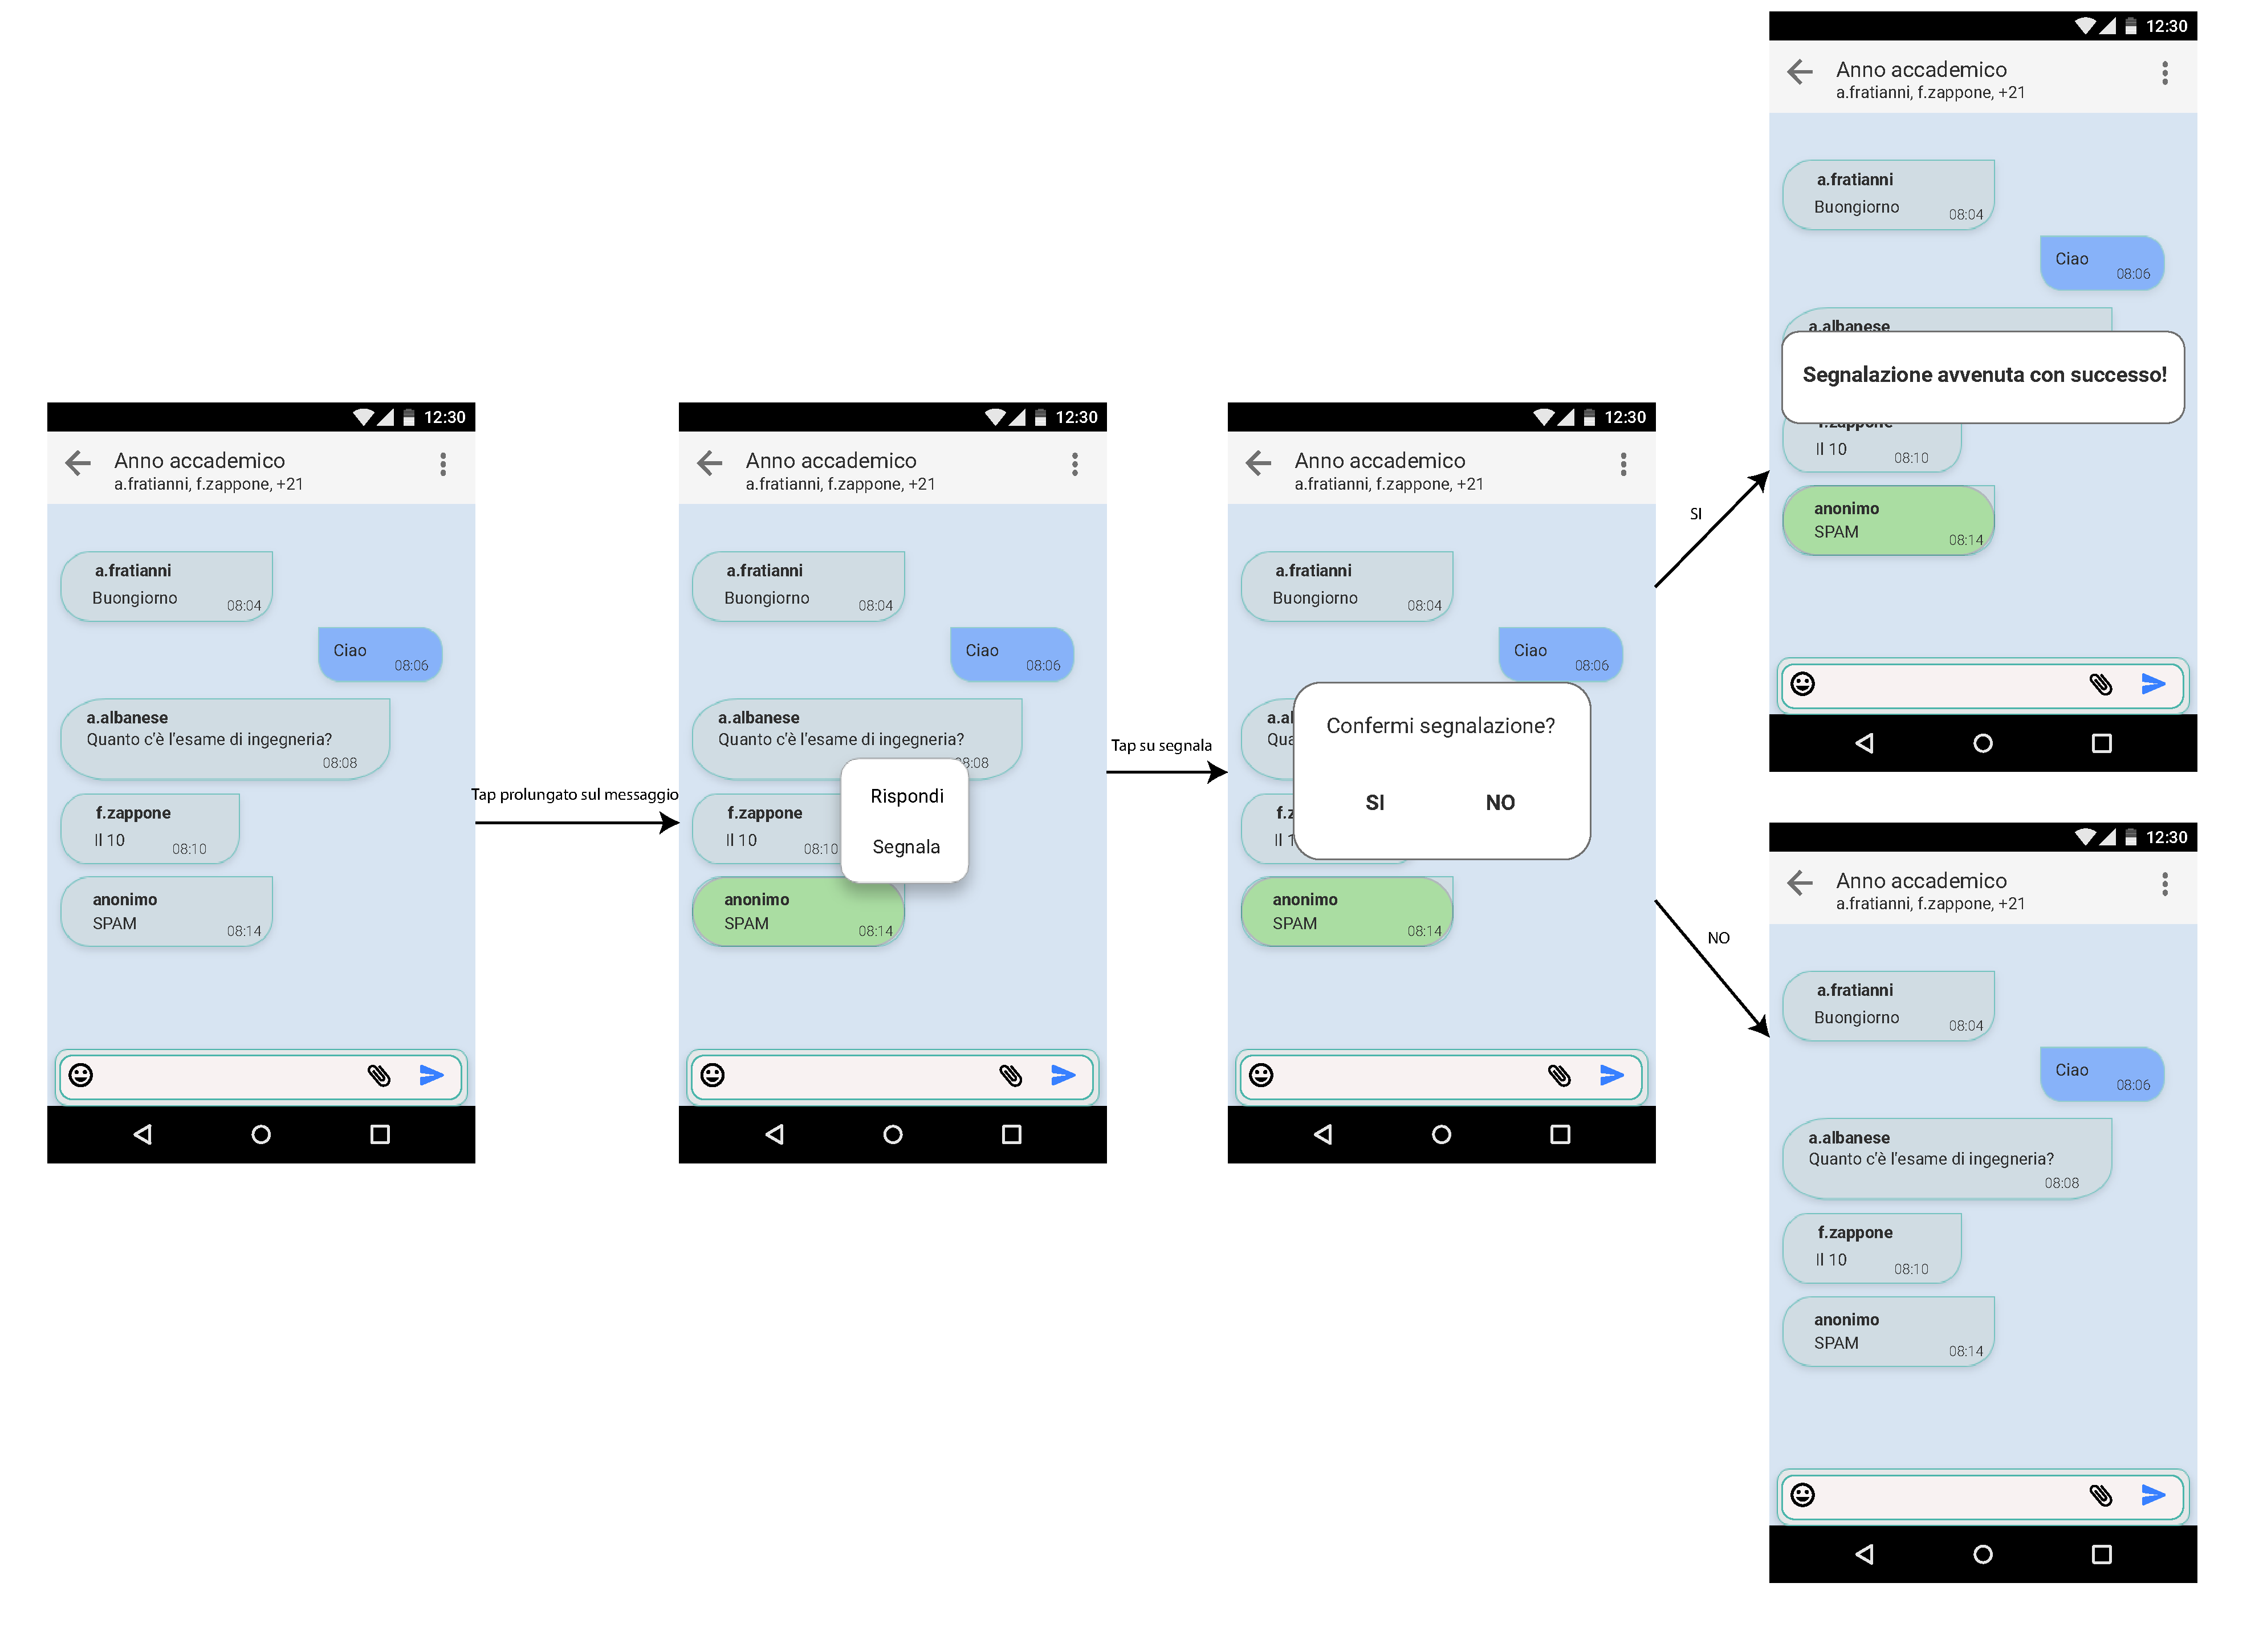
\includegraphics[width=0.9\textwidth]{imgs/gruppo6/activities/act_cus6_segnalazione_messaggio.pdf}
	\caption{CUS6 - Segnalazione messaggio}
	\label{fig:cus6}
\end{figure}

\begin{figure}
	\centering
	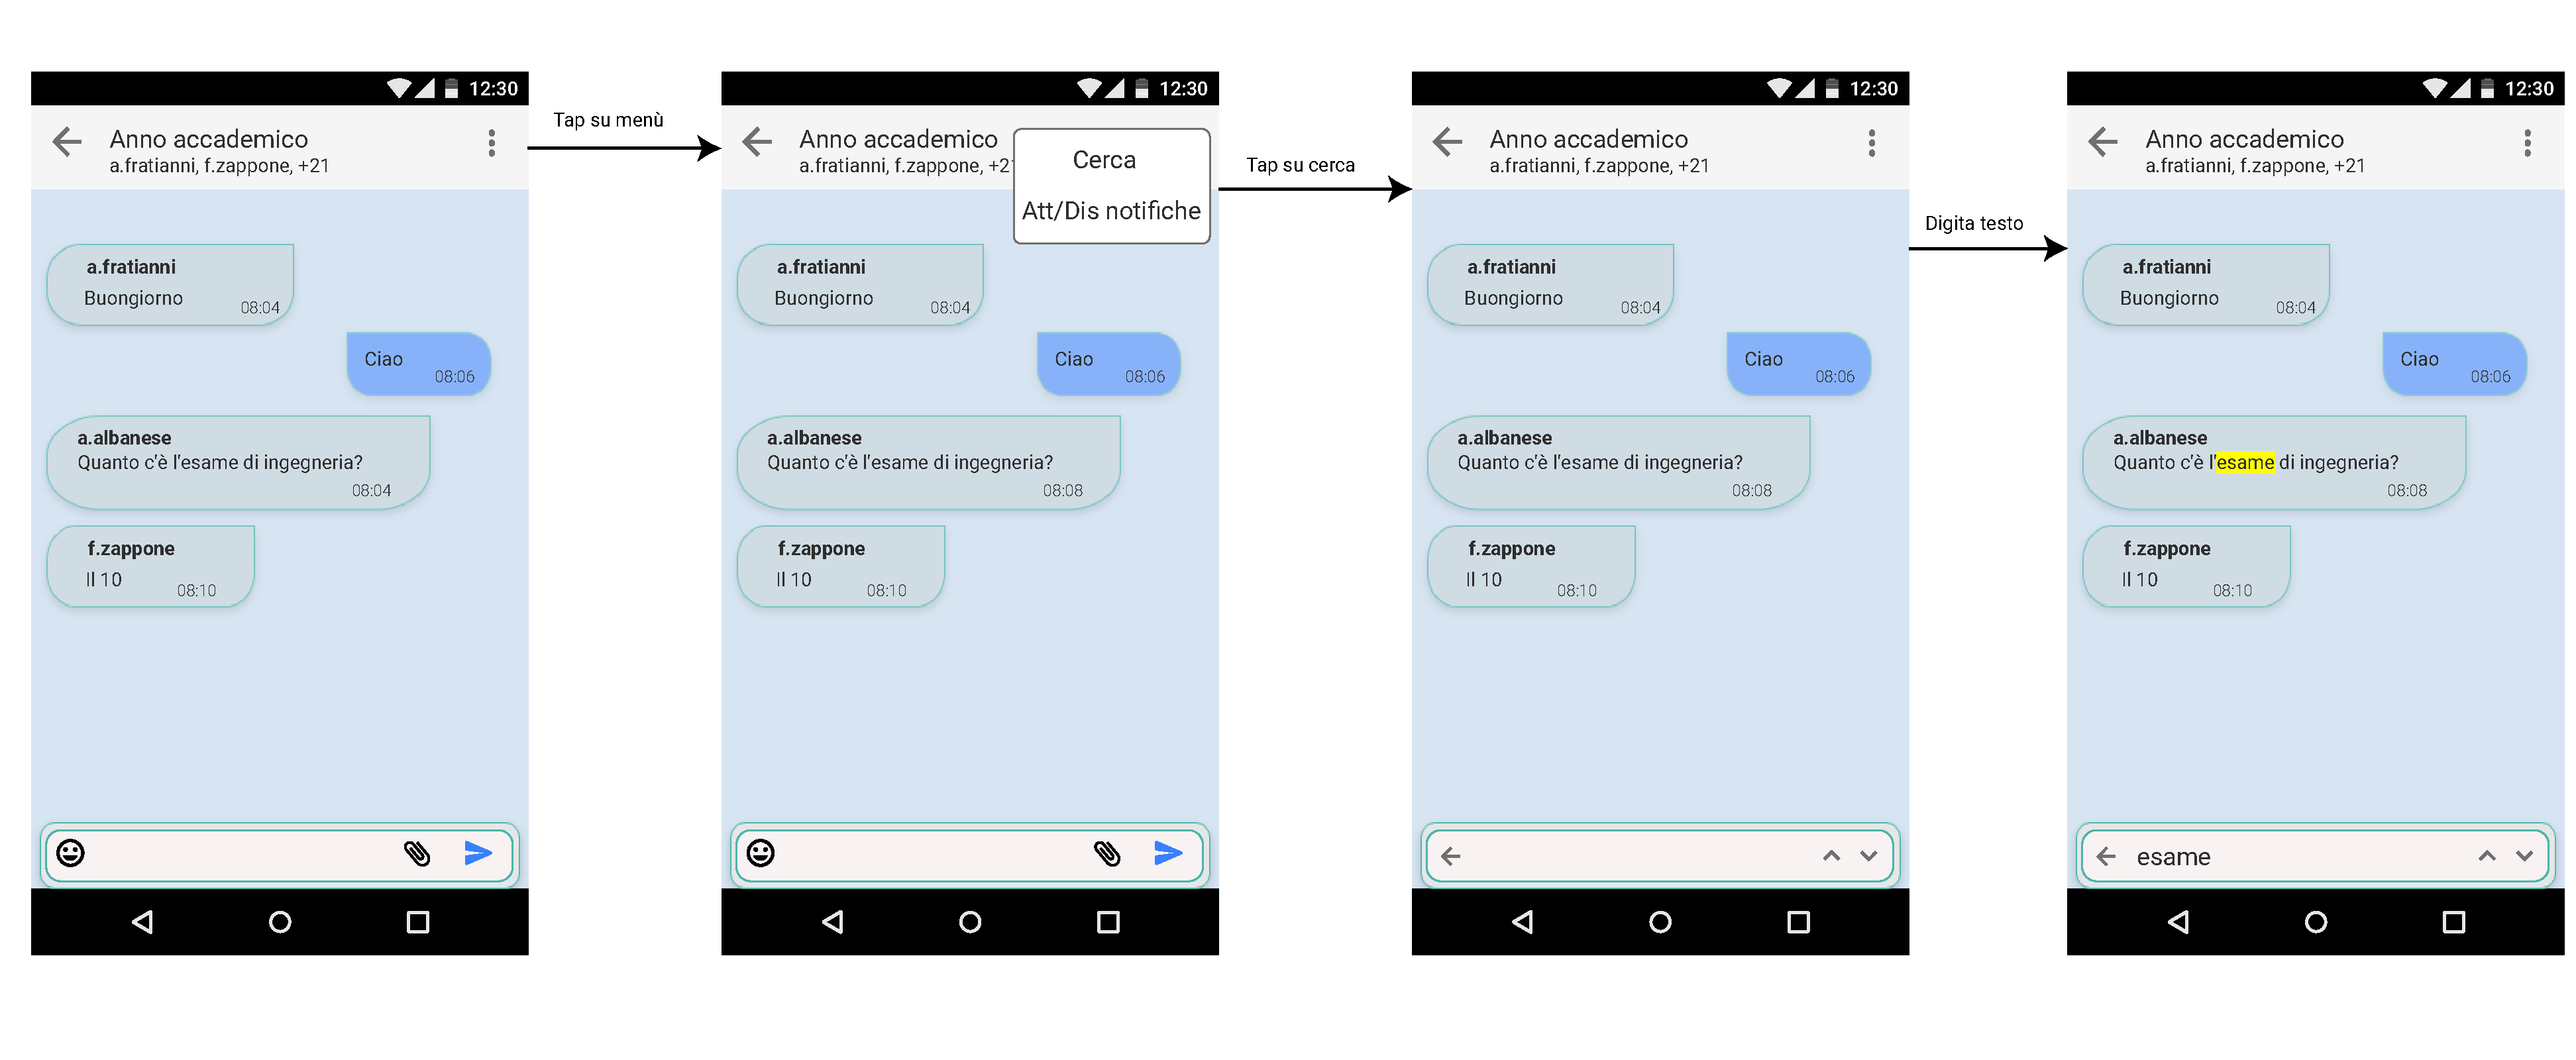
\includegraphics[width=0.9\textwidth]{imgs/gruppo6/activities/act_cus7_ricerca_testo_nella_chat.pdf}
	\caption{CUS7 - Ricerca testo nella chat}
	\label{fig:cus7}
\end{figure}

\begin{figure}
	\centering
	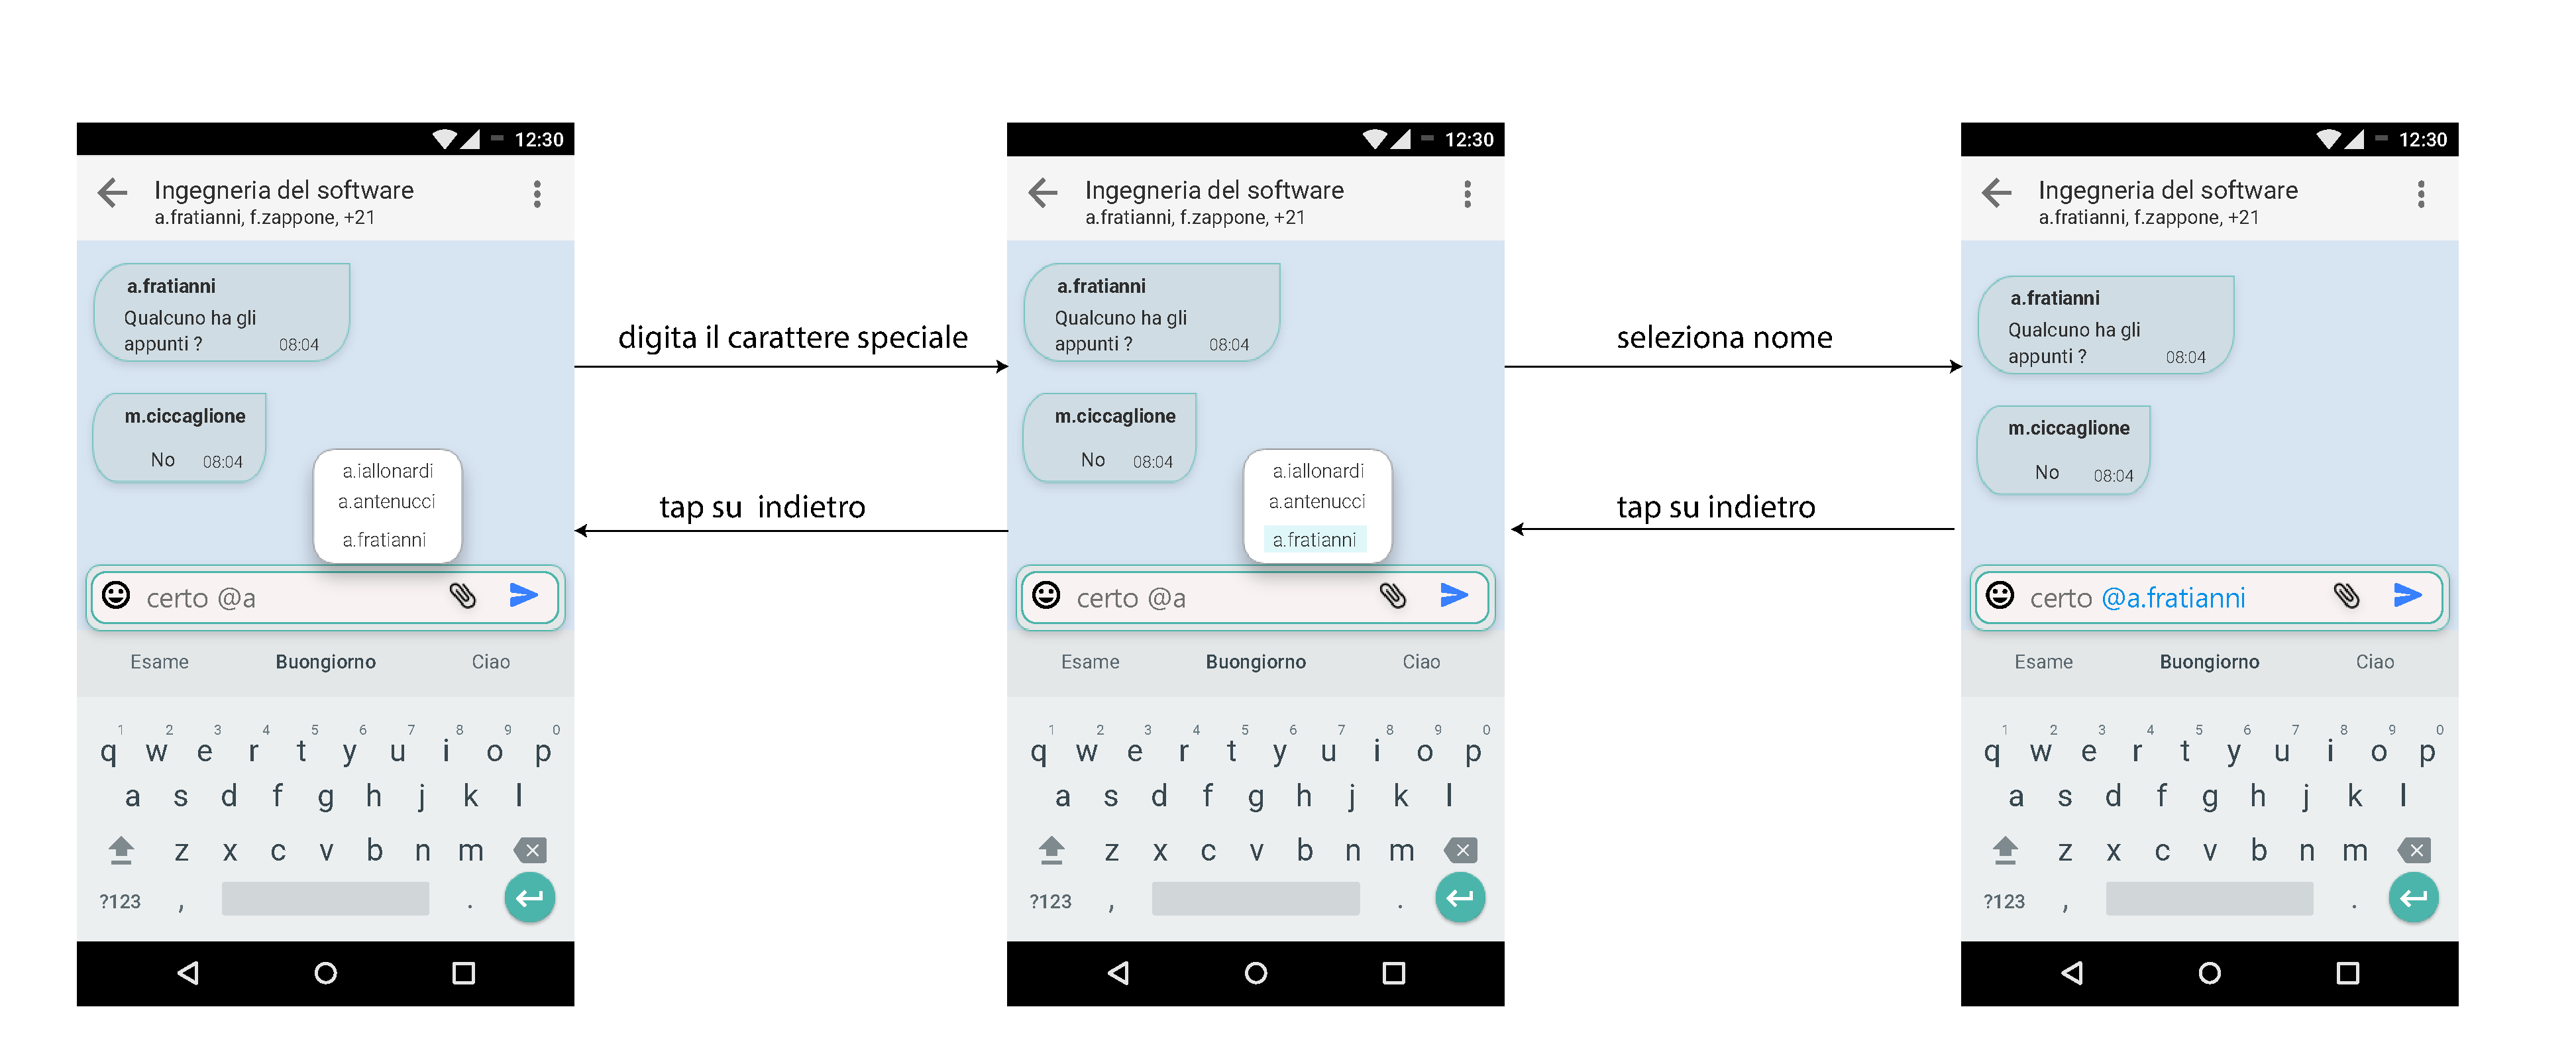
\includegraphics[width=0.9\textwidth]{imgs/gruppo6/activities/act_cus8_tag_membro_messaggio.pdf}
	\caption{CUS8 - Tag membro in messaggio}
	\label{fig:cus8}
\end{figure}

\begin{figure}
	\centering
	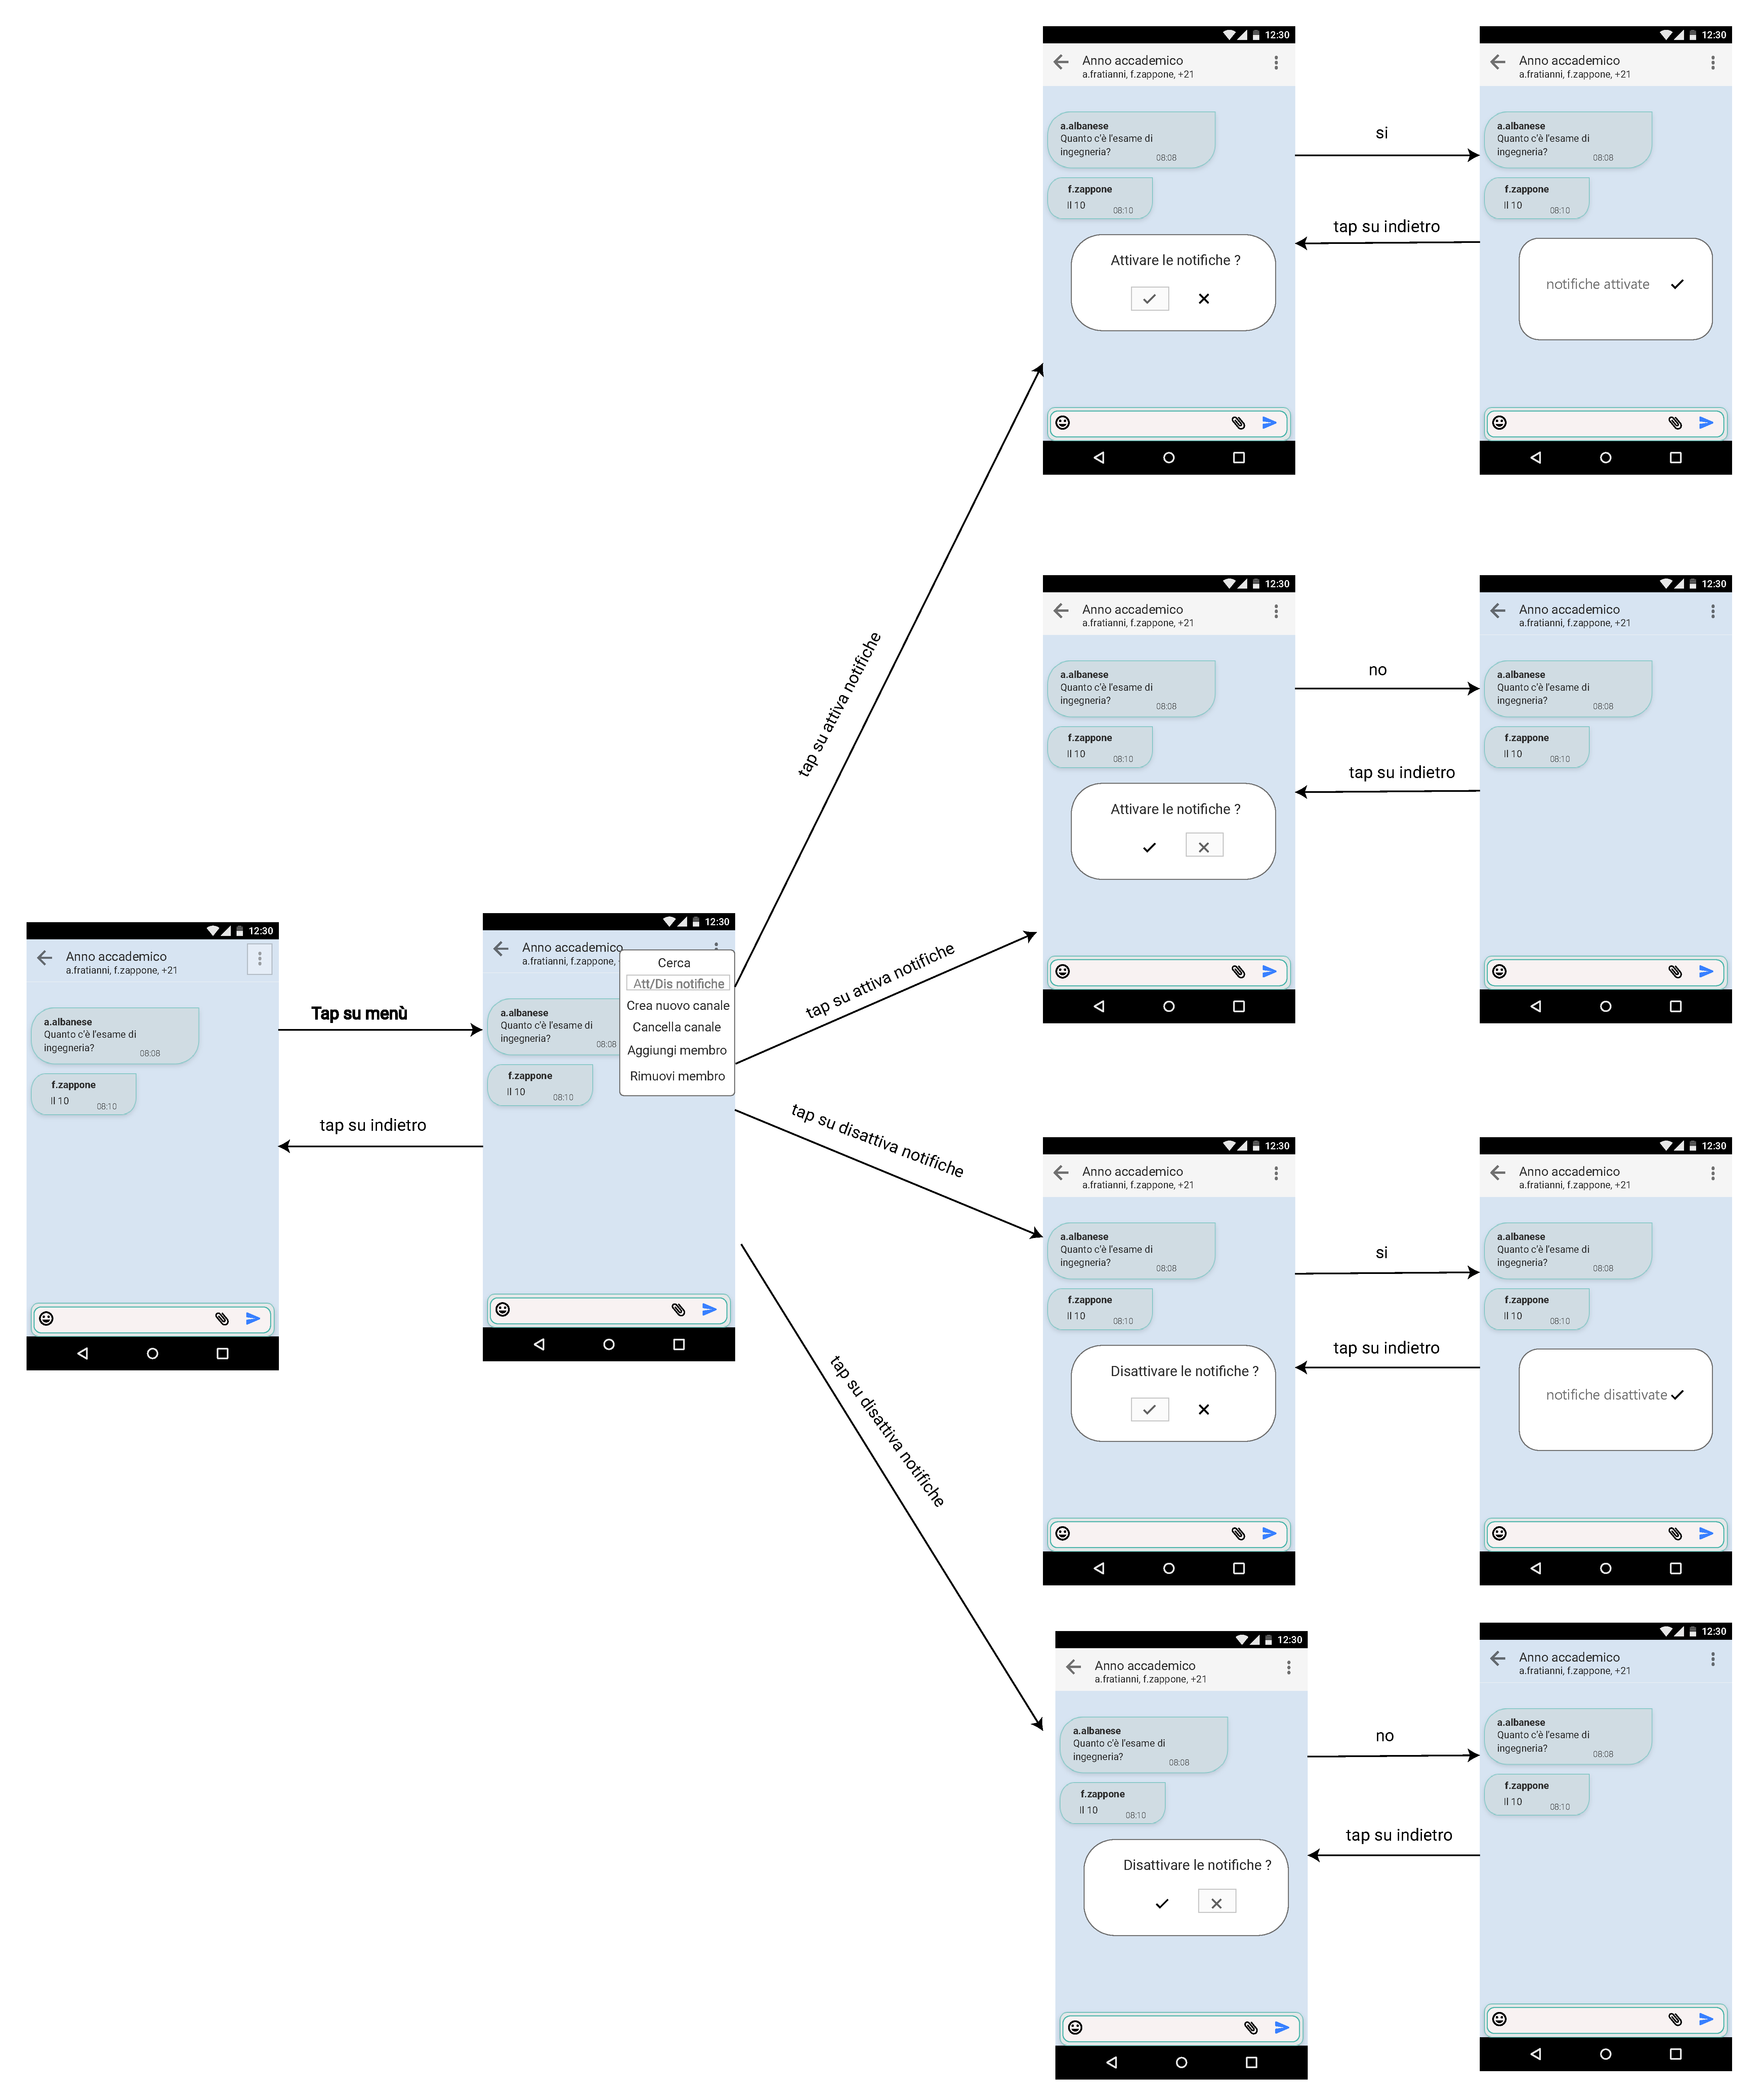
\includegraphics[width=0.9\textwidth]{imgs/gruppo6/activities/act_cus9_gestisci_notifiche_chat.pdf}
	\caption{CUS9 - Gestisci notifiche chat}
	\label{fig:cus9}
\end{figure}

\begin{figure}
	\centering
	\includegraphics[width=0.9\textwidth]{imgs/gruppo6/activities/act_cus10_seleziona_emoji.pdf}
	\caption{CUS10 - Selezione emoji}
	\label{fig:cus10}
\end{figure}

\begin{figure}
	\centering
	\includegraphics[width=0.9\textwidth]{imgs/gruppo6/activities/act_cus11_elenco_membri.pdf}
	\caption{CUS11 - Visualizza elenco membri chat}
	\label{fig:cus11}
\end{figure}
%%% END activities chat studenti %%%

%%% START activities chat docenti %%%
\pagebreak
\begin{figure}
\subsection{Activities relative alla chat dell'App Docenti}
	\centering
	\includegraphics[width=0.9\textwidth]{imgs/gruppo6/activities/act_cud1_creazione_canale.pdf}
	\caption{CUD1 - Creazione canale}
	\label{fig:cud1}
\end{figure}

\begin{figure}
	\centering
	\includegraphics[width=0.9\textwidth]{imgs/gruppo6/activities/act_cud2_cancella_canale.pdf}
	\caption{CUD2 - Cancellazione canale}
	\label{fig:cud2}
\end{figure}

\begin{figure}
	\centering
	\includegraphics[width=0.9\textwidth]{imgs/gruppo6/activities/act_cud3_aggiungi_membro_chat.pdf}
	\caption{CUD3 - Aggiungi membro ad un canale}
	\label{fig:cud3}
\end{figure}

\begin{figure}
	\centering
	\includegraphics[width=0.9\textwidth]{imgs/gruppo6/activities/act_cud4_rimuovi_membro_da_canale.pdf}
	\caption{CUD4 - Rimuovi membro da un canale}
	\label{fig:cud4}
\end{figure}

\begin{figure}
	\centering
	\includegraphics[width=0.9\textwidth]{imgs/gruppo6/activities/act_cud5_blocca_studente.pdf}
	\caption{CUD5 - Blocca Studente}
	\label{fig:cud5}
\end{figure}

\begin{figure}
	\centering
	\includegraphics[width=0.9\textwidth]{imgs/gruppo6/activities/act_cud5_blocca_studente2.pdf}
	\caption{CUD5 - Blocca Studente (es. 2}
	\label{fig:cud5-2}
\end{figure}

\begin{figure}
	\centering
	\includegraphics[width=0.9\textwidth]{imgs/gruppo6/activities/act_cud6_sblocca_da_elenco.pdf}
	\caption{CUD6 - Sblocca Studente (da elenco)}
	\label{fig:cud6}
\end{figure}

\begin{figure}
	\centering
	\includegraphics[width=0.9\textwidth]{imgs/gruppo6/activities/act_cud6_sblocca_da_messaggio.pdf}
	\caption{CUD6 - Sblocca Studente (da messaggio)}
	\label{fig:cud6}
\end{figure}
%%% END activities chat docenti %%%

%%% START activities chat pannello %%%
\pagebreak
\begin{figure}
\subsection{Activities relative al pannello di amministrazione}
	\centering
	\includegraphics[width=0.9\textwidth]{imgs/gruppo6/activities/act_cup1_login.pdf}
	\caption{CUP1 - Login}
	\label{fig:cup1}
\end{figure}

\begin{figure}
	\centering
	\includegraphics[width=0.9\textwidth]{imgs/gruppo6/activities/act_cup2_logout.pdf}
	\caption{CUP2 - Logout}
	\label{fig:cup2}
\end{figure}

\begin{figure}
	\centering
	\includegraphics[width=0.9\textwidth]{imgs/gruppo6/activities/act_cup3_filtro_chat_corsi1.pdf}
	\caption{CUP3 - Ricerca chat (filtri chat corsi - pt.1)}
	\label{fig:cup3}
\end{figure}

\begin{figure}
	\centering
	\includegraphics[width=0.9\textwidth]{imgs/gruppo6/activities/act_cup3_filtro_chat_corsi2.pdf}
	\caption{CUP3 - Ricerca chat (filtri chat corsi - pt.2)}
	\label{fig:cup3-2}
\end{figure}

\begin{figure}
	\centering
	\includegraphics[width=0.9\textwidth]{imgs/gruppo6/activities/act_cup3_filtro_chat_studenti1.pdf}
	\caption{CUP3 - Ricerca chat (filtri chat studenti - pt.1)}
	\label{fig:cup3-3}
\end{figure}

\begin{figure}
	\centering
	\includegraphics[width=0.9\textwidth]{imgs/gruppo6/activities/act_cup3_filtro_chat_studenti2.pdf}
	\caption{CUP3 - Ricerca chat (filtri chat studenti - pt.2)}
	\label{fig:cup3-4}
\end{figure}

\begin{figure}
	\centering
	\includegraphics[width=0.9\textwidth]{imgs/gruppo6/activities/act_cup3_ricerca_chat_corsi1.pdf}
	\caption{CUP3 - Ricerca chat (cerca corsi - pt.1)}
	\label{fig:cup3-5}
\end{figure}

\begin{figure}
	\centering
	\includegraphics[width=0.9\textwidth]{imgs/gruppo6/activities/act_cup3_ricerca_chat_corsi2.pdf}
	\caption{CUP3 - Ricerca chat (cerca corsi - pt.2)}
	\label{fig:cup3-6}
\end{figure}

\begin{figure}
	\centering
	\includegraphics[width=0.9\textwidth]{imgs/gruppo6/activities/act_cup3_ricerca_chat_studenti.pdf}
	\caption{CUP3 - Ricerca chat (cerca studenti - pt.1)}
	\label{fig:cup3-7}
\end{figure}

\begin{figure}
	\centering
	\includegraphics[width=0.9\textwidth]{imgs/gruppo6/activities/act_cup3_ricerca_chat_studenti2.pdf}
	\caption{CUP3 - Ricerca chat (cerca studenti - pt.2)}
	\label{fig:cup3-8}
\end{figure}

\begin{figure}
	\centering
	\includegraphics[width=0.9\textwidth]{imgs/gruppo6/activities/act_cup4_visualizza_lista_chat_corsi1.pdf}
	\caption{CUP4 - Visualizza lista chat (corsi - pt.1)}
	\label{fig:cup4}
\end{figure}

\begin{figure}
	\centering
	\includegraphics[width=0.9\textwidth]{imgs/gruppo6/activities/act_cup4_visualizza_lista_chat_corsi2.pdf}
	\caption{CUP4 - Visualizza lista chat (corsi - pt.2)}
	\label{fig:cup4-2}
\end{figure}

\begin{figure}
	\centering
	\includegraphics[width=0.9\textwidth]{imgs/gruppo6/activities/act_cup4_visualizza_lista_chat_studenti.pdf}
	\caption{CUP4 - Visualizza lista chat (studenti)}
	\label{fig:cup4-3}
\end{figure}

\begin{figure}
	\centering
	\includegraphics[width=0.9\textwidth]{imgs/gruppo6/activities/act_cup5_abilita_chat.pdf}
	\caption{CUP5 - Abilita chat}
	\label{fig:cup5}
\end{figure}

\begin{figure}
	\centering
	\includegraphics[width=0.9\textwidth]{imgs/gruppo6/activities/act_cup6_disabilita_chat.pdf}
	\caption{CUP6 - Disabilita chat}
	\label{fig:cup6}
\end{figure}

\begin{figure}
	\centering
	\includegraphics[width=0.9\textwidth]{imgs/gruppo6/activities/act_cup7_visualizza_canale.pdf}
	\caption{CUP7 - Visualizza canale}
	\label{fig:cup7}
\end{figure}

\begin{figure}
	\centering
	\includegraphics[width=0.9\textwidth]{imgs/gruppo6/activities/act_cup8_aggiungi_canale1.pdf}
	\caption{CUP8 - Aggiungi canale (pt.1)}
	\label{fig:cup8}
\end{figure}

\begin{figure}
	\centering
	\includegraphics[width=0.9\textwidth]{imgs/gruppo6/activities/act_cup8_aggiungi_canale2.pdf}
	\caption{CUP8 - Aggiungi canale (pt.2)}
	\label{fig:cup8-2}
\end{figure}

\begin{figure}
	\centering
	\includegraphics[width=0.9\textwidth]{imgs/gruppo6/activities/act_cup9_cancella_canale1.pdf}
	\caption{CUP9 - Cancella canale (pt.1)}
	\label{fig:cup9}
\end{figure}

\begin{figure}
	\centering
	\includegraphics[width=0.9\textwidth]{imgs/gruppo6/activities/act_cup9_cancella_canale2.pdf}
	\caption{CUP9 - Cancella canale (pt.2)}
	\label{fig:cup9-2}
\end{figure}

\begin{figure}
	\centering
	\includegraphics[width=0.9\textwidth]{imgs/gruppo6/activities/act_cup10_visualizza_lista_utenti.pdf}
	\caption{CUP10 - Visualizza lista utenti}
	\label{fig:cup10}
\end{figure}

\begin{figure}
	\centering
	\includegraphics[width=0.9\textwidth]{imgs/gruppo6/activities/act_cup11_aggiungi_utente_canale1.pdf}
	\caption{CUP11 - Aggiungi un utente ad un canale (pt.1)}
	\label{fig:cup11}
\end{figure}

\begin{figure}
	\centering
	\includegraphics[width=0.9\textwidth]{imgs/gruppo6/activities/act_cup11_aggiungi_utente_canale2.pdf}
	\caption{CUP11 - Aggiungi un utente ad un canale (pt.2)}
	\label{fig:cup11-2}
\end{figure}

\begin{figure}
	\centering
	\includegraphics[width=0.9\textwidth]{imgs/gruppo6/activities/act_cup12_cancella_utente_canale.pdf}
	\caption{CUP12 - Rimuovere un utente da un canale}
	\label{fig:cup12}
\end{figure}

\begin{figure}
	\centering
	\includegraphics[width=0.9\textwidth]{imgs/gruppo6/activities/act_cup13_silenziare_utente1.pdf}
	\caption{CUP13 - Silenziare utente in un canale (pt.1)}
	\label{fig:cup13}
\end{figure}

\begin{figure}
	\centering
	\includegraphics[width=0.9\textwidth]{imgs/gruppo6/activities/act_cup13_silenziare_utente2.pdf}
	\caption{CUP13 - Silenziare utente in un canale (pt.2)}
	\label{fig:cup13-2}
\end{figure}

\begin{figure}
	\centering
	\includegraphics[width=0.9\textwidth]{imgs/gruppo6/activities/act_cup14_reintegra_utente.pdf}
	\caption{CUP14 - Reintegra utente in un canale}
	\label{fig:cup14}
\end{figure}

\begin{figure}
	\centering
	\includegraphics[width=0.9\textwidth]{imgs/gruppo6/activities/act_cup15_modifica_permessi_utente1.pdf}
	\caption{CUP15 - Modificare i permessi di un utente in un canale (pt.1)}
	\label{fig:cup15-2}
\end{figure}

\begin{figure}
	\centering
	\includegraphics[width=0.9\textwidth]{imgs/gruppo6/activities/act_cup15_modifica_permessi_utente2.pdf}
	\caption{CUP15 - Modificare i permessi di un utente in un canale (pt.2)}
	\label{fig:cup15-2}
\end{figure}

\begin{figure}
	\centering
	\includegraphics[width=0.9\textwidth]{imgs/gruppo6/activities/act_cup16_nascondi_messaggio.pdf}
	\caption{CUP16 - Nascondi messaggio}
	\label{fig:cup16}
\end{figure}

\begin{figure}
	\centering
	\includegraphics[width=0.9\textwidth]{imgs/gruppo6/activities/act_cup17_reintegra_messaggio.pdf}
	\caption{CUP17  - Reintegra messaggio}
	\label{fig:cup17}
\end{figure}

\begin{figure}
	\centering
	\includegraphics[width=0.9\textwidth]{imgs/gruppo6/activities/act_cup18_invio_notifiche1.pdf}
	\caption{CUP18 - Invio Notifiche (pt.1)}
	\label{fig:cup18}
\end{figure}

\begin{figure}
	\centering
	\includegraphics[width=0.9\textwidth]{imgs/gruppo6/activities/act_cup18_invio_notifiche2.pdf}
	\caption{CUP18 - Invio Notifiche (pt.2)}
	\label{fig:cup18-2}
\end{figure}

\begin{figure}
	\centering
	\includegraphics[width=0.9\textwidth]{imgs/gruppo6/activities/act_cup19_gestione_messaggi_inopportuni.pdf}
	\caption{CUP19 - Gestione messaggi inopportuni}
	\label{fig:cup19}
\end{figure}
%%% END activities chat pannello %%%
\clearpage